\startexercise
\section{集合}
  \subsection{选择题}
  \begin{exercise}{\bf 选择题}
    \item 【集合,定义】\\
      设集合$A=\{x\in\mathbb{Q}\mid x>1\}$,则\xz
        \xx{$\varnothing\in A$}
        {$\sqrt2\notin A$}
        {$\sqrt2\in A$}
        {$\{\sqrt2\}\subseteq A$}
      \begin{answer}
        B
      \end{answer}
    \item 【集合,补集、计算】【福州三中高一半期考】\\
      (福州三中高一半期考)已知全集$U=\{-2,-1,2,3,4\}$,集合$A=\{-1,2,3\}$,$B=\{-2,2\}$,则$(\complement_UA)\bigcup B=$\xz
      \xx{$\{-2\}$}
        {$\{-2,2,4\}$}
        {$\{-2,-1,2\}$}
        {$\{-2,2,3,4\}$}
      \begin{answer}
        B
      \end{answer}
    \item 【集合,新定义】\\
      对于集合$M,N$,定义$M-N=\{x\mid x\in M,\text{且}x\notin N\}$,$M\oplus N=(M-N)\cup(N-M)$,设$A=\Bigl\{x\Bigm| x\geq-\dfrac{9}4\Bigr\}$,$B=\{x\mid x<0\}$,则$A\oplus B=$\xz
        \xx{$(-\dfrac{9}4,0]$}
        {$[-\dfrac{9}4,0)$}
        {$(-\infty,-\dfrac{9}4)\bigcup[0,+\infty)$}
        {$(-\infty,-\dfrac{9}4]\bigcup(0,+\infty)$}
      \begin{answer}
        C
      \end{answer}
    \item 福州三中高一上数学期中卷(2017-2018).doc【集合,补集、子集、参数】\\
      (17-18三中高一上期中考17)(本小题满分10分)已知全集 $U=\mathbb{R}$,集合$A=\{x\mid (x-3)(x+2)\leq0\} $,$B=\{x\mid 2a\leq x\leq a+2,a\in \mathbb{R} \} $.\\
      (I)若$a=-2 $,求集合$(\complement_UA)\bigcup B $;
      (II)若$B\subseteq A $,求实数$a $的取值范围.
      \begin{answer}
       (I) $\{x\mid-4\leq x<-2 \} $
       (II) $[-1,1]\cup[2,+\infty] $
      \end{answer}
    \item 《2019金考卷双测20套(文)ISBN978-7-5371-9890-5》题型1集合的运算P1p1【2018•全国I卷】【集合,交集】\\
      \source{2018文}{全国I卷}
      已知集合$A=\{0,2\}$,$B=\{-2,-1,0,1,2\}$,则$A\cap B=$\xz
      \xx{$\{0,2\}$}
       {$\{1,2\}$}
       {$\{0\}$}
       {$\{-1,-2.0,1,2\}$}
      \begin{answer}
        $\{1,8\}$
      \end{answer}
    \item 《2019金考卷双测20套(文)ISBN978-7-5371-9890-5》题型1集合的运算P1p2【2018•天津卷】【集合,补集交集,区间】\\
      \source{2018文}{天津卷}
      设全集为$\mathbb{R}$,集合$A=\{x\mid 0<x<2\}$,$B=\{x\mid x\geqslant1\}$,
      则$A\bigcap\bigl(\complement_{\mathbb R}B\bigr)=$\xz
      \xx{$\{x\mid 0<x\leqslant1\}$}
       {$\{x\mid 0<x<1\}$}
       {$\{x\mid 1\leqslantx<2\}$}
       {$\{x\mid 0<x<2\}$}
      \begin{answer}
        B
      \end{answer}
    \item 《2019金考卷双测20套(文)ISBN978-7-5371-9890-5》题型1集合的运算P1p3【2018•全国II卷】【集合,元素】\\
      \source{2018文}{全国II卷}
      已知集合$A=\{(x,y)\mid x^2+y^2\leqslant3,x\inZ,y\inZ\}$,则$A$中元素的个数为\xz
      \xx{9}{8}{5}{4}
      \begin{answer}
        A
      \end{answer}
    \item 《2019金考卷双测20套(文)ISBN978-7-5371-9890-5》题型1集合的运算P1p4【2018•济南模拟】【集合,并集,二次方程】\\
      \source{2018文}{济南模拟}
      已知集合$A=\{x\mid x^2+2x-3=0\}$,$B=\{-1,1\}$则$A\cup B=$\xz
      \xx{$\{1\}$}
       {$\{-1,1,3\}$}
       {$\{-3,-1,1\}$}
       {$\{-3,-1,1,3\}$}
      \begin{answer}
        C
      \end{answer}
        \item 《2019金考卷双测20套(文)ISBN978-7-5371-9890-5》题型1集合的运算P1p5【2018•贵阳期末】【集合,交集,根式定义域】\\
          \source{2018文}{贵阳期末}
          设$A=\{x\mid -1<x<2\}$,$B=\{x\mid y=\sqrt{-x+1}\}$,则$A\cap B=$\xz
          \xx{$(-1,1]$}
           {$(-5,2)$}
           {$(-3,2)$}
           {$(-3,3)$}
          \begin{answer}
            A
          \end{answer}
    \item 《2019金考卷双测20套(文)ISBN978-7-5371-9890-5》题型1集合的运算P1p7【2018•郑州二测】【集合,并集,对数】\\
      \source{2018文}{郑州二测}
      已知集合$A=\{x\inR\mid \log_2(3-x)\leqslant 1\}$,$B=\{x\inR\mid 0\leqslant x\leqslant 2\}$,则$A\cup B=$\xz
      \xx{$[0,3]$}
       {$[1,2]$}
       {$[0,3)$}
       {$[1,3]$}
      \begin{answer}
        C
      \end{answer}
    \item 《2019金考卷双测20套(文)ISBN978-7-5371-9890-5》题型1集合的运算P1p8【2018•南昌调研】【集合,交集,对数】\\
      \source{2018文}{南昌调研}
      设集合$A=\{x\mid -2\leqslant x\leqslant 1\}$,$B=\{x\mid y=\log_2{(x^2-2x-3)}\}$,则$A\cap B=$\xz
      \xx{$[-2,1)$}
       {$(-1,1]$}
       {$[-2,-1)$}
       {$[-1,1)$}
      \begin{answer}
        C
      \end{answer}
    \item 《2019金考卷双测20套(文)ISBN978-7-5371-9890-5》题型1集合的运算P1p9【2018•合肥一检】【集合,交集,定义域,值域】\\
      \source{2018文}{合肥一检}
      已知集合$M$是函数$y=\dfrac1{\sqrt{1-2x}}$的定义域,集合$N$是函数$y=x^2-4$的值域,则$M\cap N=$\xz
      \xx{$\{x\mid x\leqslant \dfrac12\}$}
       {$\{x\mid -4\leqslant x< \dfrac12\}$}
       {$\{(x,y)\mid x< \dfrac12\text{且}\geqslant -4\}$}
       {$\varnothing$}
      \begin{answer}
        B
      \end{answer}
    \item 《2019金考卷双测20套(文)ISBN978-7-5371-9890-5》题型1集合的运算P1p10【2018•福州质检】【集合,元素,交集】\\
      \source{2018文}{福州质检}
      已知集合$A=\{x\mid x=2k+1,k\inZ\}$,$B=\{x\mid -1<x\leqslant4\}$,则集合$A\cap B$中元素的个数为\xz
      \xx{1}{2}{3}{4}
      \begin{answer}
        B
      \end{answer}
    \item 《2019金考卷双测20套(文)ISBN978-7-5371-9890-5》题型1集合的运算P1p11【2018•惠州二调】【集合,交集,二次不等式】\\
      \source{2018文}{惠州二调}
      已知集合$A=\{x\mid x<a\}$,$B=\{x\mid x^2-3x+2<0\}$,若$A\cap B=B$,则实数$A$的取值范围是\xz
      \xx{$(-\infty,1)$}
       {$(-\infty,1]$}
       {$(2,+\infty)$}
       {$[2,+\infty)$}
      \begin{answer}
        D
      \end{answer}
    \item 《2019金考卷双测20套(文)ISBN978-7-5371-9890-5》题型1集合的运算P1p15【2018•广州一测】【集合运算,分式不等式】\\
      \source{2018文}{广州一测}
      设集合$A=\Bigl\{x\Bigm| \dfrac{x+3}{x-1}<0\Bigr\}$,$B=\{x\mid x\leqslant{-3}\}$,则集合$\{x\mid x\geqslant1\}=$\xz
      \xx{$A\cap B$}
       {$A\cup B$}
       {$\bigl(\complement_{\RR}A\bigr)\cup \bigl(\complement_{\RR}B\bigr)$}
       {$\bigl(\complement_{\RR}A\bigr)\cap \bigl(\complement_{\RR}B\bigr)$}
      \begin{answer}
        D
      \end{answer}
  \end{exercise}
  \subsection{填空题}
  \begin{exercise}{\bf 填空题}
    \item 【集合,交集、计算】【福州三中高一半期考】\\
      (福州三中高一半期考)设集合$M=\{x\in \mathbb{R}\mid x-1<0 \} $, $N=\{y\mid y=x^2,x\in\mathbb{R} \} $,则$M\cap N$\tk
      \begin{answer}
        $[0,1)$
      \end{answer}
    \item 《2019金考卷双测20套(文)ISBN978-7-5371-9890-5》题型1集合的运算P1p16【2018•江苏卷】【集合,交集】\\
      \source{2018文}{江苏卷}
      已知集合$A=\{0,1,2,8\}$,$B=\{-1,1,6,8\}$,那么$A\cap B=$\tk.
      \begin{answer}
        $\{1,8\}$
      \end{answer}
    \item 《2019金考卷双测20套(文)ISBN978-7-5371-9890-5》题型1集合的运算P1p17【2018•陕西摸底检测】【集合,交集、补集,二次不等式】\\
      \source{2018文}{陕西摸底检测}
      已知集合$U=\mathbb{Z}$,集合$A=\{x\inZ\mid 3\leqslant x<7\}$,$B=\{x\inZ\mid x^2-7x+10>0\}$,则$A\bigcap\bigl(\complement_UB\bigr)=$\tk.
      \begin{answer}
        $\{3,4,5\}$
      \end{answer}
  \end{exercise}
  \subsection{解答题}
  \begin{exercise}{\bf 解答题}
    \item 福州三中高一上数学七中卷(2017-2018).doc【集合,参数】【17-18三中高一上期中考17】\\
      (17-18三中高一上期中考17)(本小题满分12分)已知全集 $U=\mathbb{R}$,集合$A=\{x\mid (x-3)(x+2)\leq0\} $,$B=\{x\mid 2a\leq x\leq a+2,a\in \mathbb{R} \} $.\\
      (I)若$a=-2 $,求集合$(\complement_UA)\bigcup B $;
      (II)若$B\subseteq A $,求实数$a $的取值范围.
      \begin{answer}
       (I) $\{x\mid -4\leq x<-2 \} $
       (II) $[-1,1]\cup[2,+\infty] $
      \end{answer}
    \item 【集合,交集、参数】\\
      (本小题满分10分)\\
      设集合$A=\{x\mid 2\leq x\leq4\}$,$B=\{x\mid 0<\ln x<1\}$,$C=\{x\mid t+1<x<2t,t\in\mathbb{R}\}$.\\
      (I)求$A\cap B$\\
      (II)求$A\cap C=C$,求$t$的取值范围.\\
      \begin{answer}
      解:(I)$\because$ $B=\{x\mid 1<x<\mathrm{e}\}$,$\therefore$$A\cup B=\{x\mid 2\leq x<\mathrm{e}\}$\\
      (II)$\because$ $A\cup C=C$,$\therefore$ $C\subseteq A$\\
      $C=\varnothing$时,$t+1\geq 2t$,$t\leq 1$\\
      $C\neq\varnothing$时,
      $\begin{cases}
        t+1<2t\\
        t+1\geq 2\\
        2t\leq 4
      \end{cases}
      $
      $\therefore$ $1<t\leq 2$\\
      综上,$t\in (-\infty,2]$
      \end{answer}
    \item 【集合,补集、并集、参数】【格致中学高一半期考】\\
      (格致中学高一半期考)已知集合$M=\{-2\leq x\leq 5\} $,$N=\{x\mid a+1\leq x\leq 2a+1\} $.
      (1)若$a=3 $,求$M\displaystyle \bigcap(\complement_{\mathbb{R} }{\large N}) $;
      (2)若$M\cup N=M $,求实数$a $的取值范围.
      \begin{answer}
        (1) $[-2,4)$
        (2) $(-\infty,2] $
      \end{answer}
  \end{exercise}
\section{函数}
  \subsection{课前检测}\begin{exercise}{\heiti 课前检测}\\
    \item
      填写下表,写出各函数的定义域、值域 、单调性以及奇偶性.
      \begin{center}
        \renewcommand{\arraystretch}{1.4}
        \begin{tabular}{|c|c|c|c|c|}
          \hline
        $f(x)$&\mbox{\hspace{1.5em}定义域\hspace{1.5em}}&\mbox{\hspace{2em}值域\hspace{2em}}&\mbox{\hspace{8em}单调性\hspace{8em}}&\mbox{\hspace{1.2em}奇偶性\hspace{1.2em}}\\
          \hline
          $x$&&&&\\
          \hline
          $x^2$&&&&\\
          \hline
          $\log_2x$&&&&\\
          \hline
          $3^x$&&&&\\
          \hline
          $\dfrac{1}{x}$&&&&\\
          \hline
          $\sqrt{x}$&&&&\\
          \hline
          $\log_x2$&&&&\\
          \hline
        \end{tabular}\\
      \end{center}
    \item 函数$y=\sqrt{32-2^x}$的定义域是\tk.
      \begin{answer}
       $(-\infty,5]$(或写为$\{x\mid x\leqslant5\}$)

     \item %【对数,指数,幂运算】\\
       若集合$A=\{y\mid y=2^x,x\inR\}$,$B=\{x\mid y=2^x,x\inR\}$则下列结论错误的是\xz
       \xx{$A\cap B=A$}
        {$A\cap B=\varnothing$}
        {$A\cup B=\RR$}
        {$A\cup B=B$}
        \begin{answer}
          B
        \end{answer}
      \item %【对数,指数,幂运算】\\
        若集合$A=\{y\mid y=2^x,x\inR\}$,$B=\{x\mid y=2^x,x\inR\}$则下列结论错误的是\xz
        \xx{$A\cap B=A$}
         {$A\cap B=\varnothing$}
         {$A\cup B=\RR$}
         {$A\cup B=B$}
         \begin{answer}
           B
         \end{answer}\end{answer}
    \item %【集合,指数,函数定义域】\\
      若集合$A=\{y\mid y=2^x,x\inR\}$,$B=\{x\mid y=2^x,x\inR\}$则下列结论错误的是\xz
      \xx{$A\cap B=A$}
       {$A\cap B=\varnothing$}
       {$A\cup B=\RR$}
       {$A\cup B=B$}
      \begin{answer}
        B
      \end{answer}
    \end{exercise}
  \subsection{选择题}\begin{exercise}{\bf 选择题}
    \item 【函数,求值】【福州高级中学16-17高一期中考】\\
      (福州高级中学16-17高一期中考)已知函数$f(x+1)=2x+5$,则$f(3)=$\xz
      \xx{5}{7}{9}{11}
      \begin{answer}
        C
      \end{answer}
    \item 【函数,定义域】\\
      函数$f(x)=\sqrt{2^x-1}$的定义域是\xz
      \xx{$ \left[0,+\infty\right)$}
       {$ \left[1,+\infty\right)$}
       {$ \left(-\infty,0\right]$}
       {$ \left(-\infty,1\right]$}
      \begin{answer}
        A
      \end{answer}
    \item 【函数,定义域】\\
      设函数$f(x)=\lg \dfrac{2+x}{2-x}$,则$ f\left(\dfrac{x}{2}\right)+f\left(\dfrac{2}{x}\right) $的定义域为\xz
      \xx{$\left(-4,0\right)\bigcup \left(0,4\right) $}
       {$\left(-4,-1\right)\bigcup \left(1,4\right) $}
       {$ \left(-2,-1\right)\bigcup \left(1,2\right)$}
       {$ \left(-4,-2\right)\bigcup \left(2,4\right)$}
      \begin{answer}
        B
      \end{answer}
    \item 【函数,定义域】\\
      函数$f(x)=\dfrac{1}{\sqrt{\left(\log_2x\right)^2-1}}$的定义域为\xz
      \xx{$ \left(0,\dfrac{1}{2}\right)$}
       {$ \left(2,+\infty\right)$}
       {$ \left(0,\dfrac{1}{2}\right)\bigcup\left(2,+\infty\right)$}
       {$ \left(0,\dfrac{1}{2}\right]\bigcup\left[2,+\infty\right)$}
      \begin{answer}
        C
      \end{answer}
    \item 【函数,定义域、抽象、复合】\\
      已知函数$f(x)$的定义域为$(-1,0)$,则函数$f(2x+1)$的定义域为\xz
      \xx{$(-1,1)$}{$\left(-1,-\dfrac{1}{2}\right)$}{$(-1,0)$}{$\left(\dfrac{1}{2},1\right)$}
      \begin{answer}
        B
      \end{answer}
    \item 【函数,定义域、抽象、复合】\\
      已知函数$f(2x+1)$的定义域为$\left(-2,\dfrac{1}{2}\right)$,则函数$f(x)$的定义域为\xz
      \xx{$ \left(-\dfrac{3}{2},-\dfrac{1}{4}\right)$}{$ \left(-1,\dfrac{3}{2}\right)$}{$ \left(-3,2\right)$}{$ \left(-3,3\right)$}
      \begin{answer}
        C
      \end{answer}
    \item 【函数,三要素】\\
      下列函数中,其定义域和值域分别与函数$y=10^{\lg x}$的定义域和值域相同的是\xz
      \xx{$y=x$}{$y=\lg x$}{$y=2^x$}{$y=\dfrac{1}{\sqrt{x}}$}
      \begin{answer}
        D
      \end{answer}
    \item 【函数,图像】\\
      下列函数中与函数$y=x(x\geq 0)$有相同图像的一个是\xz
        \xx{$ y=\dfrac{x^2}x $}
        {$y=\sqrt{x^2}$}
        {$y=\sqrt[3]{x^3}$}
        {$y=( \sqrt x)^2 $}
      \begin{answer}
        D
      \end{answer}
    \item 【函数,单调性】\\
      下列函数在区间$(0,+\infty) $上是增函数的是\xz
        \xx{$y=\ln(x+1)$}
         {$y=(x-1)^2$}
         {$y=x^{-2}$}
         {$y=3^{-x}$}
      \begin{answer}
        A
      \end{answer}
    \item 【函数,单调性】\\
      设$f(x),\ g(x)$都是单调函数,有如下四个命题:\\
      \ding{192}若$f(x)$单调递增,$g(x)$单调递增,则$f(x)-g(x)$单调递增;\\
      \ding{193}若$f(x)$单调递增,$g(x)$单调递减,则$f(x)-g(x)$单调递增;\\
      \ding{194}若$f(x)$单调递减,$g(x)$单调递增,则$f(x)-g(x)$单调递减;\\
      \ding{195}若$f(x)$单调递减,$g(x)$单调递减,则$f(x)-g(x)$单调递减;\\
      其中,正确的命题是\xz
      \xx{\ding{192}\ding{194}}{\ding{192}\ding{195}}{\ding{193}\ding{194}}{\ding{193}\ding{195}}
      \begin{answer}
        C
      \end{answer}
    \item 【函数,单调性】\\
      函数$y=-\sqrt{1-4x^2}$的单调递减区间是\xz
      \xx{$\left(-\infty,\dfrac{1}2\right]$}
        {$\left[\dfrac{1}2,+\infty\right)$}
        {$\left[-\dfrac{1}2,0\right]$}
        {$\left[0,\dfrac{1}2\right]$}
      \begin{answer}
        C
      \end{answer}
    \item 【函数,单调性、不等式】\\
      设奇函数$f(x)$在$ \left(0,+\infty\right) $上增函数且$ f(1)=0 $,则不等式$ \dfrac{f(x)-f(-x)}{x}<0 $的解集为\xz
      \xx{$ \left(-1,0\right)\bigcup \left(1,+\infty\right)$}{$ \left(-\infty,-1\right)\bigcup \left(0,1\right)$}{$ \left(-\infty,-1\right)\bigcup \left(1,+\infty\right)$}{$ \left(-1,0\right)\bigcup \left(0,1\right)$}
      \begin{answer}
        D
      \end{answer}
    \item 【函数,奇偶性】\\
      设函数$f(x),g(x)$的定义域都为$\mathbf{R}$,且$f(x)$是奇函数,$g(x)$是偶函数,则下列结论正确的是\xz
      \xx{$f(x)g(x)$是偶函数}{$\abs{f(x)}g(x)$是奇函数}{$f(x)\abs{g(x)}$是奇函数}{$\abs{f(x)g(x)}$是奇函数}
      \begin{answer}
        C
      \end{answer}
    \item 【函数,奇偶性】\\
      如果$f(x)$是定义在$\mathbf{R}$上的奇函数,那么下列函数中一定是偶函数的是\xz
      \xx{$ x+f(x)$}
       {$ xf(x)$}
       {$ x^2+f(x)$}
       {$ x^2f(x)$}
      \begin{answer}
        B
      \end{answer}
    \item 【函数,奇偶性、求值】\\
      已知函数$f(x)=\ln \left(\sqrt{1+9x^2}-3x\right)+1$,则$ f(\lg2)+f\left(\lg\dfrac{1}{2}\right) $等于\xz
      \xx{$-1$}{$0$}{$1$}{$2$}
      \begin{answer}
        D
      \end{answer}
    \item 【函数,奇偶性、求值】\\
      奇函数$f(x)$的定义域为$ \mathbf{R} ,~$若$ f(x+2) $为偶函数,且$ f(1)=1,~ $则 $f(8)+f(9)=$\xz
      \xx{$ -2 $}{$ -1 $}{$ 0 $}{$ 1 $}
      \begin{answer}
        D
      \end{answer}
    \item 【函数,奇偶性,求值】\\
      已知函数$g(x)=f(x)-x$是偶函数,且$ f(3)=4 $,则$ f(-3)= $\xz
      \xx{$-4$}{$-2$}{$0$}{$4$}
      \begin{answer}
        B
      \end{answer}
    \item 【函数,奇偶性、单调性、参数】\\
      已知函数$f(x)$是定义在$ \mathbf{R} $上的偶函数,且在区间$ \left[0,+\infty\right) $上单调递增,若实数$ a $满足$ f(\log_2a) +f(\log_\frac{1}{2}a)\le 2f(1)$,则$ a $的取值范围是\xz
      \xx{$ \left[1,2\right]$}{$ \left(0,\dfrac{1}{2}\right]$}{$ \left[\dfrac{1}{2},2\right]$}{$ \left(0,2\right]$}
      \begin{answer}
        C
      \end{answer}
    \item 【函数,单调性、奇偶性】【福建师大附中15-16高一期中考,6】\\
      (福建师大附中15-16高一期中考,6)下列函数中,既是偶函数又在$(0,+\infty)$单调递增的函数是\xz
      \xx{$y=x^3$}{$y=|x|+1$}{$y=-x^2+1$}{$y=2^{-|x|}$}
    \item 【函数,单调性、奇偶性、大小】【福州八中 15-16 高一期中考,2】\\
      (福州八中 15-16 高一期中考,2)设偶函数 $f(x)$的定义域为$\mathbb{R}$,当 $x\in[0,+\infty)$时,$f(x)$是增函数,则$f(-2)$,$f(\pi)$,$f(-3)$的大小关系是\xz
      \xx{$f(\pi)>f(-3)>f(-2)$}
          {$f(\pi)>f(-2)>f(-3)$}
          {$f(\pi)<f(-3)<f(-2)$}
          {$f(\pi)<f(-2)<f(-3)$}
    \item 【函数,单调性、奇偶性】【福州高级中学 16-17 高一期中考,11】\\
      (福州高级中学 16-17 高一期中考,11)定义在 $\mathbb{R}$上的偶函数$f(x)$,当$x\in[1,2]$时,$f(x)<0$且$f(x)$增函数,给出下列四个结论:\\
      (1)$f(x)$在$[-2,-1]$上单调递增;\hspace{4em}(2)当$x\in[-2,-1]$时,有$f(x)<0$;\\
      (3)$f(-x)$在$[-2,-1]$上单调递减;\hspace{4em}(4)$|f(x)|$在$[-2,-1]$上单调递减.其中正确的结论是\xz
      \xx{(1)(3)}{(2)(4)}{(2)(3)}{(3)(4))}
    \item 【函数,分段】\\
      设$f(x)=\begin{cases}
        x-2,x\geq10\\f[f(x+6)],x<10
      \end{cases}$,则$f(9)$的值为\xz
        \xx{10}{11}{12}{13}
      \begin{answer}
        B
      \end{answer}
    \item 【函数,分段、参数】【福州高级中学16-17高一期中考】\\
      (福高 2016―2017学年第一学期期中考试)设函数$\displaystyle f(x)=\begin{cases}x^{\frac12},x>0\\(\dfrac12)^x-1,x\leq0\end{cases} $,已知$f(a)>1$,则$a$的取值范围是\xz
      \xx{$(-1,1)$}
       {$(-\infty,-1)\cup(1,+\infty)$}
       {$(-\infty,-2)\cup(0,+\infty)$}
       {$(1,+\infty)$}
      \begin{answer}
        B
      \end{answer}
    \item 【函数,二分法】\\
      若函数$f(x)=x^3+x^2-2x-2$的一个正数零点附近的函数用二分法计算,其参考数据如下:\\
      \begin{center}
        \renewcommand{\arraystretch}{1.4}
        \begin{tabular}{|c|c|c|}
          \hline
          $f(1)=-2$&$f(1.5)=0.625$&$f(1.25)=-0.984$\\
          \hline
          $f(1.375)=-0.260$&$f(1.4375)=0.162$&$f(1.40625)=-0.054$\\
          \hline
        \end{tabular}\\
      \end{center}
      那么方程$x^3+x^2-2x-2=0$的一个近似根(精确度$0.1$)是\xz
        \xx{1.2}
        {1.3}
        {1.4}
        {1.5}
      \begin{answer}
        C
      \end{answer}
    \item 【函数,值域】\\
      已知函数$f(x)$的值域为$[-2,3]$,则函数$f(x-2)$的值域为\xz
        \xx{$[-4,1]$}
        {$[0,5]$}
        {{$[-4,1]\cup[0,5]$}}
        {$[-2,3]$}
      \begin{answer}
        A
      \end{answer}
    \item 【函数,大小、指数对数幂】\\
      三个数$0.8^9,9^{0.8},\log_{0.8}9$的大小关系为\xz
        \xx{$\log_{0.8}9<0.8^9<9^{0.8}$}
        {$0.8^9<9^{0.8}<\log_{0.8}9$}
        {$\log_{0.8}9<9^{0.8}<0.8^9$}
        {$0.8^9<\log_{0.8}9<9^{0.8}$}
      \begin{answer}
        A
      \end{answer}
    \item 【函数,大小、指数对数幂】【2015 福州八中 4】\\
      (2015 福州八中 4) 设$a=0.7^{\frac12} $,$b=0.8^{0.5} $,$c=\log_30.7$,则\xz
      \xx{$c<b<a$}{$c<a<b$}{$a<b<c$}{$b<a<c$}
      \begin{answer}
        B
      \end{answer}
    \item 【函数,图像、指数对数】\\
      函数$f(x)=1+\log_2x$与$g(x)=2^{-(x-1)}$在同一直角坐标系下的图像大致是\xz
      \begin{tikzpicture}
        \coordinate[label=below left:$O$] (O) at(0,0);
        \draw[->,>=latex](-0.8,0)--(3.6,0)node[below](x){$x$};
        \draw[->,>=latex](0,-1.5)--(0,3.2)node[left](y){$y$};
        \draw[domain=0.4:3]plot(\x,{log2(\x)});
        \draw[domain=-0.5:3]plot(\x,{pow(2,1-\x)});
        \draw[dashed](1,0.1)--(1,0)node[below](x1){$ 1 $};
        \draw[dashed](2,0.1)--(2,0)node[below](x2){$ 2 $};
        \draw[dashed](0.1,1)--(0,1)node[left](y1){$ 1 $};
        \draw[dashed](0.1,2)--(0,2)node[left](y2){$ 2 $};
        \coordinate[label=$\mathrm{A}$](a) at(1.5,-2);
        \begin{scope}[xshift=4.7 cm]
          \coordinate[label=below left:$O$] (O) at(0,0);
          \draw[->,>=latex](-0.8,0)--(3.6,0)node[below](x){$x$};
          \draw[->,>=latex](0,-1.5)--(0,3.2)node[left](y){$y$};
          \draw[domain=0.4:3]plot(\x,{0.1+log2(\x)});
          \draw[domain=-0.7:3]plot(\x,{pow(2,-\x)});
          \draw[dashed](1,0.1)--(1,0)node[below](x1){$ 1 $};
          \draw[dashed](2,0.1)--(2,0)node[below](x2){$ 2 $};
          \draw[dashed](0.1,1)--(0,1)node[left](y1){$ 1 $};
          \draw[dashed](0.1,2)--(0,2)node[left](y2){$ 2 $};
          \coordinate[label=$\mathrm{B}$](a) at(1.5,-1.8);
        \end{scope}
        \begin{scope}[xshift=9.4 cm]
          \coordinate[label=below left:$O$] (O) at(0,0);
          \draw[->,>=latex](-0.8,0)--(3.6,0)node[below](x){$x$};
          \draw[->,>=latex](0,-1.5)--(0,3.2)node[left](y){$y$};
          \draw[domain=0.2:3]plot(\x,{1+log2(\x)});
          \draw[domain=-0.5:3]plot(\x,{pow(2,1-\x)});
          \draw[dashed](1,0.1)--(1,0)node[below](x1){$ 1 $};
          \draw[dashed](2,0.1)--(2,0)node[below](x2){$ 2 $};
          \draw[dashed](0.1,1)--(0,1)node[left](y1){$ 1 $};
          \draw[dashed](0.1,2)--(0,2)node[left](y2){$ 2 $};
          \coordinate[label=$\mathrm{C}$](a) at(1.5,-1.8);
        \end{scope}
        \begin{scope}[xshift=14.1 cm]
          \coordinate[label=below left:$O$] (O) at(0,0);
          \draw[->,>=latex](-0.8,0)--(3.6,0)node[below](x){$x$};
          \draw[->,>=latex](0,-1.5)--(0,3.2)node[left](y){$y$};
          \draw[domain=0.3:3]plot(\x,{0.98+log2(\x)});
          \draw[domain=-0.7:2]plot(\x,{pow(3,\x-1)});
          \draw[dashed](1,0.1)--(1,0)node[below](x1){$ 1 $};
          \draw[dashed](2,0.1)--(2,0)node[below](x2){$ 2 $};
          \draw[dashed](0.1,1)--(0,1)node[left](y1){$ 1 $};
          \draw[dashed](0.1,2)--(0,2)node[left](y2){$ 2 $};
          \coordinate[label=$\mathrm{D}$](a) at(1.5,-1.8);
        \end{scope}
      \end{tikzpicture}
      \\
      \begin{answer}
        C
      \end{answer}
    \item 【函数,大小、指数对数幂】\\
      $2^{\frac12}$,$3^{\frac13}$,$6^{\frac16}$这三个数的大小关系为\xz
      \xx{$6^{\frac16}<3^{\frac13}<2^{\frac12}$}
        {$6^{\frac16}<2^{\frac12}<3^{\frac13}$}
        {$2^{\frac12}<3^{\frac13}<6^{\frac16}$}
        {$3^{\frac13}<2^{\frac12}<6^{\frac16}$}
      \begin{answer}
        B
      \end{answer}
    \item 《2018天利38套:高考真题单元专题训练(文)》专题9幂函数、指数函数、对数函数P27p1【2016文•全国新课标】【对数指数,比大小】\\
      \source{2016}{全国新课标(文)}
      若$a>b>0$,$0<c<1$,则\xz
      \xx{$\log_ac<\log_bc$}
       {$\log_ca<\log_cb$}
       {$a^c<b^c$}
       {$c^a>c^b$}
      \begin{answer}
        B
      \end{answer}
    \item 《2018天利38套:高考真题单元专题训练(文)》专题9幂函数、指数函数、对数函数P27p3【2016文•浙江】【对数,定义】\\
      \source{2010文}{浙江}
      已知函数$f(x)=\log_2(x+1)$,若$f(a)=1$,则$a=$\xz
      \xx{0}{1}{2}{3}
      \begin{answer}
        B
      \end{answer}
    \item 【二次函数,最值、参数】\\
      已知函数$f(x)=x^2-2x+3$在区间$[0,t]$上的最大值为3,最小值为2,则实数$t$的取值范围是\xz
        \xx{$[1,2]$}
        {$(0,1]$}
        {$[1,+\infty)$}
        {$(0,2]$}
      \begin{answer}
        A
      \end{answer}
    \item 【函数,零点、分段、指数、参数】【15-16 附中】\\
      (15-16 附中)已知函数$f(x)=\begin{cases}\mathrm{e}^x+a,x\leq0\\2x-1,x>0 \end{cases} $,若函数$f(x)$在$\mathbb{R}$上有两个不同零点,则$a$的取值范围是\xz
      \xx{$[-1,+\infty)$}{$(-1,+\infty)$}{$(-1,0)$}{$[-1,0)$}
      \begin{answer}
        B
      \end{answer}
    \item 【函数,零点、二次、参数】【15-16 八中】\\
      (15-16 八中)若方程$x^2-2mx+4=0$ 的两根满足一根大于 1,一根小于 1,则$m$ 的取值范围是\xz
      \xx{$(-\infty,-\dfrac52)$}{($\dfrac52,+\infty)$}{$(-\infty,-2)\cup(2,+\infty)$}{$(-\dfrac52,+\infty)$}
      \begin{answer}
        D
      \end{answer}
    \item 【指数函数,模型】\\
      某公司为激励创新,计划逐年加大研发资金投入.若该公司2015年全年投入研发资金130万元,在此基础上,每年投入的研发资金比上一年增长$12\%$.则该公司全年投入的研发资金开始超过200万元的年份是
      (参考数据:$\lg1.12\approx0.05,\lg1.3\approx0.11,\lg2\approx0.30$)\xz
        \xx{2018年}
        {2019年}
        {2020年}
        {2021年}
      \begin{answer}
        B
      \end{answer}
    \item 【指数函数,反函数】\\
      函数$y=f(x)$是函数$y=a^x(a>0,a\neq1)$的反函数,且$f(2)=1$,则$f(8)=$\xz
        \xx{3}{$\dfrac13$}{-3}{$-\dfrac13$}
      \begin{answer}
        A
      \end{answer}
    \item 【函数,单调性、参数】\\
      若$f(x)=-x^2+2ax$与$g(x)=\dfrac{a}{x+1}$在区间$[1,2]$上都是减函数,则$a$的取值范围是\xz
        \xx{$(-1,0)\cup (0,1)$}
        {$(-1,0)\cup (0,1]$}
        {$(0,1)$}
        {$(0,1]$}
      \begin{answer}
        D
      \end{answer}
    \item 【函数,新定义、最值】\\
      用$\max\{a,b,c\}$表示$a,b,c$三个数中的最大值,设$f(X)=\max\{2^x,x+2,10-x\},(x\leq 0)$,则$f(x)$取得最小值时$x$所在的区间为\xz
        \xx{$(1,2)$}
        {$(2,3)$}
        {$(3,4)$}
        {$(4,5)$}
      \begin{answer}
        B
      \end{answer}
    \item 30次课学完高中数学P3.7拓3【函数,奇偶性】\\
      函数$y=\dfrac{9-x^2}{|x+4|+|x-3|}$ 的图像关于\xz
      \xx{$x$轴对称}{$y$轴对称}{原点对称}{直线$x-y=0 $对称}
      \begin{answer}
        B
      \end{answer}
    \item 30次课学完高中数学P3.7例6(4)【函数,奇偶性】【2009四川卷文理12】\\
      (2009四川卷文理12) 已知函数$f(x)$是定义在实数集$\mathbb{R}$上的不恒为零的偶函数,且对任意实数$x$都有$xf(x+1)=(1+x)f(x) $,则$f(\dfrac{5}{2}) $的值是\xz
      \xx{0}
       {$\dfrac12$}
       {1}
       {$\dfrac52$}
      \begin{answer}
        A
      \end{answer}
    \item 30次课学完高中数学P3.7(2)【函数,单调性】\\
      已知函数$f(x)$是定义在$\mathbb{R}$上的奇函数,$g(x)$是定义在$\mathbb{R} $的偶函数,且$f(x)-g(x)=1-x^2-x^3 $,则$g(x) $的解析式为\xz
      \xx{$1-x^2$}{$2-2x^2$}{$x^2-1 $}{$2x^2-2 $}
      \begin{answer}
        C
      \end{answer}
    \item 福州八中高一上数学期中卷(2017-1018).doc【函数,单调性、复合】\\
      (17-18福州八中高一期中4)
      函数$f(x)=a^{-x^2+3x+2}(0<a<1)$的单调递增区间是\xz
      \xx{$(-\infty,\dfrac32)$}
        {$(\dfrac32,+\infty)$}
        {$(-\infty,-\dfrac32)$}
        {$(-\dfrac32,+\infty)$}
      \begin{answer}
        B
      \end{answer}
    \item 【函数,性质综合】【17-18八中高一期中19】\\
      (17-18八中高一期中19)已知$f(x)$是奇函数并且是$\mathbb{R}$上的单调函数,若函数$y=f(2x^2+1)+f(\lambda-x) $只有一个零点,则实数$\lambda $的值是\xz
      \xx{$\dfrac14 $}{$\dfrac18 $}{$-\dfrac78 $}{$-\dfrac38 $}
      \begin{answer}
        C
      \end{answer}
    \item 【函数,分段、解析式】【17-18三中高一上期中考12】\\
      (17-18三中高一上期中考12)已知$f(x)=\begin{cases}
       |\log_3x|,0<x\leq3\\13-4x,x>3
      \end{cases} $ ,若正数$a$ ,$b$ , $c$互不相等,且$f(a)=f(b)=f(c)$ ,则$abc$ 的取值范围是\xz
      \xx{$(3,13)$}{$(\dfrac14,13) $}{$(1,\dfrac{13}{4}) $}{$(3,\dfrac{13}{4})$}
      \begin{answer}
        D
      \end{answer}
    \item 【函数,性质综合】【17-18三中高一上期中考10】\\
      (17-18三中高一上期中考10)已知函数$f(x)$ 为$\mathbb{R}$ 上的奇函数,$f(x)$ 在$(0,+\infty)$ 内单调递减,且存在$x_0<0$ 使得 $f(x)=0$,则函数$f(x)$ 的零点个数为\xz
      \xx{1个}{2个}{3个}{4个}
      \begin{answer}
        C
      \end{answer}
    \item 福州重点中学期中考真题分类汇编 2函数的相关性质.pdf P5.7【函数,大小】【福建师大附中 16-17 高一期中考,7】\\
      (福建师大附中 16-17 高一期中考,7)已知定义在 $\mathbb{R}$上的函数$f(x)$在 $(-\infty,2)$内为减函数,且$f(x+2) $为偶函数,则$f(-1)$,$f(4)$,$f\Bp{\dfrac{11}2}$的大小为\xz \\
      \xx{$f(4)<f(-1)<f\Bp{\dfrac{11}2}$}
      	  {$f(-1)<f(4)<f\Bp{\dfrac{11}2}$}
          {$f\Bp{\dfrac{11}2}<f(4)<f(-1)$}
          {$f(-1)<f\Bp{\dfrac{11}2}<f(4)$}
      \begin{answer}A\end{answer}
    \item 福州重点中学期中考真题分类汇编 2函数的相关性质.pdf P6.9【函数,单调性、参数】【福州高级中学 16-17 高一期中考,13】\\
      (福州高级中学 16-17 高一期中考,13)已知函数$f(x)=\sqrt{x^2+ax+a} $ 在区间$[1,+\infty] $上单调递增,则实数$a$的取值范围是\xz
      \xx{$[-2,-\dfrac12]$}
      		{$[-\dfrac12,+\infty] $}
          {$[-\dfrac12,2] $}
          {$[-2,+\infty] $}
      \begin{answer}B\end{answer}
    \item 福州重点中学期中考真题分类汇编 2函数的相关性质.pdf P6.13【函数,单调性、参数】【福州格致中学 16-17 高一期中考,10】\\
      (福州格致中学 16-17 高一期中考,10)若$f(x)=-x^2+2ax $
       与$g(x)=\dfrac a{x+1} $在区间$[1,2] $上都是减函数,则实数$a $ 的取值范围\xz
       \xx{$(-1,0)\cup (0,1) $ }
       		 {$(-1,0)\cup (0,1]$}
           {$(0,1) $}
           {$(0,1]$}
       \begin{answer} D \end{answer}
    \end{exercise}
  \subsection{填空题}\begin{exercise}{\bf 填空题}
    \item 【函数,定义域】\\
       函数$y=\sqrt{3x-1}+\lg(1-x)$的定义域是\tk
      \begin{answer}
        $[\dfrac13 +\infty)$
      \end{answer}
    \item 【函数,定义域】【2016.11 福高高一期中考】\\
      【2016.11 福高高一期中考】函数$f(x)=\sqrt{\log_{\frac13}(x-2)}+\dfrac1{2x-5}$的定义域为\tk.
      \begin{answer}
        $(2,\dfrac52)\cup(\dfrac52,3] $
      \end{answer}
    \item 【函数,对数幂、定点】\\
       若函数$f(x)=(m-1)x^m$是幂函数,则函数$g(x)=\log_a(x-m)+m$(其中$a>0,a\neq 1$)的图像恒过定点$A$的坐标为\tk
       \begin{answer}
         $(3,2)$
       \end{answer}
    \item 《2018天利38套:高考真题单元专题训练(文)》专题9幂函数、指数函数、对数函数P27p18【2016文•】【对数指数,定义】\\
       \source{2014}{陕西(文)}
       已知$4^a=2$,若$\lg x=a$,则$x=$\tk.
       \begin{answer}
         $\sqrt{10}$
       \end{answer}
     \item 《2018天利38套:高考真题单元专题训练(文)》专题9幂函数、指数函数、对数函数P28p22【2014文•全国新课标】【分段函数、指数函数】\\
       \source{2014文}{全国新课标}
       设函数$f(x)=\left\{\begin{aligned}
       &\ee^{x-1},\quad &x<1,\\
       &x^{\frac13},\quad &x\geqslant1.
       \end{aligned}\right.$则使得$f(x)\leqslant2$成立的$x$的取值范围是\tk.
       \begin{answer}
         $(-\infty,8]$
       \end{answer}
     \item 《2018天利38套:高考真题单元专题训练(文)》专题9幂函数、指数函数、对数函数P28p23【2014文•全国新课标】【分段函数、对数函数】\\
       \source{2013文}{北京}
       函数$f(x)=\left\{\begin{aligned}
       &\log_{\frac12}x,\quad &x\geqslant1,\\
       &2^x,\quad &x<1.
       \end{aligned}\right.$的值域为\tk.
       \begin{answer}
         $(-\infty,2)$
       \end{answer}
    \item 【函数,指数对数、化简】\\
      【2016 师大附中 13】已知$2^a=3 $,$3^b=7$,则$\log_756= $\tk.(结果用 a, b 表示)
      \begin{answer}
        $\dfrac{3+ab}{ab}$
      \end{answer}\item
        若函数$f(x)=\ln (e^{3x}+1)+ax$为偶函数,则$ a= $\tk.
        \begin{answer}
          $-\dfrac{3}2$
        \end{answer}
    \item【函数,奇偶性、求值】\\
      若$f(x)$是定义在 $\mathbf{R} $上的奇函数,当$ x\le0 $时,$f(x)=2x^2-x$,则$f(1)=$\tk.
      \begin{answer}
        -3
      \end{answer}
    \item【函数,奇偶性】\\
      设函数$f(x)$在$ \left(-\infty,+\infty\right) $内有定义,下列函数:\\
      \ding{192} $ y=-\left|f(x)\right| $\qquad\ding{193} $ y=xf(x^2) $;\\
      \ding{194} $ y=-f(-x) $\qquad \ding{195} $ y=f(x)-f(-x) $.\\
      中必为奇函数的有\tk.(要求填写正确答案的序号)
      \begin{answer}
        \circled{2}\circled{4}
      \end{answer}
    \item 【函数,奇偶性】\\
      若$f(x)=x\ln (x+\sqrt{a+x^2})$为偶函数,则$ a= $\tk.
      \begin{answer}
        1
      \end{answer}
    \item 【函数,二次、指数、复合、最值、参数】【2015 福州三中14】\\
      【2015 福州三中14】已知$a>0$且$a\neq1$,函数$f(x)=a^{-x^2-2x-3}$存在最小值,且最小值为16,则$a=$\tk.
    \item 【函数,奇偶性、求值】【福建师大附中 16-17 高一期中考,15】\\
      (福建师大附中 16-17 高一期中考,15)定义在 $\mathbb{R}$上的奇函数$f(x)$满足 $f(x-2)=f(x+2)$,且当$x\in(-1,0)$,时,$f(x)=2^x+\dfrac15$,则$f(\log_220)=$\tk.
    \item 【函数,奇偶性、求值】【福州格致中学 16-17 高一期中考,14】\\
      (福州格致中学 16-17 高一期中考,14) 已知定义在$\mathbb{R}$上的奇函数$f(x)$ ,当$x>0$时$f(x)=x^2+x-1$,那么$x<0$时,$f(x)=$\tk.
    \item 【函数,奇偶性、不等式】\\
       定义在$\mathbb{R}$的偶函数$f(x)$满足:对任意的$x_1,x_2\in(\infty,0]$($x_1\neq x_2$),有
      $(x_2-x_1)[f(x_2)-f(x_1)]<0$,且$f(2)=0$,则不等式$\dfrac{3f(x)+f(-x)}{5x}<0$的解集是\tk
      \begin{answer}
        $(-\infty,-2)\cup (0,2)$
      \end{answer}
    \item 【函数,奇偶性、不等式】\\
      已知$f(x)$是定义在$\mathbb{R}$的奇函数,当$x>0$时,$f(x)=x^2-4x$,则不等式$f(x)>x$的解集用区间表示为\tk
      \begin{answer}
        $(-5,0)\cup(5,+\infty)$
      \end{answer}
    \item 【函数,单调性、分段、参数】\\
      已知函数$f(x)=\begin{cases}
        a^x,x\geq 2,\\(3-a)x+2,x<2
      \end{cases}$
      为$\mathbb{R}$上的增函数,则实数$a$取值的范围是\tk
      \begin{answer}
        $[0,2]$
      \end{answer}
    \item 【函数,零点、参数】【17-18八中高一期中20】\\
      (17-18八中高一期中20)若函数$f(x)=|2^x-1|-b $有两个零点,则实数$b$的取值范围是\tk.
    \item 【函数,零点、参数】【17-18三中高一上期中考16】\\
      (17-18三中高一上期中考16)已知函数$f(x)=(\log_4 27)^2+2a\log_2x+1 $ 有大于 1的零点,则实数$a$ 的取值范围是\tk.
      \begin{answer}
        $(-\infty,-1]$
      \end{answer}
    \item 福州重点中学期中考真题分类汇编 2函数的相关性质.pdf P8.9【函数,单调性、递推】【福建师大附中 16-17 高一期中考,16】\\
      (福建师大附中 16-17 高一期中考,16)函数$f(x)$ 是$(0,+\infty)$ 上的单调增函数,当 $n\in \mathbb{N}^*$ 时,$f(n)\in\mathbb{N}^*$ ,且 $f[f(n) ] =3n$,则$f(1)$ 的值为\tk.
      \begin{answer}2\end{answer}
    \item 福州重点中学期中考真题分类汇编 2函数的相关性质.pdf P7.7【函数,单调性、反函数】【福建师大附中 16-17 高一期中考,14】\\
     (福建师大附中 16-17 高一期中考,14)已知函数 $f(x)$ 的反函数是 $y=\dfrac{1}{3^x}$,则函数 $f(2x-x^2) $的减区间为\tk
     \begin{answer}
       $(0,1]$
     \end{answer}
    \item 福州重点中学期中考真题分类汇编 2函数的相关性质.pdf P8.12【函数,单调性、参数】【福州格致中学 16-17 高一期中考,15】\\
     (福州格致中学 16-17 高一期中考,15)若函数$f(x)=\begin{cases}(a-2)x,x\leq2\\(\dfrac{1}{2})^x-1,x<2\end{cases}$是$\mathbb{R}$上的单调递减函数,则实数$a$的取值范围是\tk.
     \begin{answer}
       $a\leq\dfrac{13}{8}$
     \end{answer}
    \end{exercise}
  \subsection{解答题}\begin{exercise}{\bf 解答题}
    \item 【函数,指数对数、计算】\\
      (本小题满分10分)计算:\\
      (I)若$x\log_52=1$求$2^x+2^{-x}$的值;\\
      (II)求值$0.125^{\frac{1}3}-(-\dfrac78)^0+[(-2)^3]^{-\frac43}+\dfrac{3}4\lg 25+\lg(2\sqrt2)$.\\
      \begin{answer}
        解:(I) 由$x\log_5 2=1$,$x=\dfrac{1}{\log_5 2}=\log_2 5$.故
        $2^x+2^{-x}=5+\dfrac15=\dfrac{26}5$\\
        (II)
        \begin{equation*}
          \begin{align}
            \text{原式}
            &=(\dfrac18)^{\frac13}-1+2^4+\dfrac32\lg{5}+\dfrac32\lg2\\
            &=\dfrac12+15+\dfrac32(\lg5+\lg2)\\
            &=17
          \end{align}
        \end{equation*}
      \end{answer}
    \item 【函数,指数对数、计算】【2015 福州八中 14】\\
      (2015 福州八中 14)(本小题满分 10 分)
      计算:\\
      (1)$\displaystyle (2\dfrac{3}{5})^0+2^{-2}\cdot(2\dfrac14)^{-\frac12}+(\dfrac{25}{36})^{0.5}+\sqrt{(-2)^2} $
      \hspace{5em}
      (2)$\displaystyle \dfrac12 \lg{\dfrac{32}{49}}-\dfrac43\lg{\sqrt 8}+\lg{\sqrt {245}} $
      \begin{answer}
        (1) 4 (2)$\dfrac12$
      \end{answer}
    \item 【函数,指数对数、计算】【2016 福州三中 15】\\
      (2016 福州三中 15)(本小题满分 10 分) 根据已知条件,求下列各式的值.\\
      (1) 已知$a=2^{-1}$,$b=3^{\sqrt2}$,求$4a^{\frac23}b^{-\frac13}\div(-\dfrac23a^{-\frac13}b^{-\frac13})$的值;
      (2)已知$f(x)=3^x$,求$f(\log_32)+f(2)$的值
      \begin{answer}
        (1)原式 = $-6a=-3$;
        (2) 11
      \end{answer}
    \item 【函数,奇偶性、单调性证明】\\
      (本小题满分15分)\\
      已知函数$f(x)=\dfrac{ax+b}{x^2+1}$($a,b$是常数)是定义在$(-1,1)$上的奇函数,且$f(\dfrac{1}2)=\dfrac{2}5$.\\
      (I)确定$f(x)$的解析式;\\
      (II)当$x\in(-1,1)$时,判断函数$f(x)$的单调性,并用定义法证明;\\
      (III)解关于$x$的不等式$f(2x-1)+f(x)<0$.\\
      \begin{answer}
        解:(I)$\because$$f(x)$是奇函数,$\therefore$ $b=0$;$\because$ $f(\dfrac12)=\dfrac25$,$\therefore$ $a=1$\\
        $\therefore$ $f(x)=\dfrac{x}{x^2+1}$\\
        (II)$x\in(-1,1)$时,$f(x)$单调递增.证明如下:\\
        $\forall x_1,x_2\in(-1,1),x_1<x_2$,\\
        \begin{equation*}
          \begin{align*}
            f(x_2)-f(x_1)
            &=\dfrac{x_2}{x_2^2+1}-\dfrac{x_1}{x_1^2+1}\\
            &=\dfrac{(x_2-x_1)(1-x_1x_2)}{(x_1^2+1)(x_2^2+1)}
          \end{align*}
        \end{equation*}
         $\because x_1,x_2\in(-1,1)$,$\therefore x_1x_2<1$,即$1-x_1x_2>0$,又$x_2-x_1>0$,$x_1^2+1>0,x_2^2+1>0$\\
        $\therefore f(x_2)-f(x_1)<0$,故$f(x)$在$(-1,1)$上单调递增.\\
        (III)$\because f(x)$是奇函数,$\therefore f(2x-1)<-f(x)=f(-x)$,又$f(x)$在$(-1,1)$单调递减,故\\
        $2x-1<-x$,即$x<\dfrac13$;\\
        综上,$x\in (0,\dfrac13)$
      \end{answer}
    \item 【函数,复合、单调性、恒成立、参数】\\
      (本小题满分12分)\\
      设二次函数$f(x)=ax^2+bx+c$的图像过点$(0,1)$和$(1,4)$,且对于任意的实数$x$,不等式$f(x)\geq 4x$恒成立.\\
      (I)求函数$f(x)$的表达式;\\
      (II)设$g(x)=kx+1$,若$F(x)=\log_{\frac{1}2}[g(x)-f(x)]$在区间$[2,3]$上是增函数,求实数$k$的取值范围.\\
      \begin{answer}
        解:(I)$\because f(x)$过点$(0,1)$,$\therefore c=1$;又$\because f(x)$过点$(1,4)$,$\therefore a+b=3,\therefore b=3-a$,$\therefore f(x)=ax^2+(3-a)x+1$;又$f(x)\geq 4x$恒成立,即\\
        $ax^2+(3-a)x+1\geq 4x\Leftrightarrow ax^2-(a+1)x+1\geq 0$恒成立,$\therefore a>0,\Delta=(a+1)^2-4a=(a-1)^2\leq 0$,$\because (a-1)^2\geq 0$,$\therefore (a-1)^2=0,\therefore a=1$.\\
        $\therefore f(x)=x^2+2x+1$;\\
        (II) 令$h(x)=g(x)-f(x)=(kx+1)-(x^2+2x+1)=-x^2-(2-k)x$,\\
        则依题意可知$h(x)$在区间$[2,3]$上是减函数,又函数$h(x)$开口向下,对称轴$x=\dfrac{k-2}2$,
        $\therefore
        \begin{cases}
          \dfrac{k-2}2\leq 2\\
          h(3)>0
        \end{cases}$,\\
        $\therefore 5<k\leq 6$\\
      \end{answer}
    \item 【函数,奇偶性、指数、最值】【2016师大附中18】\\
      【2016师大附中18】 (本小题满分12分)
      已知函数$f(x)$为$\mathbb{R}$上的偶函数. $x\leq0$时$f(x)=4^{-x}-a\cdot 2^{-x}(a>0)$\\
      (\Rmnum{1})求函数$f(x)$在$(0,+\infty)$上的解析式;
      (\Rmnum{2})求函数$f(x)$在$(0,+\infty)$上的最小值.
    \item 【函数,对数、最值、恒成立、参数】【2016 福州三中 17】\\
      【2016 福州三中 17】(本小题满分 12 分)
      已知函数$f(x)=\log_39x\cdot\log_3x+2 $,$x\in[\dfrac19,3]$.\\
      (1) 求$f(x)$最小值和最大值;\\
      (2) 若不等式$f(x)-2m+1>0 $恒成立,求实数$m$ 的取值范围.
      \begin{answer}
        (1) $f_{\min}(x)=f(\dfrac13)=1$
              $f_{\max}(x)=f(3)=5$
        (2) $m\in(-\infty,1)$
      \end{answer}
    \item 【函数,单调性、参数、存在性】\\
      (本小题满分14分)\\
      已知函数$y=x+\dfrac{a}x$有如下性质:如 果常数$a>0$,那么该函数在$(0,\sqrt a]$上是减函数,在$[\sqrt a,+\infty)$上是增函数.\\
      (I)若函数$y=x+\dfrac{2^b}x\;(x>0)$的值域为$[6,+\infty)$,求实数$b$的值;\\
      (II)已知函数$f(x)=\dfrac{4x^2-12x-3}{2x+1},x\in[0,1]$,求函数$f(x)$的单调区间和值域;\\
      (III)对于(II)中的函数$f(x)$和函数$g(x)=-x-2c$,若对任意$x_1\in[0,1]$,总存在$x_2\in[0,1]$,使得$g(x_2)=f(x_1)$成立,求实数$c$的值.\\
      \begin{answer}
        解:(I)依题意,当$x=\sqrt{2^b}$时,函数$y=x+\dfrac{2^b}x$取最小值$2\sqrt{2^b}=6$,$\therefore b=\log_2 9$\\
        (II) $\because f(x)=\dfrac{4x^2-12x-3}{2x+1}=2x+1+\dfrac{4}{2x+1}-8,x\in [0,1]$, \\
        $\therefore 2x+1\in[1,3]$,且$2x+1\in(0,2]\cap [1,3]=[1,2]$时$f(x)$是减函数,$2x+1\in[2,+\infty)\cap [1,3]=[2,3]$时$f(x)$是增函数;\\
        $\therefore$$f(x)$的单调增区间为$[\dfrac12,1]$,单调减区间为$[0,\dfrac12]$,
        最小值为$2\sqrt4-8=-4$,又$f(0)=-3,f(1)=-\dfrac{11}3$
        $\therefore f(x)$值域为$[-4,-3]$\\
        (III) $g(x)$在$[0,1]$上单调递减,$\therefore g(x)$值域为$[-1-2c,-2c]$;\\
        依题意可得$[-4,-3]\subseteq[-1-2c,-2c]$,
        $\therefore$
        $\begin{cases}
          -4\geq -1-2c\\
          -3\leq -2c
        \end{cases}$\\
        $\therefore c=\dfrac32$
      \end{answer}
    \item 30次课学完高中数学P4.11例5【函数,单调性、参数】\\
      已知函数$f(x-2)=ax^2-(a-3)x+a-2$($a$为负整数)的图像经过点 $(m-2,0) $,$m\in \mathbb{R}$,设$g(x)=f[f(x)] $,$F(x)=pg(x)+f(x) $.问是否存在实数$p$($p<0$)使得$F(x)$在区间$(-\infty,f(2)) $上是减函数,且区间$(f(2),0) $上是增函数?若有,求出相应的$p$,若无,说明理由.\\
      \begin{answer}
        $a=-1$;$p=-\dfrac{1}{16}$
      \end{answer}
    \item 30次课学完高中数学P4.8【幂函数,单调性、参数】\\
      已知幂函数$y=x^{m^2-2m-3} $ ($m\in \mathbb{N}^* $)的图像关于$y$轴对称,且在$(0,+\infty) $上是减函数,求满足$(a+1)^{-m}<(3-2a)^{-m} $的$a$的范围
      \begin{answer}
        ($m=1$)$a\in (-\infty,-1)\cup(\dfrac23<a<\dfrac32)$
      \end{answer}
    \item 30次课学完高中数学P6.11例7【对数函数,定义域、值域、参数】【好题】\\
      已知函数$f(x)=\lg(ax^2+2x+1) $.\\
      (1) 若$f(x)$的定义域为$\mathbb{R}$,求实数$a$的范围;
      (2) 若$f(x)$的值域为$\mathbb{R}$,求实数$a$的范围.
      \begin{answer}
        (1) $a\in(1,+\infty)$
        (2) $a\in[0,1] $
      \end{answer}
    \item 福州三中高一上数学七中卷(2017-2018).doc【函数,三要素、单调性】【17-18三中高一上期中考19】\\
     (17-18三中高一上期中考19)(本小题满分12分)\\
     已知函数$f(x)=\sqrt{ax+4}$ $(a\in\mathbb{R},a\neq0)$  .\\
     (I)若$a=-1$ ,求函数$f(x)$ 的定义域和值域;\\
     (II)若$f(x)$ 在区间$[-1,2] $ 上为单调函数,求实数$a$ 的最大值和最小值.
     \begin{answer}
      (I)定义域$(-\infty,4]$,值域$[0,+\infty)$;
      (II)$a_{\min}=-2,a_{\max}=4 $.
     \end{answer}
    \item 【函数,参数、恒成立】【17-18八中高一期中22】\\
     (17-18八中高一期中22)(本小题共12分)
     已知函数$f(x)=x^2+4ax+2a+6 $.\\
     (I)若函数$y=\log_2f(x)$的最小值为2,求$a$的值;\\
     (II)若对任意$x\in\mathbb{R}$,都有$f(x)\geq0$成立,求函数$g(a)=2-a|a+3| $的值域.
    \item 【函数,单调性、二次、零点、证明】【16-17 三中】\\
     (16-17 三中)设函数$f(x)=ax^2+bx+c$,($a>0,b,c\in\mathbb{R}$).\\
     (1) 若$f(1)=c$,$f(x)$在$(k,+\infty)$单调递增,求实数$k$的取值范围;\\
     (2) 若$f(1)=-\dfrac a2$,求证:函数$f(x)$在$(0,2)$ 内至少有一个零点.
    \item 【函数,模型、解析式】【16-17 三中】\\
     (16-17 三中)某城市现有人口 300 万,而汽车保有量为 100 万辆,已知汽车保有量每年以 21\% 递增,而人 口每年以 10\% 递增.\\
     (1)写出该城市人口$y$ (单位:万)关于从现在起经过的年数 $x$ 的函数关系式;\\ (2)问该城市经过多少年人均将拥有一辆汽车?(精确到个位).\\
     参考数据:$\lg3=0.4771$,$\lg11=1.041$,$\lg21=1.322$
     \begin{answer}
       (2)12
     \end{answer}
    \item 福州重点中学期中考真题分类汇编 4函数方程及函数模型的应用.pdf P6【函数,模型、分段、参数】【16-17 附中21】\\
     (16-17 附中21) 为了研究某种药物,用小白鼠进行试验,发现药物在血液内的浓度与时间的关系因使用方式的不同而不同。若使用注射方式给药,则在注射后的 3 小时内,药物在白鼠血液内的浓度$y_1$与时间$t$ 满足关系式:$y_1 =4-at$ ($0<a<\dfrac{4}{3})$,$a$为常数),若使用口服方式给药,则药物在白鼠血液内的浓度 $y_2$与时间 $t$满足关系 式:$y_2=\begin{cases}\sqrt{t},0<t<1,\\3-\dfrac{2}{t},1\leq t\leq3.\end{cases}$现对小白鼠同时进行注射和口服该种药物,且注射药物和口服药物的吸收与代谢互不干扰.\\
     (\Rmnum{1})若$a=1$,求 3 小时内,该小白鼠何时血液中药物的浓度最高,并求出最大值;\\
     (\Rmnum{2})若使小白鼠在用药后 3 小时内血液中的药物浓度不低于 4,求正数 $a$ 的取值范围.
     \begin{answer}
      (1)当$t=\dfrac12$时,$y_{\max}=\dfrac{17}{4}$;
      (2)$0<a\leq\dfrac{7}{9}$
     \end{answer}
    \item 【函数,解析式、单调性、参数、零点】【17-18八中高一期中23】\\
     (17-18八中高一期中23)(本小题共15分)
     已知二次函数$f(x)$满足$f(x+1)-f(x)=2x $ $(x\in\mathbb{R})$,且$f(0)=1$.\\
     (I)求$f(x)$的解析式;\\
     (II)若函数$g(x)=f(x)-2tx$在区间$[-1,5]$上是单调函数,求实数$t$的取值范围;\\
     (III)若关$x$的方程$f(x)=x+m $在区间$(-1,2)$上有唯一实数根,求实数$m$的取值范围.(注:相等的实数根算一个).
    \item 福州重点中学期中考真题分类汇编 2函数的相关性质.pdf P9【函数,解析式、零点、证明】【师大附中2015-2016高一上期中22】\\
      (福建省师大附中 2015-2016 高一上学期期中考试22)已知函数$f(x)=-1+\log_a{x+2}$($a>0$,且 $a \neq1$),$g(x)=(\dfrac12)^{x-1}$.\\
     (1)函数$ y= f (x )$ 的图象恒过定点 $A$,求 $A$ 点坐标;\\
     (2)若函数 $F ( x )= f ( x )- g ( x )$ 的图像过点$(2,\dfrac12)$, 证明:方程 $F ( x )= 0$ 在 $x\in(1,2)$上有唯一解.
     \begin{answer}
       (1)$(-1,-1)$;
     \end{answer}
    \item 福州重点中学期中考真题分类汇编 2函数的相关性质.pdf P10【函数,零点、不等式、参数】【师大附中2015-2016高一上期中23】\\
     (福建省师大附中 2015-2016 高一上学期期中考试23) 已知函数 $f ( x ) =\log_a ( x+ 1), g ( x )= 2 \log_a ( 2 x+ t )(t\in \mathbb{R})$, $a> 0$, 且$a\neq 1$.\\
     (\Rmnum{1})若 1 是关于 $x$ 的方程 $f ( x) -g ( x) =0$ 的一个解,求 $t$ 的值;\\
     (\Rmnum{2})当 $0< a< 1$且$t=-1$ 时,解不等式 $f ( x)\leq g ( x) $;\\
     (\Rmnum{3})若函数 $F ( x)= a^{f ( x ) }+ tx^2- 2t+ 1 $在区间 $(-1,2]$上有零点,求 $t$ 的取值范围.
     \begin{answer}
      (\Rmnum{1})$t=\sqrt{2}-2$;
      (\Rmnum{2})$x\in(\dfrac12,\dfrac54]$;
      (\Rmnum{3})$t\in(-\infty,2]\cup [\dfrac{2+\sqrt{2}}{4},+\infty)$.
     \end{answer}
    \item 福州重点中学期中考真题分类汇编 2函数的相关性质.pdf P11【函数,奇偶性、大小、恒成立、参数】【福州八中15—16高一上期中23】\\
     (福州八中 2015—2016 高一上学期期中考试23)设 $f (x )$ 是定义在 $\mathbb{R}$ 上的奇函数,且对任意 $a,b\in \mathbb{R}$ ,当$a+b\neq0$时,都有 $\dfrac{f(a)+f(b)}{a+b}>0$\\
     (1)若 $a> b$ ,试比较 $f (a ) $与 $f (b)$ 的大小关系;\\
     (2)若 $f (9^x- 2\cdot 3^x )+ f ( 2\cdot 9^x-k )> 0 $对任意 $x\in[0,\infty )$ 恒成立,求实数 $k$ 的取值范围.
     \begin{answer}
      (1)$f(a)>f(b)$;
      (2)$k<1$.
     \end{answer}
    \item 福州重点中学期中考真题分类汇编 2函数的相关性质.pdf P12【函数,单调性、恒成立、参数】【福州八中15—16高一上期中24】\\
     (福州八中 2015—2016 高一上学期期中考试24)已知函数 $y=x+\dfrac tx$ 有如下性质:如果常数 $t>0$,那么该函数在$(0,\sqrt t]$上是减函数, 在$[\sqrt t, +\infty)$上是增函数.\\
     (1)已知 $f(x)=\dfrac{4x^2-12x-3}{2x+1} $,$x\in[0,1]$,利用上述性质,求函数 $f(x)$的单调区间和值域;\\
     (2)对于(1)中的函数 $f(x)$和函数$g(x)=-x-2a$,若对任意 $x_1 \in[0,1]$,总存在 $x_2\in[0,1]$,使得 $g(x_2 )=f(x_1 ) $成立,求实数 $a$ 的值.
     \begin{answer}
      (1) 减区间为 $[0,\dfrac12] $,增区间为$[\dfrac12,1] $; 值域为$[-4,-3] $.
      (2) $a=\dfrac32 $
     \end{answer}
    \item 福州重点中学期中考真题分类汇编 2函数的相关性质.pdf P14【函数,单调性、零点、参数】【福州三中16-17高一上期中23】\\
     (福州市第三中学 2016-2017 高一上期中考试23)设函数 $f (x)=a^x+ bx +c$ ( $a> 0$ , $b, c\in \mathbb{R})$ . \\
     (1)若 $f (1)= c$ , $f (x)$在$( k,+\infty)$单调递增,求实数 $k$ 的取值范围;\\
     (2)若 $f( 1)=-\dfrac a2$,求证:函数 $f (x) $在$( 0,2) $内至少有一个零点.
      \begin{answer}
       (1) $k\in [\dfrac12,+\infty) $
      \end{answer}
    \item 福州重点中学期中考真题分类汇编 2函数的相关性质.pdf P16【函数,解析式、恒成立、参数】【福建师大附属中学16-17高一期中22】\\
     (福建师大附属中学 2016-2017 高一年级期中考试22)已知二次函数 $f ( x )= ax^2+ bx+ c$ 的图像过点 $(-2,0)$ ,且不等式 $2 x\leq f ( x )\leq \dfrac12x^2+ 2$ 对一切实数 $x$ 都成立.\\
     (\Rmnum{1})求函数 $f ( x ) $的解析式. \\
     (\Rmnum{2})对一切 $x\in[-1,1] $ ,不等式$f(x+t)<f(\dfrac x2) $恒成立,求实数 $t$ 的取值范围.
     \begin{answer}
       (I) $f(x)=\dfrac{x^2}4+x+1 $; (II) $t\in (-\dfrac52,-\dfrac12) $
     \end{answer}
    \item 福州重点中学期中考真题分类汇编 2函数的相关性质.pdf P16【函数,奇偶性、解析式、不等式】【福州市高级中学16-17高一上19】\\
     (福州市高级中学 2016-2017 高一上期中19)已知 $f(x)$是定义在$\mathbb{R}$上的奇函数,当$x\geq0$时,$f(x)=a^x-2$,其中 $a> 0$ 且 $a\neq 1$\\
     (I)求 $f (x )$ 的解析式;\\
     (II)解关于$x$ 的不等式 $-1< f(x)<4$ ,结果用集合或区间表示.
    \item 福州重点中学期中考真题分类汇编 2函数的相关性质.pdf P17【函数,解析式、零点、参数】【福州市高级中学16-17高一上21】\\
     (福州市高级中学 2016-2017 高一上期中21)记函数 $f (x )=a-\log_2{x}(1\leq x\leq 4)$,函数$y=[f(x)]^2-f(\dfrac x2)$,记函数$f(x)$ 的最小值为 $g( a)$.\\
     (I)求 $g( a) $的表达式;\\
     (II)作出函数$y=|g(a)|$的图像,并根据图像回答:当 $k$ 为何实数时,方程$|g( a)|-k=0$ 有两个解、有四个解、有无穷多个解?
     \begin{answer}
      (I)$g(a)=\begin{cases}-\dfrac54,a\leq\dfrac52,\\a^2-5a+5,a>\dfrac52\end{cases} $
      (II) $k=0$或 $k>\dfrac54 $: 一个解;  $0<k<\dfrac54$: 两个解;   $k=\dfrac54$: 无数解
     \end{answer}
    \item 福州重点中学期中考真题分类汇编 2函数的相关性质.pdf P19【函数,参数、三要素、单调性、恒成立】【福州市高级中学16-17高一上22】\\
     (福州市高级中学 2016-2017 高一上期中22)已知函数$f(x)=x^2-2ax+5(a>1)$\\
     (I)若 $f (x )$ 的定义域和值域均是 $[1, a]$ ,求实数 $a$ 的值; \\
     (II)若 $f (x ) $在区间 $[4,+\infty)$上是增函数,且对任意的$ x \in[1, a+ 2]$,都有 $f( x )\leq 0$ ,求实数$a$的取值范围;\\
     (III)若 $g( x )=2^x+\log_2{x+ 1 }$ ,且对任意的 $x \in[0,1]$ ,都存在$f(x_0)=g(x)$ 成立,求实数$a$的取值范围.
     \begin{answer}
      (I) $a=2$;
      (II) $a\geq3$;
      (III) $a\geq\dfrac52$
     \end{answer}
    \item 福州重点中学期中考真题分类汇编 2函数的相关性质.pdf P21【函数,奇偶性、值域、恒成立】【福州格致中学16-17高一上期中22】\\
     (福州市格致中学 2016-2017 高一上期中考试数学学科试卷22)已知二次函数 $f ( x )= ax^2+ bx+3$ 是偶函数,且 过点$(-1,4)$,$ g ( x )= x + 4$ .\\
     (\Rmnum{1} )求 $f (x) $的解析式;\\
     (\Rmnum{2} )求函数 $F ( x )= f (2^x )+ g (2^{x+1} )$ 的值域; \\
     (\Rmnum{3} )若 $f ( x ) \geq g ( mx +m )$ 对 $x\in [2, 6] $恒成立,求实数 $m$ 的取值范围.
     \begin{answer}
      (I) $f(x)=ax^2+3$;
      (II) $(7,+\infty)$;
      (III) $m\leq1$
     \end{answer}
    \item 福州重点中学期中考真题分类汇编 2函数的相关性质.pdf P23【函数,奇偶性、值域、恒成立】【福州屏东中学16-17高一上期中22】\\
     (福州市屏东中学 2016-2017 高一上期中22)已知函数$f(x)=2^x-2^{-2} $,定义域为$\mathbb{R} $;函数 $g(x)=2^{x+1}-2^{2x} $,定义域为$[-1,1] $.\\
     (1)判断函数$f(x) $的奇偶性,不用证明;\\
     (2)求函数$g(x) $ 的最值;\\
      (3) 若不等式$f(g(x))\leq f(-3am+m^2+1) $对$x\in[-1,1] $,$a\in[-2,2] $ 上恒成立,求 $m$ 的取值范围.
      \begin{answer}
       (1) 增函数;
       (2) $g_{\max}(t)=g(1)=1 $; $g_{\min}(t)=g(2)=0 $;
       (3) $m\in (-\infty,-6)\cup[6,+\infty)\cup\{0\} $
      \end{answer}
    \end{exercise}
\section{三角函数}
  \subsection{课前检测}
  \begin{exercise}{\heiti 课前检测}\\
    \item
      填写下表,写出下列三角函数的最小正周期、单调性、奇偶性以及对称轴.
      \begin{center}
        \renewcommand{\arraystretch}{1.4}
        \begin{tabular}{|c|c|c|c|c|}
          \hline
        $f(x)$&\mbox{最小正周期}&\mbox{\hspace{8em}单调性\hspace{8em}}&奇偶性&\mbox{\hspace{3em}对称轴\hspace{3em}}\\
          \hline
          $\sin x$&&&&\\
          \hline
          $\cos x$&&&&\\
          \hline
          $\tan x$&&&&\\
          \hline
        \end{tabular}\\
      \end{center}
    \item
      画出$f(x)=2\sin \left(3x-\dfrac{\piup}4 \right)+2$的图像.\\
    \vspace{0.8cm}
  \end{exercise}
  \subsection{选择题}
  \begin{exercise}{\bf 选择题}
    \item 【三角函数,象限角】\\
      下列说法正确的是\xz
      \xx{终边相同的角一定相等}
       {钝角一定是第二象限角}
       {第一象限角一定不是负角}
       {小于90\degree 的角都是锐角}
      \begin{answer}B\end{answer}
    \item 福建师大附中2015-2016学年高一数学第二学期期末检测.doc-2【象限角】\\
      (2016 \textbullet {\kaishu 师大附中} 2)
      若点$P(\sin\theta\cos\theta,2\cos\theta)$位于第三象限,那么角$\theta$终边落在\xz
      \xx{第一象限}{第二象限}{第三象限}{第四象限}
      \begin{answer}
        B
      \end{answer}
    \item 福州三中2016-2017学年第二学期高一数学期末考试…….doc-1【弧度制与角度制】\\
      (2017 \textbullet {\kaishu 福州三中} 1)
      关于角度制与弧度制的等式,正确的是\xz
      \xx{$\piup=1\rm{rad}$}
        {$\piup=180$}
        {$1^{\degree}=\dfrac{180}{\piup}\rm{rad}$}
        {$1\rm{rad}=\Bigl(\dfrac{180}{\piup}\Bigr)^\degree$}
      \begin{answer}
        D
      \end{answer}
    \item 福州第三中中学2015-2016学年高一数学第二学期期末检测.doc-3【弧度制、扇形面积】\\
      (2016 \textbullet {\kaishu 福州三中} 3)
      若3弧度的圆心角所对的弧长为$\SI{6}{\cm}$,则这个圆心角所夹的扇形面积是\xz
      \xx{$3\,\mathrm{cm}^{\mathrm2}$}
       {$6\,\mathrm{cm}^{\mathrm2}$}
       {$6\piup\,\mathrm{cm}^{\mathrm2}$}
       {$3\piup\,\mathrm{cm}^{\mathrm2}$}
      \begin{answer}
        B
      \end{answer}
    \item 福州屏东中学2016-2017学年高一下学期期末考试数学试题.doc-11【扇形面积】\\
      (2017 \textbullet {\kaishu 屏东中学} 11)
      若一个扇形的周长与面积的数值相等,则该扇形所在圆的半径不可能等于\xz
      \xx{5}{2}{3}{4}
      \begin{answer}
        B
      \end{answer}
    \item 《2018天利38套:高考真题单元专题训练(文)》专题13三角函数的概念……P41p5【2009文•重庆】【三角函数 比大小】\\
      {\kaishu (2009文 \textbullet 重庆)}
      %\\福建师大附中2015-2016学年高一数学第二学期期末检测.doc-8【三角函数 比大小】\\
      (2016 \textbullet {\kaishu 师大附中} 8)
      下列关系式中正确的是\xz
      \xx{$\sin11\degree<\cos10\degree<\sin168\degree$}
       {$\sin168\degree\sin11\degree<\cos10\degree$}
       {$\sin11\degree<\sin168\degree<\cos10\degree$}
       {$\sin168\degree<\cos10\degree<\sin11\degree$}
      \begin{answer}
        C
      \end{answer}
    \item 【三角函数,大小】\\
      比较$\sin 3$,$\cos 3$,$\tan 0.8$的大小关系为\tk.
      \begin{answer}
        $\tan 0.8>\sin 3>\cos 3$
      \end{answer}
    \item 【同角三角函数的关系】\\
      若$\cos\alpha+2\sin\alpha=-\sqrt{5}$,则$\tan\alpha=$\xz
      \xx{$\dfrac12$}{$2$}{$-\dfrac12$}{$-2$}
      \begin{answer}
        B
      \end{answer}
    \item 【同角三角函数的关系】\\
      $\alpha$是第四象限角,$\tan\alpha=-\dfrac5{12}$,则$\sin\alpha=$\xz
      \xx{$\dfrac15$}{$-\dfrac15$}{$\dfrac5{13}$}{$-\dfrac5{13}$}
      \begin{answer}
        D
      \end{answer}
    \item 【三角函数的图像和性质】\\
      设$a=\sin{\dfracp57}$,$b=\cos{\dfracp27}$,$a=\tan{\dfracp27}$,则\xz
      \xx{$a<b<c$}{$a<c<b$}{$b<c<a$}{$b<a<c$}
      \begin{answer}
        D
      \end{answer}
    \item 福州屏东中学2016-2017学年高一下学期期末考试数学试题.doc-9【三角函数取值范围】\\
      (2017 \textbullet {\kaishu 屏东中学} 9)
      函数$y=\sqrt{2\cos x+1}$的定义域是\xz
      \xx{$\Bigl[2k\piup-\dfrac{\piup}3,2k\piup+\dfrac{\piup}3 \Bigr]$,$k\in\mathbb{Z}$}
       {$\Bigl[2k\piup-\dfrac{\piup}6,2k\piup+\dfrac{\piup}6 \Bigr]$,$k\in\mathbb{Z}$}
       {$\Bigl[2k\piup+\dfrac{\piup}3,2k\piup+\dfrac{2\piup}3 \Bigr]$,$k\in\mathbb{Z}$}
       {$\Bigl[2k\piup-\dfrac{2\piup}3,2k\piup+\dfrac{2\piup}3 \Bigr]$,$k\in\mathbb{Z}$}
      \begin{answer}
        D
      \end{answer}
    \item 福建师大附中2015-2016学年高一数学第二学期期末检测(实验班).doc-6【三角函数变换、诱导公式】\\
      (2016 \textbullet {\kaishu 师大附中实验班} 6)
      已知函数$f(x)=\sin(\omega x+\phi)$(其中$\abs{\phi}<\dfrac{\piup}2$)图像相邻对称轴的距离为$\dfrac{\piup}2$,一个对称中心为$\Bp{-\dfrac{\piup}6}$,为了得到$y=\cos\omega x$的图像,则只要将$y=f(x)$的图像\xz
      \xx{向右平移$\dfrac{\piup}6$个单位}
       {向右平移$\dfrac{\piup}{12}$个单位}
       {向左平移$\dfrac{\piup}6$个单位}
       {向左平移$\dfrac{\piup}{12}$个单位}
      \begin{answer}
        D
      \end{answer}
    \item 福州一中学2016-2017学年高一下学期期末考试数学…….doc-10【三角函数与二次函数复合值域,同名三角函数关系】【中上难度】\\
      (2017 \textbullet {\kaishu 福州一中} 10)
      关于$x$的方程$\sin x-\cos^2x+a=0$在$x\in[0,2\piup)$内恰有4解,则实数$a$的取值范围是\xz
      \xx{$\Bp{-1,\dfrac54}$}
       {$\Bp{1,\dfrac54}$}
       {$\Bigl[-1,\dfrac54\Bigr)$}
       {$\Bigl[1,\dfrac54\Bigr)$}
      \begin{answer}
        B
      \end{answer}
    \item 格致中学2015-2016学年第四学段高一期末考试-3【任意角三角函数】\\
      已知$\tan\alpha=-\sqrt3,0<\alpha<\piup$,那么$\cos\alpha-\sin\alpha$的值是\xz
      \xx{$-\dfrac{1+\sqrt3}2$}
        {$\dfrac{-1+\sqrt3}2$}
        {$\dfrac{1-\sqrt3}2$}
        {$\dfrac{1+\sqrt3}2$}
      \begin{answer}
        A
      \end{answer}
    \item 福建师大附中2016-2017高一下期末考试数学试题…….doc-1【任意角三角函数定义】\\
      (2017 \textbullet {\kaishu 师大附中} 1)
      角$\theta$的终边与单位圆交于点$P(\dfrac12,y)$,则$\sin\theta=$\xz
      \xx{$\sqrt3$}
       {$\pm\sqrt3$}
       {$\dfrac{\sqrt3}2$}
       {$\pm\dfrac{\sqrt3}2$}
      \begin{answer}
        D
      \end{answer}
    \item 福州一中学2016-2017学年高一下学期期末考试数学…….doc-1【三角函数,比大小】\\
      (2017 \textbullet {\kaishu 福州一中} 1)
      设$a=\sin36\degree$,$b=\cos(-52\degree)$,$c=\tan218\degree$,则\xz
      \xx{$a<b<c$}
       {$a<c<b$}
       {$b<c<a$}
       {$b<a<c$}
      \begin{answer}
        A
      \end{answer}
    \item 福建师大附中2016-2017高一下期末考试数学试题…….doc-14【三角函数取值范围】\\
      (2017 \textbullet {\kaishu 师大附中} 14)
      函数$y=\sqrt{\cos x-\dfrac12}$的定义域为\tk.
      \begin{answer}
        $\Bigl[-\dfrac{\piup}3+2k\piup,\dfrac{\piup}3+2k\piup\Bigr]$,$k\inZ$
      \end{answer}
    \item 福建师大附中2016-2017高一下期末考试数学试题…….doc-10【三角函数取值范围,方程解】\\
      (2017 \textbullet {\kaishu 师大附中} 10)
      若方程$\cos\Bp{2x+\dfracp{}4}=m$在区间$\Bigl[0,\dfracp{}2\Bigr]$上有两个实根,则实数$m$取值范围是\xz
      \xx{$\Bigl[-1,-\dfrac{\sqrt2}2\Bigr]$}
       {$\Bigl(-1,-\dfrac{\sqrt2}2\Bigr]$}
       {$\Bigl[\dfrac{\sqrt2}2,1\Bigr]$}
       {$\Bigl[\dfrac{\sqrt2}2,1\Bigr)$}
      \begin{answer}
        B
      \end{answer}
    \item 福州第三中中学2015-2016学年高一数学第二学期期末检测.doc-7【三角函数 复合函数单调性】\\
      (2016 \textbullet {\kaishu 福州三中} 7)
      函数$y=\sin\Bigl(-2x+\dfrac{\piup}4 \Bigr)$的单调增区间为\xz
      \xx{$\Bigl[k\piup-\dfrac{\piup}8,k\piup+\dfrac{3\piup}8 \Bigr]$,$k\in\mathbb{Z}$}
       {$\Bigl[k\piup+\dfrac{3\piup}8,k\piup+\dfrac{7\piup}8 \Bigr]$,$k\in\mathbb{Z}$}
       {$\Bigl[k\piup-\dfrac{3\piup}8,k\piup+\dfrac{\piup}8 \Bigr]$,$k\in\mathbb{Z}$}
       {$\Bigl[k\piup+\dfrac{\piup}8,k\piup+\dfrac{5\piup}8 \Bigr]$,$k\in\mathbb{Z}$}
      \begin{answer}
        B
      \end{answer}
    \item 福州三中中学2015-2016学年高一数学第二学期期末检测.docx-9【正弦曲线图像】\\
      (2016 \textbullet {\kaishu 福州三中} 9)
      将函数$y=\sin\Bigl(x-\dfrac{\piup}3\Bigr)$的图像上所有点的横坐标伸长到原来的2倍(纵坐标不变),再将所得的图像向左平移$\dfrac{\piup}3$个单位,得到的函数图像对应的解析式是\xz
      \xx{$y=\sin\dfrac x2$}
        {$y=\sin\Bigl(\dfrac x2-\dfrac{\piup}2\Bigr)$}
        {$y=\sin\Bigl(\dfrac{x}2-\dfrac{\piup}6\Bigr)$}
        {$y=\sin\Bigl(2x-\dfrac{\piup}6\Bigr)$}
      \begin{answer}
        C
      \end{answer}
    \item 福州一中2015-2016学年高一数学第二学期期末检测.docx-5【正弦曲线图像】\\
      (2016 \textbullet {\kaishu 福州一中} 5)
      函数$y=\sin\Bp{2x+\dfracp{}3}$的图像向右平移$\dfrac{\piup}6$个单位,所得的图像对应的函数\xz
      \xx{为非奇非偶函数}
       {图像的对称中心为$(2k\piup,0)$($k\inZ$)}
       {为奇函数}
       {在$\Bigl[-\dfrac{\piup}3,\dfrac{\piup}6\Bigr]$上单调递增}
      \begin{answer}
        C
      \end{answer}
    \item 福州屏东中学2016-2017学年高一下学期期末考试数学试题.doc-10【正弦曲线图像】\\
      (2017 \textbullet {\kaishu 屏东中学} 10)
      函数$f(x)=\sin(\omega x+\phi)$(其中$\abs{\phi}<\dfrac{\piup}2$)的图像如图所示,为了得到$y=\sin\omega x$的图像,只需把$y=f(x)$的图像上所有点(\hspace{2.5em})个长度单位.\\
      \begin{minipage}[b]{0.8\linewidth}
        \vspace{2.5em}
        \xx{向右平移$\dfrac{\piup}6$}
         {向右平移$\dfrac{\piup}{12}$}
         {向左平移$\dfrac{\piup}6$}
         {向左平移$\dfrac{\piup}{12}$}
      \end{minipage}\hfill
      \begin{minipage}[h]{0.2\linewidth}
        \vspace{-2.7cm}
        \begin{center}
          \begin{tikzpicture}[scale=0.8]
            \coordinate[label=below left:$O$] (O) at(0,0);
            \coordinate[label=above :\small$\tfrac{\piup}3$] (t1) at(pi/3,0);
            \draw[->,>=latex](-0.2*pi,0)--(1.2*pi,0)node[below](x) {$x$};
            \draw[->,>=latex](0,-1.5)--(0,1.5)node[right](y) {\small $y$};
            \draw [domain=-0.1*pi:0.9*pi,samples=100] plot(\x,{sin((2*\x+pi/3) r)});
            \draw[densely dashed](7*pi/12,0)node[above](pi){$\tfrac{7\piup}{12}$}--++(0,-1);
            \draw[densely dashed](0,-1)node[left](min){$-1$}--++(7*pi/12,0);
          \end{tikzpicture}
        \end{center}
      \end{minipage}
       \begin{answer}
         A
       \end{answer}
      \vspace{-0.9cm}
    \item 《2018天利38套:高考真题单元专题训练(理)ISBN978-7-223-03393-0》专题14三角函数的图像与性质P53p8【2017•天津】【正弦曲线解析式】\\
          {\kaishu (2017 \textbullet 天津)}
          设函数$f(x)=2\sin(\omega x+\varphi)$,$x\inR$,其中$\omega>0$,$\abs{\varphi}<\piup$,若$f\Bp{\dfrac{5\piup}8}=2$,$f\Bp{\dfrac{11\piup}8}=0$,且$f(x)$的最小正周期大于$\piup$,则\xz
          \xx{$\omega=\dfrac23$,$\varphi=\dfrac{\piup}{12}$}
           {$\omega=\dfrac23$,$\varphi=-\dfrac{11\piup}{12}$}
           {$\omega=\dfrac13$,$\varphi=-\dfrac{11\piup}{24}$}
           {$\omega=\dfrac13$,$\varphi=\dfrac{7\piup}{24}$}
          \begin{answer}
            A
          \end{answer}
    \item 《2018天利38套:高考真题单元专题训练(文)》专题13三角函数的概念……P41p2【2015文•福建】【同角三角函数基本关系式】\\
      {\kaishu (2015文 \textbullet 福建)}
      若$\sin\alpha=-\dfrac5{13}$,且$\alpha$为第四象限角,则$\tan\alpha$的值等于\xz
      \xx{$\dfrac{12}5$}
       {$-\dfrac{12}5$}
       {$\dfrac5{12}$}
       {$-\dfrac5{12}$}
      \begin{answer}
        D
      \end{answer}
    \item 《2018天利38套:高考真题单元专题训练(理)ISBN978-7-223-03393-0》专题14三角函数的图像与性质P53p4【2017•全国新课标】【正弦曲线性质】\\
        {\kaishu (2017 \textbullet 全国新课标)}
        设函数$f(x)=\cos\Bp{x+\dfrac{\piup}3}$,则下列结论错误的是\xz
        \xx{$f(x)$的一个周期为$-2\piup$}
         {$y=f(x)$的图像关于直线$x=\dfrac{8\piup}3$对称}
         {$f(x+\piup)$的一个零点为$x=\dfrac{\piup}6$}
         {$f(x)$在$\Bp{\dfrac{\piup}2,\piup}$单调递减}
        \begin{answer}
          D
        \end{answer}
    \item 《2018天利38套:高考真题单元专题训练(理)ISBN978-7-223-03393-0》专题14三角函数的图像与性质P53p4 | LaTeX-master/sanjiaohanshu/sanjiaohanshu-gaokao.tex 4【2015•全国新课标】【正弦曲线图像】\\
      {\kaishu (2015 \textbullet 全国新课标)}
      函数$f(x)=\cos(\omega x+\varphi)$的部分图象如图所示,则$f(x)$的单调递减区间为\xz
      \begin{minipage}[b]{0.8\linewidth}
        \vspace{2.5em}
        \xx{$\Bigl(k\piup-\dfrac{1}{4},k\piup+\dfrac{3}{4}\Bigr),k\in\mathbb{Z}$}
          {$ \Bigl(2k\piup-\dfrac{1}{4},2k\piup+\dfrac{3}{4}\Bigr),k\in\mathbb{Z}$}
          {$ \Bigl(k-\dfrac{1}{4},k+\dfrac{3}{4}\Bigr),k\in\mathbb{Z}$}
          {$\Bigl(2k-\dfrac{1}{4},2k+\dfrac{3}{4}\Bigr),k\in\mathbb{Z} $}
      \end{minipage}\hfill
      \begin{minipage}[h]{0.2\linewidth}
        \vspace{-3cm}
        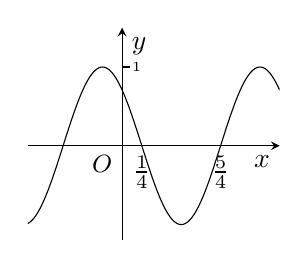
\begin{tikzpicture}
          \node[below left](O) at(0,0) {\small$\bm{O}$};
          \draw(0,1)node[right]{\tiny$1$}--(0.1,1);
          \clip(-1.2,-1.2) rectangle (2,1.5);
          \draw[->,>=stealth](-1.2,0)--(2,0) node[below left] (x){$x$};
          \draw[->,>=stealth](0,-1.2)--(0,1.5) node[below right] (y){$y$};
          \draw[domain=-1.2:2,samples=1000] plot(\x,{cos((pi*(\x)+1/4*pi) r)});
          \node[below] (A)at (0.25,0){$\frac{1}{4}$};
          \node[below] (B)at (1.25,0){$\frac{5}{4}$};
        \end{tikzpicture}
      \end{minipage}
      \begin{answer}
        D
      \end{answer}
    \item 《2018天利38套:高考真题单元专题训练(理)ISBN978-7-223-03438-8》专题15三角恒等变换 P57p4【2008•山东】\\
      (2008 \textbullet {\kaishu 山东})已知$\cos{\Bigl(\alpha-\dfrac{\piup}6\Bigr)}+\sin\alpha=\dfrac{4}5\sqrt{3}}$,则$\sin{\Bigl(\alpha+\dfrac{7\piup}6\Bigr)}$的值是\xz
      \xx{$-\dfrac{2\sqrt{3}}5$}
       {$\dfrac{2\sqrt{3}}5$}
       {$-\dfrac{4}5$}
       {$\dfrac{4}5$}
      \begin{answer}
        C
      \end{answer}
    \item 《2018天利38套:高考真题单元专题训练(理)ISBN978-7-223-03438-8》专题15三角恒等变换 P57p5【2014•全国新课标】\\
      (2014 \textbullet {\kaishu 全国新课标})设$\alpha\in\Bigl(0,\dfrac{\piup}2\Bigr)$,$\beta\in\Bigl(0,\dfrac{\piup}2\Bigr)$,且$\tan\alpha=\dfrac{1+\sin\beta}{\cos\beta}$,则\xz
      \xx{$3\alpha-\beta=\dfrac{\piup}2$}
       {$3\alpha+\beta=\dfrac{\piup}2$}
       {$2\alpha-\beta=\dfrac{\piup}2$}
       {$2\alpha+\beta=\dfrac{\piup}2$}
      \begin{answer}
        C
      \end{answer}
    \item 《2018天利38套:高考真题单元专题训练(理)ISBN978-7-223-03438-8》专题15三角恒等变换 P57p7【2013•浙江】\\
      (2013 \textbullet {\kaishu 浙江})
      已知$\alpha\in\mathbb{R}$,$\sin\alpha+2\cos\alpha=\dfrac{\sqrt{10}}2$,则$\tan{2\alpha}=$\xz
      \xx{$\dfrac{4}3$}{$\dfrac{3}4$}{$-\dfrac{3}4$}{$-\dfrac{4}3$}
      \begin{answer}
        C
      \end{answer}
    \item 《2018天利38套:高考真题单元专题训练(理)ISBN978-7-223-03438-8》专题13三角函数的概念、... P49p7【2011•福建】\\
      (2011 \textbullet {\kaishu 福建})
      若$\tan\alpha=3$,则$\dfrac{\sin{2\alpha}}{\cos^2\alpha}$的值等于\xz
      \xx{2}{3}{4}{6}
      \begin{answer}
        D
      \end{answer}
    \item 《习题化知识清单》P72知识2-2【三角函数,恒成立、参数】\\
      不等式$\tan x>a$在$x\in\Bigl(-\dfrac{\piup}4,\dfrac{\piup}2 \Bigr)$上恒成立,则$a$的取值范围是\xz
      \xx{$(-\infty,-1]$}
        {$(-\infty,-1)$}
        {$(-\infty,1]$}
        {$(-\infty,1]$}
      \begin{answer}
        A
      \end{answer}
    \item 福州三中中学2015-2016学年高一数学第二学期期末检测.docx-9【三角函数,解析式、图像变换】\\
      (福州三中中学2015-2016学年高一数学第二学期期末检测9)将函数$y=\sin\Bigl(x-\dfrac{\piup}3\Bigr)$的图像上所有点的横坐标伸长到原来的2倍(纵坐标不变),再将所得的图像向左平移$\dfrac{\piup}3$个单位,得到的函数图像对应的解析式是\xz
      \xx{$y=\sin\dfrac x2$}
        {$y=\sin\Bigl(\dfrac x2-\dfrac{\piup}2\Bigr)$}
        {$y=\sin\Bigl(\dfrac{x}2-\dfrac{\piup}6\Bigr)$}
        {$y=\sin\Bigl(2x-\dfrac{\piup}6\Bigr)$}
      \begin{answer}
        C
      \end{answer}
    \item LaTeX-master/2018/qimo.tex-7【三角函数,解析式、图像】\\
      函数$f(x)=2\sin\left(\omega x+\varphi\right)\left(\omega>0,\abs{\varphi}<\dfrac{\pi}{2}\right)$的部分图象如图所示,则$ \omega,\varphi $的值分别是\xz
      \begin{minipage}[b]{0.7\linewidth}
        \vspace{1.5cm}
        \xx{$ 2,-\dfrac{\pi}{3}$}{$2,-\dfrac{\pi}{6} $}{$4,-\dfrac{\pi}{6} $}{$ 4,\dfrac{\pi}{3}$}
      \end{minipage}\hfill
      \begin{minipage}[h]{0.3\linewidth}
        \vspace{-1cm}
        \begin{tikzpicture}[>=latex,scale=1]
          \tikzmath{
            \a = 5*pi/12;
            \b=11*pi/12;
          }
          \draw[->](-1,0)--(4,0) node[below](x){$x$};
          \draw[->](0,-2.3)--(0,2.3) node[left](y){$y$};
          \node[below left](O) at(0,0){$\small O$};
          \draw[domain=0:pi,samples=1000] plot (\x,{2*sin((2*(\x)-pi/3) r)});
          \draw[dashed] (0,2)node[left](a){$2$}-|(\a,0)node[below](a1){$\dfrac{5\pi}{12}$} ;;
          \draw[dashed](0,-2)node[left](b){$-2$}-|(\b,0)node[above](b1){$\dfrac{11\pi}{12}$} ;
          %\draw[dashed] (0,2)-|($(5*pi/12,0)$);
        \end{tikzpicture}
      \end{minipage}
      \begin{answer}
        A
      \end{answer}
    \item LaTeX-master/sanjiaohanshu/gaokaosection.tex 11【三角函数,解析式、单调性】\\
      已知函数$f(x)=2\sin \left(\omega x+\varphi\right),\ x \inR$,\ 其中$ \omega>0,\ -\pi <\varphi\le \pi ,\  $若$f(x)$的最小正周期为$ 6\pi  $,且当$ x=\dfrac{\pi}{2} $时,$f(x)$取得最大值,则\xz
      \xx{$f(x)$在区间$ \left[-2\pi,0\right] $上是增函数}
        {$f(x)$在区间$ \left[-3\pi,-\pi \right] $上是增函数}
        {$f(x)$在区间$ \left[3\pi,5\pi \right] $上是减函数}
        {$f(x)$在区间$ \left[4\pi,6\pi \right] $上是减函数}
      \begin{answer}
        A
      \end{answer}
    \item LaTeX-master/sanjiaohanshu/gaokaosection.tex 13【三角函数,解析式、奇偶性】\\
       已知函数$f(x)=\Bigg\{\begin{aligned}
      \sin(x+a),x\le 0\\\cos (x+b),x>0
      \end{aligned}$是偶函数,则下列结论可能成立的是\xz
       \xx{$ a=\dfrac{\pi}{4},b=-\dfrac{\pi}{4}$}
        {$ a=\dfrac{2\pi}{3},b=\dfrac{\pi}{6}$}
        {$a=\dfrac{\pi}{3},b=\dfrac{\pi}{6} $}
        {$ a=\dfrac{5\pi}{6},b=\dfrac{2\pi}{3}$}
      \begin{answer}
        C
      \end{answer}
    \item 《习题化知识清单》P72知识3-3【三角函数,解析式,参数】\\
      若函数$y=2\cos(2x+\varphi)$是偶函数,且在$\left(0,\dfrac{\piup}4\right)$上是增函数,则实数$\varphi$可能是\xz
      \xx{$-\dfrac{\piup}2$}
        {0}
        {{$\dfrac{\piup}2$}}
        {$\piup$}
      \begin{answer}
        D
      \end{answer}
    \item 《习题化知识清单》P72方法2-1【三角函数,单调性】\\
      函数$\abs{\sin x}$的一个单调区间是\xz
      \xx{$\left(\dfrac{\piup}2,\piup\right)$}
        {$\left(\piup,2\piup\right)$}
        {$\left(\piup,\dfrac{3\piup}2\right)$}
        {$\left(0,\piup\right)$}
      \begin{answer}
        C
      \end{answer}
    \item 《习题化知识清单》P77单元检测10【三角函数,大小、奇偶性】\\
      定义在$\mathbb{R}$上的偶函数$f(x)$满足$f(x+1)=-\dfrac2{f(x)}(f(x)\neq0)$,且在区间$(2013,2014)$上单调递增.已知$\alpha,\beta$是锐角三角形的两个内角,则$f(\sin\alpha),f(\cos\beta)$的大小关系是\xz
      \xx{$f(\sin\alpha)<f(\cos\beta)$}
        {$f(\sin\alpha)>f(\cos\beta)$}
        {$f(\sin\alpha)=f(\cos\beta)$}
        {以上情况均有可能}
    \item 《习题化知识清单》P73知识1-1【三角函数,单调性、参数】\\
      若函数$f(x)=\sin \omega x(\omega>0)$在区间$\left[0,\dfrac{\piup}3 \right]$上单调递增,在区间$\left[ \dfrac{\piup}3,\dfrac{\piup}2 \right]$上单调递减,则$\omega$可以为\xz
      \xx{$\dfrac23$}
        {$\dfrac32$}
        {2}
        {3}
      \begin{answer}
        B
      \end{answer}
    \item 《习题化知识清单》P73知识1-3【三角函数,单调性】\\
      设函数$f(x)=\sqrt{2}\sin \left(\omega x+\varphi+\dfrac{\piup}4 \right)$$\left(\omega>0,\abs{\varphi}<\dfrac{\piup}2 \right)$的最小正周期为$\piup$,且$f(-x)=f(x)$,则\xz
      \xx{$f(x)$在$\left(0,\dfrac{\piup}2 \right)$上单调递减}
        {$f(x)$在$\left(\dfrac{\piup}4,\dfrac{3\piup}4 \right)$上单调递减}
        {$f(x)$在$\left(0,\dfrac{\piup}2 \right)$上单调递增}
        {$f(x)$在$\left(\dfrac{\piup}4,\dfrac{3\piup}4 \right)$上单调递增}
      \begin{answer}
        A
      \end{answer}
    \item 《习题化知识清单》P76单元检测6【三角函数,奇偶性】\\
      当$x=\dfrac{\piup}4$时,函数$f(x)=A\sin(x+\varphi)(A>0)$取得最小值,则函数$y=f\left(\dfrac{3\piup}4-x \right)$是\xz
      \xx{奇函数且图像关于点$\left(\dfrac{\piup}2,0 \right)$对称}
        {偶函数且图像关于点$\left(\piup,0 \right)$对称}
        {奇函数且图像关于直线$x=\dfrac{\piup}2$对称}
        {偶函数且图像关于点$\left(\dfrac{\piup}2,0 \right)$对称}
      \begin{answer}
        C
      \end{answer}
    \item 《习题化知识清单》P72知识2-1【三角函数,奇偶性】\\
      函数$y=\tan2\left(x+\dfrac{\piup}4 \right)$\xz
      \xx{是奇函数}
        {是偶函数}
        {既是奇函数又是偶函数}
        {是非奇非偶函数}
      \begin{answer}
        A
      \end{answer}
    \item 《习题化知识清单》P72知识2-2【三角函数,恒成立、参数】\\
      不等式$\tan x>a$在$x\in\left(-\dfrac{\piup}4,\dfrac{\piup}2 \right)$上恒成立,则$a$的取值范围是\xz
      \xx{$(-\infty,-1]$}
        {$(-\infty,-1)$}
        {$(-\infty,1]$}
        {$(-\infty,1]$}
    \item 《习题化知识清单》P75方法2.3【三角函数,图像】\\
      设函数$f(x)=\sin{\Bigl(2x+\dfrac{\piup}3\Bigr)}$,则下列结论正确的是\xz
      \xx{$f(x)$的图像关于直线$x=\dfrac{\piup}3$对称}
        {$f(x)$的图像关于点$\Bigl(-\dfrac{\piup}4,0\Bigr)$对称}
        {把$f(x)$的图像向左平移$\dfrac{\piup}{12}$个单位长度,得到一个偶函数的图像}
        {$f(x)$的最小正周期为$\piup$,且在$\Bigl[0,\dfrac{\piup}6 \Bigr]
        $上为增函数}
      \begin{answer}
        C
      \end{answer}
    \item 福建师大附中2016-2017高一下期末考试数学试题…….doc-9【二倍角、诱导公式】\\
     (2017 \textbullet {\kaishu 师大附中} 9)
     已知$\sin\Bp{\dfracp{}6-\alpha}=\dfrac13$,则$\cos\Bp{\dfracp{2}3+2\alpha}=$\xz
     \xx{$-\dfrac79$}
      {$-\dfrac13$}
      {$\dfrac13$}
      {$\dfrac79$}
     \begin{answer}
       A
     \end{answer}
    \item 福州三中2017高一下数学期末卷…….doc-6【二倍角、诱导公式】\\
      (2017 \textbullet {\kaishu 福州三中} 6)
      已知$\sin\Bp{\dfracp{3}2+\theta}+2\cos(\piup+\theta)=\sin(-\theta)$,则$\sin\theta\cos\theta+\cos^2\theta=$\xz
      \xx{$-\dfrac15$}
       {$\dfrac25$}
       {$\dfrac35$}
       {$1$}
      \begin{answer}
        B
      \end{answer}
    \item 福州一中学2016-2017学年高一下学期期末考试数学…….doc-7【和角公式,韦达定理】\\
      (2017 \textbullet {\kaishu 福州一中} 7)
      已知$\tan\alpha$,$\tan\beta$是方程$x^2+3\sqrt3x+4=0$的两根,$\alpha,\beta\in(0,\piup)$,则$\alpha+\beta=$\xz
      \xx{$\dfracp{}3$}
       {$\dfracp{2}3$}
       {$\dfracp{4}3$}
       {$\dfracp{}3$或$\dfracp{4}3$}
      \begin{answer}
        A
      \end{answer}
    \item 福州一中学2016-2017学年高一下学期期末考试数学…….doc-5【二倍角、半角、奇偶性、周期性】\\
        (2017 \textbullet {\kaishu 福州一中} 5)
        函数$f(x)=\dfrac12(1-\cos{2x})\cos^2x$,$x\in\mathbb{R}$是\xz
        \xx{最小正周期为$\piup$的偶函数}
         {最小正周期为$\dfracp{}2$的偶函数}
         {最小正周期为$\piup$的奇函数}
         {最小正周期为$\dfracp{}2$的奇函数}
        \begin{answer}
          B
        \end{answer}
    \item 《习题化知识清单》P90单元检测9【三角恒等变换,二次方程】\\
      已知$\tan\alpha$,$\tan\beta$是方程$x^2-3x-5=0$的两根,则$\tan{2(\alpha+\beta)}$的值为\xz
        \xx{$-\dfrac{24}{25}$}
          {$\dfrac{24}7$}
          {$-\dfrac{4}{5}$}
          {$-\dfrac{4}{3}$}
      \begin{answer}
        D
      \end{answer}
    \item 《高中数学竞赛培优教程+一试(李名德 主编)》.pdf P92-4.1-4【三角函数,复合、大小】\\
      (附加题,5分)
      已知$\theta\in[0,\piup]$,$f(x)=\sin{(\cos\theta)}$的最大值为$a$,最小值为$b$,$g(\theta)=\cos{(\sin\theta)}$的最大值为$c$,最小值为$d$,则$a,b,c,d$从小到大的顺序是\xz
      \xx{$b<d<a<c$}
        {$d<b<c<a$}
        {$b<d<c<a$}
        {$d<b<a<c$}
      \begin{answer}
        A
      \end{answer}
  \end{exercise}
  \subsection{填空题}
  \begin{exercise}{\bf 填空题}
    \item 【三角函数的概念】\\
      若角$\alpha$的终边经过点$P(1,-2)$,则$\tan{2\alpha}$的值为\tk.
      \begin{answer}
        $\dfrac43$
      \end{answer}
    \item 【诱导公式】\\
      若$\sin\Bp{\dfracp{}2+\theta}=\dfrac35$,则$\cos{2\theta}=$\tk.
      \begin{answer}
        $-\dfrac7{25}$
      \end{answer}
    \item 福州第三中中学2015-2016学年高一数学第二学期期末检测.doc-14【三角函数性质 综合判断】\\
      (2016 \textbullet {\kaishu 福州三中} 14)
      关于函数$f(x)=2\sin\Bp{2x+\dfrac{\piup}3}$($x\inR$),有下列说法:\\
      \circled{1}由$f(x_1)=f(x_2)=0$可得$x_1-x_2$必是$\piup$的整数倍;
      \circled{2}$y=f(x)$的表达式可改写为$f(x)=2\cos\Bp{2x-\dfrac{\piup}6}$;
      \circled{3}$y=f(x)$的图像关于点$\Bp{-\dfrac{\piup}6,0}$对称;
      \circled{4}$y=f(x)$的图像关于直线$x=\dfrac{7\piup}{12}$对称.\\
      其中说法正确的序号是\tk.
      \begin{answer}
        \circled{2}\circled{3}\circled{4}
      \end{answer}
    \item 福州屏东中学2016-2017学年高一下学期期末考试数学试题.doc-20【正弦曲线图像】\\
      (2017 \textbullet {\kaishu 屏东中学} 20)
      已知角$\alpha$的终边过点$P(-3,4)$.\\
      (1)求$\dfrac{\tan\alpha}{\sin(\piup-\alpha)-\cos\Bp{\dfracp12+\alpha}}$的值;\quad
      (2)若$\beta$为第三象限角,且$\tan\beta=\dfrac34$,求$\cos(2\alpha-\beta)$的值.
      \begin{answer}
        (1)$-\dfrac56$;
        (2)$\dfrac45$.
      \end{answer}
    \item 福州三中2017高一下数学期末卷…….doc-15【辅助角公式灵活应用】\\
         《2018天利38套:高考真题单元专题训练(理)ISBN978-7-223-03438-8》专题14三角函数的图像与性质 P54p16【2013•全国新课标】\\
      (2017 \textbullet {\kaishu 福州三中} 15)(2013 \textbullet {\kaishu 全国新课标})
      设当$x=\theta$时,函数$f(x)=\sin x-2\cos x$取得最大值,则$\cos\theta=$\tk.
      \begin{answer}
        $-\dfrac{2\sqrt{5}}5$
      \end{answer}
    \item 《2018天利38套:高考真题单元专题训练(理)ISBN978-7-223-03438-8》专题13三角函数的概念、...  P52p13【2012•广东】\\
      (2012 \textbullet {\kaishu 广东})
      已知函数$f(x)=2\cos{\Bigl(\omega x+\dfrac{\piup}6\Bigr)}$(其中$\omega>0$,$x\in\mathbb{R}$)的最小正周期为$10\piup$.\\
      (I)求$\omega$的值\\
      (II)设$\alpha,\beta\in\Bigl[0,\dfrac{\piup}2\Bigr]$,$f{\Bigl(5\alpha+\dfrac{5\piup}3\Bigr)}=-\dfrac{6}5$,$f{\Bigl(5\beta-\dfrac{5\piup}6\Bigr)}=\dfrac{16}{17}$,求$\cos{(\alpha+\beta)}$的值.
      \begin{answer}
        (I)$\omega=\dfrac{1}5$.
        (II)$\sin\alpha=\dfrac{3}5$,$\cos\beta=\dfrac{8}{17}$,$\cos\alpha=\dfrac{4}5$,$\sin\beta=\dfrac{15}{17}$,$\cos{(\alpha+\beta)}=-\dfrac{13}{85}$.
      \end{answer}
    \item 《2018天利38套:高考真题单元专题训练(理)ISBN978-7-223-03393-0》专题14三角函数的图像与性质P54p13【2016•全国新课标】【三角函数变换、辅助角】\\
        {\kaishu (2016 \textbullet 全国新课标)}
        函数$y=\sin x-\sqrt3\cos x$的图像可由函数$y=\sin x+\sqrt3\cos x$的图像至少向右平移\tk个单位长度得到.
        \begin{answer}
          $\dfrac{2\piup}3$
        \end{answer}
    \item 《2018天利38套:高考真题单元专题训练(理)ISBN978-7-223-03438-8》专题14三角函数的图像与性质 P54p16【2013•全国新课标】\\
      (2013 \textbullet {\kaishu 全国新课标})
      设当$x=\theta$时,函数$f(x)=\sin x-2\cos x$取得最大值,则$\cos\theta=$\tk.
      \begin{answer}
        $-\dfrac{2\sqrt{5}}5$
      \end{answer}
    \item 《2018天利38套:高考真题单元专题训练(理)ISBN978-7-223-03438-8》专题14三角函数的图像与性质 P55p19【2016•天津】\\
      (2016 \textbullet {\kaishu 天津})
      已知函数$f(x)=4\tan x\sin{\Bigl(\dfrac{\piup}2-x\Bigr)}\cos{\Bigl(x-\dfrac{\piup}3\Bigr)}-\sqrt{3}$.\\
      (I)求$f(x)$的定义域与最小正周期;\\
      (II)讨论$f(x)$在区间$\Bigl[-\dfrac{\piup}4,\dfrac{\piup}4\Bigr]$上的单调性.
      \begin{answer}
        (I)$f(x)=2\sin{\Bigl(2x-\dfrac{\piup}3\Bigr)}$,定义域:$\Bigl\{x\Bigm|x\neq \dfrac{\piup}2+k\piup,k\in\mathbb{Z}\Bigr\}$;
        最小正周期:$T=\piup$.
        (II)$f(x)$在区间$\Bigl[-\dfrac{\piup}{12},\dfrac{\piup}4\Bigr]$上单调递增,在区间$\Bigl[-\dfrac{\piup}4,-\dfrac{\piup}{12}\Bigr]$上单调递减.
      \end{answer}
    \item 《2018天利38套:高考真题单元专题训练(文)》专题13三角函数的概念……P41p2【2016文•全国新课标】【同角三角函数基本关系式、诱导公式】\\
      {\kaishu (2016文 \textbullet 全国新课标)}
      已知$\theta$是第四象限角,且$\sin\Bp{\theta+\dfracp{}4}=\dfrac35$,则$\tan\Bp{\theta-\dfracp{}4}=$\tk.
      \begin{answer}
        $-\dfrac43$
      \end{answer}
    \item 《2018天利38套:高考真题单元专题训练(理)ISBN978-7-223-03438-8》专题15三角恒等变换 P59p20【2014•广东】\\
      (2014 \textbullet {\kaishu 广东})已知函数$f(x)=A\sin{\Bigl(x+\dfrac{\piup}4\Bigr)}$,$x\in\mathbb{R}$,且$f\Bigl(\dfrac{5\piup}{12}\Bigr)=\dfrac{3}2$.\\
      (I)求$A$的值;\\
      (II)若$f(\theta)+f(-\theta)=\dfrac{3}2$,$\theta\in \Bigl(0,\dfrac{\piup}2\Bigr)$,求$f\Bigl(\dfrac{3\piup}4-\theta\Bigr)$.
      \begin{answer}
        (I)$A=\sqrt{3}$;
        (II)$f\Bigl(\dfrac{3\piup}4-\theta\Bigr)=\dfrac{\sqrt{30}}4$
      \end{answer}
    \item 《2018天利38套:全国卷高考常考基础题(理)ISBN978-7-223-03393-0》练习8 三角恒等变换 P22p15
      已知$\cos(x+2\theta)+2\sin\theta\sin(x+\theta)=\dfrac{1}3$,则$\cos{2x}$的值为\tk.
      \begin{answer}
        $-\dfrac{7}9$
      \end{answer}
    \item 《2018天利38套:高考真题单元专题训练(理)ISBN978-7-223-03438-8》专题15三角恒等变换 P58p11【2017•江苏】\\
      (2017 \textbullet {\kaishu 江苏})
      若$\tan{\Bigl(\alpha-\dfrac{\piup}4\Bigr)}=\dfrac{1}6$,则$\tan\alpha=$\tk.
      \begin{answer}
        $\dfrac{7}5$
      \end{answer}
    \item 《2018天利38套:全国卷高考常考基础题(理)ISBN978-7-223-03393-0》练习8 三角恒等变换 P22p20
      已知$\sin{2\alpha}-2=2\cos{2\alpha}$,则$\sin^2\alpha+\sin{2\alpha}=$\tk.
      \begin{answer}
        $1$或$\dfrac{8}5$
      \end{answer}
    \item 《2018天利38套:高考真题单元专题训练(理)ISBN978-7-223-03438-8》专题15三角恒等变换 P58p16【2016•上海】\\
      (2016 \textbullet {\kaishu 上海})方程$3\sin x=1+\cos{2x}$在区间$[0,2\piup]$上的解为\tk.
      \begin{answer}
        $\dfrac{\piup}6$,$\dfrac{5\piup}6$
      \end{answer}
    \item 《2018天利38套:高考真题单元专题训练(理)ISBN978-7-223-03438-8》专题15三角恒等变换 P58p17【2016•江苏】\\
      (2016 \textbullet {\kaishu 江苏})
      在锐角三角形$ABC$中,若$\sin{A}=2\sin{B}\sin{C}$,则$\tan{A}\tan{B}\tan{C}$的最小值是\tk.
      \begin{answer}
        8
      \end{answer}
    \item 《2018天利38套:高考真题单元专题训练(理)ISBN978-7-223-03438-8》专题15三角恒等变换 P59p19【2010•上海】\\
      (2010 \textbullet {\kaishu 上海})已知$0<x<\dfrac{\piup}2$,化简:\\
      $\lg\Bigl(\cos x\tan x+1-2\sin^2{\dfrac{x}2}\Bigr)+\lg\biggl[\sqrt{2}\cos {\Bigl(x-\dfrac{\piup}4\Bigr)}\biggr]-\lg(1+\sin{2x})$.
      \begin{answer}
        0
      \end{answer}
    \item 《2019金考卷双测20套(文)ISBN978-7-5371-9890-5》题型5三角函数、三角恒等变换P15p3【2018•福州期末】【三角恒等变换】\\
        {\kaishu (2018 \textbullet 福州期末(文))}
        $\sqrt3\cos15\degree-4\sin^215\degree\cos15\degree=$\xz
        \xx{$\dfrac12$}
         {$\dfrac{\sqrt2}2$}
         {$1$}
         {$\sqrt2$}
        \begin{answer}
          D
        \end{answer}
    \item 《2019金考卷双测20套(文)ISBN978-7-5371-9890-5》题型5三角函数、三角恒等变换P15p4【2018•唐山五校联考】【三角恒等变换】\\
        {\kaishu (2018 \textbullet 唐山五校联考(文))}
        已知$\alpha$是第三象限角,且$\tan\alpha=2$,则$\sin\Bp{\alpha+\dfrac{\piup}4}=$\xz
        \xx{$-\dfrac{3\sqrt{10}}{10}$}
         {$\dfrac{3\sqrt{10}}{10}$}
         {$-\dfrac{\sqrt{10}}{10}$}
         {$\dfrac{\sqrt{10}}{10}$}
        \begin{answer}
          A
        \end{answer}
    \item LaTeX-master/sanjiaohanshu/gaokaosection.tex 26【三角函数,单调性】\\
      已知函数$f(x)=\sin (2x+\varphi)$,若$    f\left(\dfrac{\piup}{12}\right)-f\left(-\dfrac{5\piup}{12}\right)=2 $,则函数$f(x)$的单调增区间为\tk.
      \begin{answer}
        $\left[k\piup-\dfrac{5\piup}{12},k\piup+\dfrac{\piup}{12}\right],k\in\mathbb{Z}$
      \end{answer}
    \item LaTeX-master/sanjiaohanshu/gaokaosection.tex 31【三角函数,图像变换,性质】\\
      把函数$ y=\sin 2x $的图象沿$x$轴向左平移$ \dfrac{\pi}{6} $个单位,纵坐标伸长到原来的2倍(横坐标不变)后得到函数$ y=f(x) $的图象,对于函数$ y=f(x) $有以下四个判断:\\
      \ding{192} 该函数的解析式为$ y=2\sin \left(2x+\dfrac{\pi}{6}\right) $;\\
      \ding{193} 该函数图象关于点$ \left(\dfrac{\pi}{3},0\right) $对称;\\
      \ding{194} 该函数在$ \left[0,\dfrac{\pi}{6}\right] $上是增函数;\\
      \ding{195} 若函数$ y=f(x)+a $在$ \left[0,\dfrac{\pi}{2}\right] $上的最小值为$ \sqrt{3},\  $则$ a=2\sqrt{3} .$\\
      其中,正确判断的序号是\tk.
      \begin{answer}
        \circled{2}\circled{3}\circled{4}
      \end{answer}
    \item 福建师大附中2015-2016学年高一数学第二学期期末检测.doc-17【诱导公式】\\
      (2016 \textbullet {\kaishu 师大附中} 17)
      已知$\sin\Bp{\theta-\dfracp{}4}=\dfrac13$,则$\cos\Bp{\dfracp{}4+\theta}$的值等于\tk.
      \begin{answer}
        $-\dfrac13$
      \end{answer}
    \item 《习题化知识清单》P70方法3.2【同角三角函数关系化简】\\
      已知$\sin\alpha\cos\alpha=-\dfrac{12}{25}$,$\alpha\in\Bigl(-\dfrac{\piup}4,0\Bigr)$,则$\sin\alpha+\cos\alpha=$\tk.
      \begin{answer}
        $\dfrac{1}{5}$
      \end{answer}
    \item 《习题化知识清单》P72例1-1【三角函数,最值】\\
      函数$\dfrac{\sin x-2}{2+\sin x}$的最大值为\tk.
      \begin{answer}
        $-\dfrac13$
      \end{answer}
    \item 《习题化知识清单》P72例1【三角函数,值域】\\
      函数$\dfrac{\sin x+2}{\sin x+1},x\in\Bigl[0,\dfrac{\piup}2\Bigr]$的值域为\tk.
      \begin{answer}
        $\Bigl[\dfrac32,2\Bigr]$
      \end{answer}
    \item 《习题化知识清单》P73易混清单例【三角函数,单调性】\\
      函数$y=2\sin\left(\dfrac{\piup}3-2x \right)$的单调增区间为\tk.
      \begin{answer}
        $\left[k\piup+\dfrac{5\piup}{12},k\piup+\dfrac{11\piup}{12} \right],k\in\mathbb{Z}$
      \end{answer}
    \item 《习题化知识清单》P74易混清单练【三角函数,单调性】\\
      函数$y=2\sin\left(\dfrac{\piup}3-2x \right)$的单调减区间为\tk.
      \begin{answer}
        $\left[k\piup+\dfrac{\piup}6,k\piup+\dfrac{2\piup}3 \right],k\in\mathbb{Z}$
      \end{answer}
    \item 《习题化知识清单》P77单元检测12【三角函数,单调性、参数】\\
      设$\omega>0$,若函数$f(x)=2\sin \omega x(\omega>0)$在区间$\left[-\dfrac{\piup}3,\dfrac{\piup}4 \right]$上单调递增,则$\omega$取值范围是\tk.
      \begin{answer}
        $\left(0,\dfrac32\right]$
      \end{answer}
    \item 《习题化知识清单》P87方法1【三角函数式化简】\\
      化简:
      $\sin{\Bigl(3x+\dfrac{\piup}3\Bigr)}\cos{\Bigl(x-\dfrac{\piup}6\Bigr)}+\cos{\Bigl(3x+\dfrac{\piup}3\Bigr)}\cos{\Bigl(x+\dfrac{\piup}3\Bigr)}=$\tk.
      \begin{answer}
        \cos{2x}
      \end{answer}
    \item 《习题化知识清单》P87方法1【三角函数式化简】\\
      函数$y=\sin{\Bigl(\dfrac{\piup}2+x\Bigr)\cos{\Bigl(\dfrac{\piup}6-x\Bigr)}}$的最大值为\tk.
      \begin{answer}
        $\dfrac{2+\sqrt{3}}4$
      \end{answer}
    \item 《习题化知识清单》P89方法1-1【三角恒等变换,函数性质】\\
      已知函数$f(x)=\dfrac{(\sin x-\cos x)\sin {2x}}{\sin x}$,则$f(x)$的单调递减区间为\tk[6].
     \begin{answer}
       $\Bigl[k\piup+\dfrac{3\piup}8,k\piup+\dfrac{7\piup}8\Bigr](k\in\mathbb{Z})$
     \end{answer}
    \item 高中数学习题解法辞典.pdf 例2-1-8【三角函数,不等式】\\
     已知$\abs{\cos \theta}\leqslant \abs{\sin\theta}$,则$\theta$的取值范围是\tk.
     \begin{answer}
       $\Bigl[k\piup+\dfrac{\piup}4,k\piup+\dfrac{3\piup}4\Bigr],k\in\mathbb{Z}$
     \end{answer}
   \item 高中数学习题解法辞典.pdf 2-1-74【三角函数,同名关系式、方程】\\
     已知$1+\sin^2x=\cos x$,则$x=$\tk.
     \begin{answer}
       $2k\piup(k\in\mathbb{Z})$
     \end{answer}
    \item 高中数学习题解法辞典.pdf 例2-1-19【三角函数,方程】\\
     已知$\sin\Bigl(\dfrac{\piup}2+2x\Bigr)=-\dfrac12$,则$x=$\tk.
     \begin{answer}
       k\piup\pm\dfrac{\piup}3(k\in\mathbb{Z})
     \end{answer}
    \item 高中数学习题解法辞典.pdf 例2-2-4【三角函数,定义域、对数】\\
     函数$y=\sqrt{25-x^2}+\lg\sin\Bigl(x+\dfrac{\piup}3\Bigr)$的定义域为\tk.
     \begin{answer}
       $\Bigl[-5,-\dfrac{4\piup}3\Bigr)\bigcup\Bigl(-\dfrac{\piup}3,\dfrac{2\piup}3\Bigr)$
     \end{answer}
    \item 函数y=Asin(ωx+φ)的图象及简单应用P11.9【三角函数,奇偶性】\\
     若$f(x)=\cos\left(2x+\dfrac{\piup}3+\varphi\right)$$(\abs{\varphi}<\dfrac{\piup}2)$是奇函数,则$\varphi=$\tk.
     \begin{answer}
       $\dfrac{\piup}6$
     \end{answer}
    \item 《高中数学奥林匹克竞赛解题方法大全(周沛耕 主编)》.pdf P93例3【三角函数,恒等变换】\\
     (附加题,5分)
     $\sqrt3\tan{18\degree}+\tan{18\degree}\tan{12\degree}+\sqrt3\tan{12\degree}=$\tk.
     \begin{answer}
       1
     \end{answer}
  \end{exercise}
  \subsection{解答题}
  \begin{exercise}{\bf 解答题}
    \item 【三角函数,化简、表达式计算】\\
      (本小题满分12分)\par
      (1)化简:$\dfrac{\cos{\Bigl(\alpha-\dfrac{\piup}2\Bigr)}}{\sin{\Bigl(\dfrac{5\piup}2+\alpha\Bigr)}}\cdot\sin{(\alpha-2\piup)}\cdot\cos{(\piup-\alpha)}$;\\
      (2)已知$\tan{a}=-2$,求$\dfrac{\sin{2a}-\cos^2{a}}{2+\cos{2a}}$的值.
      \begin{answer}
      解:(1)$\text{原式}=\dfrac{\sin\alpha}{\cos\alpha}\cdot\sin\alpha\cdot(-\cos\alpha)=-\sin^2\alpha$;\\
      (2)$\because\tan\alpha=-2$,
      $\therefore\text{原式}=\dfrac{2\sin\alpha\cdot\cos\alpha-\cos^2\alpha}{2\cos^2\alpha+1}
      =\dfrac{2\sin\alpha\cdot\cos\alpha-\cos^2\alpha}{3\cos^2\alpha+\sin^2\alpha}
      =\dfrac{\dfrac{2\sin\alpha\cdot\cos\alpha-\cos^2\alpha}{\cos^2\alpha}}{\dfrac{3\cos^2\alpha+\sin^2\alpha}{\cos^2\alpha}}
      =\dfrac{2\tan\alpha-1}{3+\tan^2\alpha}=\dfrac{2\times(-2)-1}{3+(-2)^2}
      =-\dfrac{5}{7}.$
      \end{answer}
    \item 【三角函数,数量积、恒等变换、不等式、图像变换】\\
      (本小题满分12分)\\
      设函数$f(x)=\bm a\cdot\bm b$,其中向量$\bm a=(\cos x,1)$,$\bm b=\bigl(\cos x,\sqrt3\sin x\cos x\bigr)$,$x\in\mathbb{R}$.\\
      (1)求函数$f(x)$的解析式;\\
      (2)求满足$f(x)\leqslant0$的$x$的集合;\\
      (3)函数$y=\sin x$的图像可由函数$y=f(x)$的图像经过怎样的变换得到?
      \begin{answer}
        解:(1)$f(x)=\bm a\cdot\bm b
        =\cos^2x+\sqrt3\sin x\cos x
        =\dfrac{\cos{2x}+1}2+\dfrac{\sqrt3}{2}\sin{2x}
        =\sin{\Bigl(2x+\dfrac{\piup}6\Bigr)}+\dfrac12.$\\
        (2)$\because f(x)\leqslant0$,
        $\therefore \sin{\Bigl(2x+\dfrac{\piup}6\Bigr)}\leqslant-\dfrac12.$\\
        又$\because$不等式$\sin x\leqslant-\dfrac12$的解集为$\Bigl[2k\piup-\dfrac{5\piup}6,2k\piup-\dfrac{\piup}6\Bigr],k\in\mathbb{Z}.$\\
        $\therefore 2k\piup-\dfrac{5\piup}6 \leqslant 2x+\dfrac{\piup}6 \leqslant 2k\piup-\dfrac{\piup}6$.\\
        解得:$k\piup-\dfrac{\piup}2 \leqslant x \leqslant k\piup-\dfrac{\piup}6$
        即:函数$f(x)\leqslant0$的$x$的解集为$\Bigl\{x\Bigm| k\piup-\dfrac{\piup}2 \leqslant x \leqslant k\piup-\dfrac{\piup}6,k\in\mathbb{Z}\Bigr\}$.\\
        (3)函数$y=\sin x$的图像可由函数$y=f(x)$的图像经过以下步骤变换得到:\\
        $\circled{1}$向下平移$\dfrac12$个单位,得到函数$y=\sin{\Bigl(2x+\dfrac{\piup}6\Bigr)}$的图像;\\
        $\circled{2}$向右平移$\dfrac{\piup}{12}$个单位,得到函数$y=\sin {2x}$的图像;\\
        $\circled{3}$横坐标伸长2倍,得到函数$y=\sin x$的图像.
      \end{answer}
    \item 【三角函数,恒等变换、存在性、参数】\\
      (本小题满分12分)\\
      已知函数$f(x)=2\sin^2{\Bigl(\dfrac{\piup}4+x\Bigr)}+\sqrt3\cos{2x}$.\\
      (1)求函数$f(x)$的最小正周期和对称轴方程;\\
      (2)若关于$x$的方程$f(x)-m=2$在$x\in\Bigl[0,\dfrac{\piup}2\Bigr]$上有两个不同的解,求实数$m$的取值范围.
      \begin{answer}
        【分析】(1)利用三角函数的倍角公式以及辅助角公式将函数进行化简即可求最小正周期和对称轴方程;\\
        (2)求出函数$f(x)$在$x\in\Bigl[0,\dfrac{\piup}2\Bigr]$的取值情况,利用数形结合即可得到结论.\\
        【解答】解:(1)由$f(x)=2\sin^2{\Bigl(\dfrac{\piup}4+x\Bigr)}+\sqrt3\cos{2x}
        =1-\cos{\Bigl(\dfrac{\piup}2+2x\Bigr)}+\sqrt3\cos{2x}
        =1+\sin{2x}+\sqrt3\cos{2x}=1+2\sin{\Bigl(\dfrac{\piup}3+2x\Bigr)}$,\\
        $\because \omega=2$,$\therefore$函数$f(x)$的最小正周期为$\piup$.\\
        由$2x+\dfrac{\piup}3=\dfrac{\piup}2+k\piup,k\in\mathbb{Z}$得:$x=\dfrac{\piup}{12}+\dfrac12k\piup,{k\in\mathbb{Z}}$,\\
        故函数$f(x)$的对称轴方程为:$x=\dfrac{\piup}{12}+\dfrac12k\piup,{k\in\mathbb{Z}}$.\\
        (2)由$f(x)-m=2$得$f(x)=m+2$,\\
        \begin{tikzpicture}[declare function={f(\k)=1+2*sin(deg(2*\k+pi/3));}]
          \tikzset{elegant/.style={smooth,thick,samples=50,magenta}}
          \begin{axis}[axis x line=middle,
                 axis y line=middle,
                 xmin=-1.3,xmax=2.5,
                 ymin=-1.6,ymax=3.5,
                 xstep=1,ystep=1,
                 ytick distance=1,
                 ylabel=$y$,
                 xlabel=$x$]
                \addplot[elegant,orange,domain=0:pi/2]{f(x)};
                \addplot[elegant,dashed,domain=-1.2:1.2]{3};
                \addplot[elegant,domain=-1:2]{2.732};
          \end{axis}
        \end{tikzpicture}
        当${x\in\Bigl[0,\dfrac{\piup}2\Bigr]}$时,$2x+\dfrac{\piup}3\in\Bigl[\dfrac{\piup}3,\dfrac{4\piup}3\Bigr]$,\\
        由图象得$f(0)=1+2\sin{\dfrac{\piup}3}=1+\sqrt3$,\\
        函数$f(x)$的最大值为$1+2=3$,\\
        $\therefore$要使方程$f(x)-m=2$在$x\in\Bigl[0,\dfrac{\piup}2\Bigr]$上有两个不同的解,
        则$f(x)=m+2$在$x\in\Bigl[0,\dfrac{\piup}2\Bigr]$上有两个不同的解,\\
        即函数$f(x)$和$y=m+2$在$x\in\Bigl[0,\dfrac{\piup}2\Bigr]$上有两个不同的交点,\\
        即$1+\sqrt3\leqslant m+2<3$,\\
        即 $\sqrt3-1\leqslant m<1$.
      \end{answer}
    \item 【三角函数,数量积、恒等变换、单调性、存在性、参数】\\
      (本小题满分12分)\\
      已知向量$\bm a=\Bigl(\dfrac{1}2,\sin x\Bigr)$,$\bm b=\biggl(-1,\cos{\Bigl(x-\dfrac{\piup}6\Bigr)}\biggr)$,$f(x)=\bm a\cdot\bm b+\dfrac{1}4$,$(x\in\mathbb{R})$.\\
      (1)求函数$f(x)$的单调递减区间;\\
      (2)若函数$g(x)=f(x)-m,\Bigl(\dfrac{\piup}3\leqslant x\leqslant\dfrac{13\piup}{12}\Bigr)$有两个不同的零点$x_1,x_2$,求实数$m$的取值范围及$x_1,x_2$的和.
      \begin{answer}
        解:(1)$f(x)=\bm a\cdot\bm b+\dfrac{1}4
        =-\dfrac12+\sin{x}\cdot\cos{\Bigl(x-\dfrac{\piup}6\Bigr)}+\dfrac14
        =\sin{x}\cdot \Bigl(\cos x\cos{\dfrac{\piup}6}+\sin x\sin{\dfrac{\piup}6}\Bigr)-\dfrac14
        =\dfrac{\sqrt3}2\sin x\cos x+\dfrac12\sin^2x-\dfrac14
        =\dfrac{\sqrt3}4\sin{2x}-\dfrac14\cos{2x}
        =\dfrac12\sin{\Bigl(2x-\dfrac{\piup}6\Bigr)}$.\\
        由$2x-\dfrac{\piup}6\in\Bigl[\dfrac{\piup}2+2k\piup,\dfrac{3\piup}2+2k\piup\Bigr]$,${k\in\mathbb{Z}}$,解得$x\in\Bigl[\dfrac{\piup}3+k\piup,\dfrac{5\piup}6+k\piup\Bigr]$,${k\in\mathbb{Z}}$.\\
        $\therefore$函数$f(x)$的单调递减区间为$\Bigl[\dfrac{\piup}3+k\piup,\dfrac{5\piup}6+k\piup\Bigr]$,${k\in\mathbb{Z}}$.\\
        (2) $\because$函数$g(x)=f(x)-m,\Bigl(\dfrac{\piup}3\leqslant x\leqslant\dfrac{13\piup}{12}\Bigr)$有两个不同的零点$x_1,x_2$,
        $\therefore$函数$y=f(x)$的图像与函数$y=m$的图像在$\Bigl[\dfrac{\piup}3,\dfrac{13\piup}{12}\Bigr]$上有两个交点.\\
        又$\because \dfrac{\piup}3\leqslant x\leqslant\dfrac{13\piup}{12}$,
        $\therefore 2x-\dfrac{\piup}6\in\Bigl[\dfrac{\piup}2,2\piup\Bigr]$.
      \end{answer}
    \item 福建师大附中2016-2017高一下期末考试数学试题…….doc-20【三角函数性质,向量数量积计算】\\
      (2017 \textbullet {\kaishu 师大附中} 20)
      已知向量$\bm a=(\cos x,\sin x)$,$\bm b=(3,-\sqrt3)$,记$f(x)=\bm a\cdot\bm b$.\\
      (I)求$f(x)$的单调增区间;\\
      (II)若$x\in[0,\piup]$,求$f(x)$的值域.
      \begin{answer}
        (I)$\Bigl[-\dfrac{5\piup}6+2k\piup,\dfrac{11\piup}6+2k\piup\Bigr]$,$k\inZ$;
        (II)$[-2\sqrt3,3]$.
      \end{answer}
    \item 《习题化知识清单》P77单元检测15 【三角函数,解析式、单调性】\\
      已知函数$f(x)=\sin(\omega x+\varphi)$$(\omega>0,0<\varphi<\piup)$的最的最小正周期为$\piup$,且函数$f(x)$的图像过点$\left(\dfrac{\piup}2,-1\right)$.\\
      (1)求$\omega$和$\varphi$的值;
      (2)设$g(x)=f(x)+f\left(\dfrac{\piup}4-x \right)$,求函数$g(x)$的单调递增区间.
      \begin{answer}
        (1)$\omega=2$,$\varphi=\dfrac{\piup}2$.
        (2)$\left[k\piup-\dfrac{3\piup}8,k\piup+\dfrac{\piup}8\right](k\in\mathbb{Z})$
      \end{answer}
    \item 函数y=Asin(ωx+φ)的图象及简单应用P11.14【三角函数,解析式、值域】\\
      已知曲线$y=A\sin(\omega x+\varphi)$$(A>0,\omega>0,\abs{\varphi}\leqslant\dfrac{\piup}2)$上最高点为$(2,\sqrt{2})$,该最高点与相邻的最低点间的曲线与$x$轴交于点$(6,0)$.\\
      (1)该函数的解析式;\\
      (2)该函数在$x\in[-6,0]$上的值域.
      \begin{answer}
        (1)$y=\sqrt{2}\sin(\dfrac{\piup}8x+\dfrac{\piup}4)$;
        (2)$[-\sqrt{2},0]$
      \end{answer}
    \item 福州格致中学2015-2016学年高一数学第二学期期末检测.docx-22【三角函数,解析式、存在性、参数、大小】\\
      (附加题:本小题满分15分)\\
      (福州格致中学2015-2016学年高一数学第二学期期末检测22)已知函数$f(x)=A\sin(\omega x+\varphi)+B (A>0,\omega>0)$的一系列对应值如下表:
      \begin{center}
        \renewcommand{\arraystretch}{1.4}
        \begin{tabular}{|*{8}{c|}}
          \hline
            $x$
            &$\dfrac{\piup}6$
            &$-\dfrac{\piup}3$
            &$-\dfrac{5\piup}6$
            &$-\dfrac{4\piup}3$
            &$-\dfrac{11\piup}6$
            &$-\dfrac{7\piup}3$
            &$-\dfrac{17\piup}6$\\
          \hline
            $y$
            &$-1$
            &$1$
            &$3$
            &$1$
            &$-1$
            &$1$
            &$3$\\
          \hline
        \end{tabular}\\
      \end{center}
      (1)根据表格提供的数据求函数$f(x)$的一个解析式;\\
      (2)根据(1)的结果:\\
      \;(i)当$x\in\Bigl[0,\dfrac{\piup}3\Bigr]$时,方程$f(3x)=m$恰有两个不同的解,求实数$m$的取值范围;\\
      \;(ii)若是$\alpha,\beta$是锐角三角形的两个内角,试比较$f(\sin \alpha)$与$f(\cos \beta)$的大小.
      \begin{answer}
        (1)$f(x)=2\sin\Bigl(x-\dfrac{\piup}3\Bigr)+1$;(2)(i)$[\sqrt{3}+1,3)$;(ii)易得$f(x)$在$[-\dfrac{\piup}6,\dfrac{5\piup}6]$上单调递增,故$f(x)$在$[0,1]$上单调递增;又$0<\dfrac{\piup}2-\beta<\alpha<\dfrac{\piup}2$,从而$\sin\alpha>\sin(\dfrac{\piup}2-\beta)=\cos\beta$,于是$f(\sin \alpha)>f(\cos \beta)$
      \end{answer}
    \item 福建师大附中2015-2016学年高一数学第二学期期末检测.doc-20【诱导公式,化简】\\
      (2016 \textbullet {\kaishu 师大附中} 20)
      已知$\cos\alpha=-\dfrac{\sqrt5}5$,$\alpha\in\Bp{\piup,\dfracp{3}2}$.\\
      (I)求$\sin\alpha$的值;
      (II)求$\dfrac{\sin(\piup+\alpha)+2\sin\Bp{\dfracp{3}2+\alpha}}{\cos(3\piup-\alpha)+1}$的值.
      \begin{answer}
        (I)$\sqrt5-1$
        (II)原式$=\dfrac{-\sin\alpha-2\cos\alpha}{-\cos\alpha+1}=\dfrac{\sqrt5}5+1$
      \end{answer}
    \item 福建师大附中2015-2016学年高一数学第二学期期末检测.doc-22【三角函数性质】\\
      (2016 \textbullet {\kaishu 师大附中} 22)
      已知函数$f(x)=3\sin\Bp{\dfrac{x}2+\dfrac{\piup}6}+3$,$x\inR$.\\
      (I)求函数$f(x)$的单调增区间;\\
      (II)若$x\in\Bigl[\dfrac{\piup}3,\dfrac{4\piup}3\Bigr]$,求$f(x)$的最大值和最小值,
      并指出$f(x)$取得最值时相
      应$x$的值.
      \begin{answer}
        (I)$\Bigl[-\dfrac{4\piup}3+4k\piup,\dfrac{2\piup}3+4k\piup\Bigr]$,$k\inZ$;
        (II)当$x=\dfrac{4\piup}3$时,取最小值$f(x)_{\min}=\dfrac92$;当$x=\dfrac{2\piup}3$时,取最大值$f(x)_{\max}=6$.
      \end{answer}
    \item 福州一中学2016-2017学年高一下学期期末考试数学…….doc-10【正弦曲线图像】\\
      \begin{minipage}[t]{0.7\linewidth}
        \vspace{-1.2cm}
        (2017 \textbullet {\kaishu 福州一中} 16)
        已知函数$f(x)=A\sin(\omega x+\phi)$($A>0$,$\omega>0$,$\abs{\phi}<\dfrac{\piup}2$)的部分图像如图所示,\\
        (I)求函数$f(x)$的单调递增区间;\\
        (II)将$f(x)$的图像向右平移$\dfrac{\piup}3$个单位长度,再将所得的图像上各店的横坐标缩短到原来的$\dfrac12$倍(纵坐标不变),
        得到$g(x)$的图像;当$x\in\Bp{0,\dfrac{\piup}4}$时,求$g(x)$的值域.
      \end{minipage}\hfill
      \begin{minipage}[h]{0.3\linewidth}
        % \vspace{2.7cm}
        \begin{center}
          \begin{tikzpicture}[scale=0.8]
            \coordinate[label=below left:$O$] (O) at(0,0);
            \coordinate[label=above :\small$\tfrac{\piup}3$] (t1) at(pi/3,0);
            \draw[->,>=latex](-0.2*pi,0)--(1.2*pi,0)node[below](x) {$x$};
            \draw[->,>=latex](0,-1.5)--(0,1.5)node[right](y) {\small $y$};
            \draw [domain=-0.1*pi:0.9*pi,samples=100] plot(\x,{sin((2*\x+pi/3) r)});
            \draw[densely dashed](7*pi/12,0)node[above](pi){$\tfrac{7\piup}{12}$}--++(0,-1);
            \draw[densely dashed](0,-1)node[left](min){$-\sqrt2$}--++(7*pi/12,0);
          \end{tikzpicture}
        \end{center}
      \end{minipage}
      \begin{answer}
        (I)$f(x)=\sqrt2\sin\Bp{2x+\dfrac{\piup}3}$,单调递增区间为$\Bigl[-\dfrac{5\piup}{12}+k\piup,\dfrac{\piup}{12}+k\piup\Bigr]$,$k\inZ$.
        (II)$g(x)=\sqrt2\sin\Bp{4x-\dfrac{\piup}3}$,值域:$\Bigl[-\dfrac{\sqrt6}2,\sqrt2\Bigr]$
      \end{answer}
    \item 福建师大附中2015-2016学年高一数学第二学期期末检测.doc-24【三角函数 复合函数最值】\\
      (2016 \textbullet {\kaishu 师大附中} 24)
      求函数$f(x)=3-2a\sin x-\cos^2x$的最小值.
      \begin{answer}
        $y_{\min}=\begin{cases}
          2a+3,\quad a\leqslant-1,\\
          a^2+2,\quad -1<a<1,\\
          -2a+3,\quad a\geqslant+3.
        \end{cases}$
      \end{answer}
    \item 高中数学习题解法辞典.pdf 例2-2-1【三角函数,解析式,图像变换】\\
      已知函数$f(x)=A\sin(\omega x+\varphi)(A,\omega,\varphi\text{为常数},\omega>0)$的图像上相邻两个最高点的坐标分别是$\Bigl(\dfrac{\piup}{12},2\Bigr)$,$\Bigl(\dfrac{13\piup}{12},2\Bigr)$.\\
      (1) 求函数$f(x)$的一个表达式;\\
      (2) 画出函数$f(x)$在长度为一个周期的闭区间上的简图;\\
      (3) 说明经过怎样的变换,可以由$y=\sin x$的图像得到$y=f(x)$的图像.
      \begin{answer}
        (1)$y=2\sin\Bigl(2x+\dfrac{\piup}3\Bigr)(\varphi=k\piup-\dfrac{2\piup}3$即可);
        (2)略;
        (3)将$y=\sin x$图像上所有点向左平移$\dfrac{\piup}3$个单位得到$y=\sin \Bigl(x+\dfrac{\piup}3\Bigr)$的图像;
        再把$y=\sin \Bigl(x+\dfrac{\piup}3\Bigr)$的图像上所有点的横坐标缩短到原来的$\dfrac12$(纵坐标不变),得到$y=\sin \Bigl(2x+\dfrac{\piup}3\Bigr)$的图像;
        最后把$y=\sin \Bigl(2x+\dfrac{\piup}3\Bigr)$的图像上所有点的纵坐标伸长到原来的2倍(横坐标不变),即可得到函数$y=f(x)$的图像.
      \end{answer}
    \item 高中数学习题解法辞典.pdf 例2-2-9【三角函数,证明、周期函数、奇偶性、单调性】\\
      已知函数$y=f(x)$的定义域为$\mathbb{R}$,若$f(x+2)=-f(x)$,且当$-1\leqslant x\leqslant 1$时,$f(x)=x$,求证:\\
      (1)函数$y=f(x)$是最小正周期为4的周期函数;\\
      (2)函数$y=f(x)$是奇函数;\\
      (3)当$x\in[4k-1,4k+1](k\in\mathbb{Z})$时,$y=f(x)$是增函数;当$x\in[4k+1,4k+3](k\in\mathbb{Z})$时,$y=f(x)$是减函数.
      \begin{answer}
        (1)(提示:易证4为函数的一个周期;再用反证法证明4是最小正周期:设最小正周期$T$,且$0<T<4$,则$f(T)=f(0)=0$.分类讨论$0<T\leqslant 1$时,$1<T\leqslant 3$时,$3<T<4$时,三种情况都将推出矛盾,于是得证)
        (2)任取$x\inR$,$x$可表示为$x=2k+x'$,其中$-1\leqslant x'\leqslant 1$,$k\inZ$.于是由$f(x+2)=-f(x)$及$y=f(x)$的周期性可得:
        \[f(x)=f(2k+x')=
          \begin{cases}
            -f(x')=-x'\quad(k\text{为奇数})\\
            f(x')=x'\quad(k\text{为偶数})
          \end{cases}
        \]
        注意到$-1\leqslant x'\leqslant 1$,$-1\leqslant -x'\leqslant 1$,又有
        \[f(-x)=f(-2k-x')=
          \begin{cases}
            -f(-x')=x'\quad(k\text{为奇数})\\
            f(-x')=x'\quad(k\text{为偶数})
          \end{cases}
        \]
        综上所述,无论$k$为奇数或偶数,对于$x\inR$,总有$f(-x)=-f(x)$,故$y=f(x)$是奇函数.
        (3)(提示:利用$f(x)=f(4k+x')=f(x')=x'$,其中$-1\leqslant x'\leqslant 1$,$k\inZ$.)
      \end{answer}
    \item 高中数学习题解法辞典.pdf 2-2-44【三角函数,最值、周期应用】\\
      已知函数$f(x)=2\sin\Bigl(\omega x+\dfrac{\piup}6\Bigr)+1(\omega>0)$,\\
      (1)求$f(x)$的最大值$M$,最小值$m$以及最小正周期$T$;\\
      (2)试求最小正整数$\omega$,使得自变量$x$在任意两个整数间(包括整数本身)变化时,函数$f(x)$至少有一个值是$M$,另一个值是$m$.
      \begin{answer}
        (1)$M=3,m=-1,T=\dfrac{2\piup}{\omega}$;
        (2)$\dfrac{2\piup}{\omega}\leqslant 1$,$\omega=7$(周期为无理数,由“无理数无法表示为两整数之比”这一事实可得任一区间$[k,k+1]$,$k\inZ$内函数图像均不相同.由此,半周期必须不小于1才能满足题意)
      \end{answer}
    \item 高中数学习题解法辞典.pdf 2-2-45【三角函数,周期函数、证明】\\
      求证:(1)$f(x)=\sin x\cos x$的最小正周期为$\piup$;\\
      (2)若函数$y=f(x)(x\in\mathbb{R})$的最小正周期为$T$,则$f(kx)(k>0)$的最小正周期为$\dfrac{T}k$.
      \begin{answer}
        (1)(提示:若$0<T<\piup$,令$x=0$,得$T=\dfrac{\piup}2$,不符);(2)(提示:$f\biggl[k\Bigl(x+\dfrac{T}k\Bigr)\biggr]=f(kx+T)=f(kx)$)
      \end{answer}
    \item 福州第三中中学2015-2016学年高一数学第二学期期末检测.doc-15【诱导公式,和角】\\
      (2016 \textbullet {\kaishu 福州三中} 15)
      已知$\sin\BP{\alpha+\dfrac{\piup}4}=-\dfrac35$,且$0<\alpha<\dfrac{5\piup}4$,求$\cos\BP{\alpha+\dfrac{\piup}2}$的值.
      \begin{answer}
        $-\dfrac{\sqrt2}{10}$
      \end{answer}
    \item 福州三中2017高一下数学期末卷…….doc-17【三角函数化简、二倍角、诱导公式】\\
        (2017 \textbullet {\kaishu 福州三中} 17)
        已知$f(x)=2\tan x+\dfrac{1-2\sin^2{\dfrac{x}2}}{\sin\dfrac{x}2\cdot\cos\dfrac{x}2}$.\\
        (I)求$f(\dfrac{\piup}6)$的值;\\
        (II)若$f(\alpha)=5$,求$f\Bp{\alpha+\dfrac{\piup}4}$的值.
        \begin{answer}
          (I)$\dfrac{8\sqrt3}3$;
          (II)$\pm\dfrac{20}3$.
        \end{answer}
    \item 《2018天利38套:高考真题单元专题训练(理)ISBN978-7-223-03393-0》专题14三角函数的图像与性质P54p18【2017•山东】【正弦曲线解析式,三角恒等变换】\\
          {\kaishu (2017 \textbullet 山东)}
          设函数$f(x)=\sin\Bp{\omega x-\dfrac{\piup}6}+\sin\Bp{\omega x-\dfrac{\piup}2}$,其中$0<\omega<3$.已知$f\Bp{\dfrac{\piup}6}=0$.\\
          (I)求$\omega$;\\
          (II)将函数$y=f(x)$的图像上各点的横坐标伸长为原来的2倍(纵坐标不变),再将得到的图像向左平移$\dfrac{\piup}4$个单位,得到函数$y=g(x)$的图像,求$g(x)$在$\Bigl[-\dfrac{\piup}4,\dfrac{3\piup}4\Bigr]$上的最小值.
          \begin{answer}
            (I)$f(x)=\sqrt3\sin\Bp{\omega x-\dfrac{\piup}3}$,$\omega=2$.
            (II)$g(x)=\sqrt3\sin\Bp{x-\dfrac{\piup}{12}}$,当$x=-\dfrac{\piup}4$时,$g(x)$取得最小值$-\dfrac32$
          \end{answer}
    \item 【三角函数,模型、最值】【清大期末模拟卷18QdB4-FinExam.tex】\\
      (本小题满分12分)\\
      如图,某污水处理厂要在一个矩形污水处理池($ABCD$)的池底水平铺设污水净化管道($Rt\triangle{FHE}$,$H$是直角顶点)米处理污水,管道越长,污水净化效果越好。设计要求管道的接口$H$是$AB$的中点,$E$、$F$分别落在线段$BC$、$AD$上.已知$AB=20$米,$AD=10\sqrt3$米,记$\angle{BHE}=\theta$.\\
      (1)试将污水净化管道的长度$l$表示为$\theta$的函数,并写出定义域;\\
      (2)若$\sin\theta+\cos\theta=\sqrt2$,求此时管道的长度$l$;\\
      (3)当$\theta$取何值时,污水净化效果好?并求出此时管道的长度.\\
      \begin{flushleft}
        \begin{tikzpicture}
          \coordinate[label=left:$A$](A)at(0,0);
          \coordinate[label=right:$B$](B)at(4,0);
          \coordinate[label=left:$D$](D)at(0,3.5);
          \coordinate[label=right:$C$](C)at(4,3.5);
          \draw[dashed] (A)rectangle(C);
          \coordinate[label=below:$H$](H)at(2,0);
          \coordinate[label=right:$E$](E)at(4,3);
          \path[name path=AD] (A)--(D);
          % \coordinate (P)at($(H)!2!90:(E)$);
          \path[name path=PH] ($(H)!1!90:(E)$)--(H);
          \path[name intersections={of=AD and PH}];
          \coordinate[label=left:$F$] (F)  at (intersection-1);
          % \draw[red] ($(H)!6pt!(E)$)--($(H)!6pt!(E)!6pt!90:(E)$)--($(H)!6pt!(F)$);
          \draw \rAm{E}{H}{F};
          % \draw [--] ($(H)+(0.5,0)$) arc (0:30:1cm);
          % \node at ($(H)+(0.8,0.3)$) {$\theta$};
          % \pic["\alpha",draw=red,angle radius=0.5cm] {angle=A--B--C};
          \path (B)--(H)--(E) pic [draw,"$\theta$",angle eccentricity=1.5] {angle=B--H--E};
          \draw (H)--(E)--(F)--cycle;
        \end{tikzpicture}
      \end{flushleft}
      \begin{answer}
        解:
      \end{answer}
  \end{exercise}
\section{平面向量}
  \subsection{判断题}
  \begin{exercise}{\textbf{判断题}}
    \item 【平面向量,概念】\\
      判断下列结论是否正确(请在括号中打“\checkmark”或“\XSolidBrush”)\\
      (1)向量与有向线段是一样的,因此可以用有向线段来表示向量.(  )\\
      (2)$\abs{\bm{a}}$与$\abs{\bm{b}}$是否相等与$\bm{a}$,$\bm{b}$的方向无关.(  )\\
      (3)若$\bm{a}\varparallel\bm{b}$,$\bm{b}\varparallel\bm{c}$,则$\bm{a}\varparallel\bm{c}$.(  )\\
      (4)若向量$\vv{AB}$与向量$\vv{CD}$是共线向量,则$A,B,C,D$四点在一条直线上.(  )\\
      (5)若向量$\vv{AB}$与向量$\vv{CD}$平行,则直线$AB$与$CD$平行.(  )\\
      (6)若向量$\bm a$与任一向量$\bm b$平行,则$\bm a=\bm 0$.(  )\\
      (7)若两个向量共线,则其方向必定相同或相反.(  )
      \begin{answer}
        (2)(5)正确
      \end{answer}
    \item 【平面向量,概念】\\
      有下列命题:
      \circled{1}两个相等向量,它们的起点相同,终点也相同;
      \circled{2}若$\abs{\bm{a}}=\abs{\bm{b}}$,则$\bm{a}=\bm{b}$;
      \circled{3}若$\abs{\vv{AB}}=\abs{\vv{CD}}$,则四边形$ABCD$是平行四边形;
      \circled{4}若$\bm{m}=\bm{n}$,$\bm{n}=\bm{k}$,则$\bm{m}=\bm{k}$;
      \circled{5}位移、速率、重力加速度都是向量;
      \circled{6}共线的向量,若起点不同,则终点一定不同.其中,错误的个数是\xz
      \xx{2}{3}{4}{5}
      \begin{answer}
        D
      \end{answer}
    \item 1平面向量的基本概念.pdf P2-训练1【平面向量,概念】\\
      判断下列结论是否正确(请在括号中打“\checkmark”或“\XSolidBrush”)\\
      (1)向量就是有向线段.(  )\\
      (2)如果$\abs{\vv{AB}}>\abs{\vv{CD}}$,那么$\vv{AB}>\vv{CD}$.(  )\\
      (3)力、速度和质量都是向量.(  )\\
      (4)若$\bm a$,$\bm b$都是单位向量,则$\bm a=\bm b$.(  )\\
      (5)若$\bm a=\bm b$,且$\bm a$与$\bm b$的起点相同,则终点也相同.(  )\\
      (6)零向量的大小为0,没有方向.(  )
      \begin{answer}
        (5)正确,其余皆误.
      \end{answer}
    \item 【平面向量,概念】\\
      给出下列命题:
      \ding{192}两个具有公共终点的向量,一定是共线向量;
      \ding{193}两个向量不能比较大小,但它们的模能比较大小;
      \ding{194}$\lambda\bm{a}=\bm{0}$($\lambda$为实数),则$\lambda$必为零;
      \ding{195}$\lambda$,$\mu$为实数,若$\lambda\bm{a}=\mu\bm{b}$,则$\bm{a}$与$\bm{b}$共线.
      其中正确的命题的个数为\xz
      \xx{1}{2}{3}{4}
      \begin{answer}
        A
      \end{answer}
    \item 1平面向量的基本概念.pdf P10-训练1【平面向量,共线定理】\\
      判断下列结论是否正确(请在括号中打“\checkmark”或“\XSolidBrush”)\\
      (1)若向量$\bm b$与向量$\bm{a}$共线,则存在唯一的实数$ \lambda $,使得$\bm{b}=\lambda\bm{a}$.(\hspace{2em})\\
      (2)若$\bm{b}=\lambda\bm{a}$,则$\bm a$与$\bm b$共线.(\hspace{2em})\\
      (3)若$\lambda\bm a=\bm 0$,则$\bm a=\bm 0$.(\hspace{2em})\\
  \end{exercise}
  \subsection{选择题}
  \begin{exercise}{\bf 选择题}
    \item 【平面向量,相等】\\
      (2018·安徽淮北第一中学最后一卷)设$\bm{a}$,$\bm{b}$都是非零向量,下列四个条件,使$\dfrac{\bm{a}}{\abs{\bm{a}}}=\dfrac{\bm{b}}{\abs{\bm{b}}}$成立当且仅当\xz
      \xx{$\bm a=\bm b$}
      {$\bm a=2\bm b$}
      {$\bm a\varparallel\bm b$且$\abs{\bm a}=\abs{\bm b}$}
      {$\bm a\varparallel\bm b$且方向相同}
      \begin{answer}
        D
      \end{answer}
    \item 【向量的线性运算】\\
      若点$D$在$\triangle{ABC}$的边$BC$上,且$\vv{CD}=4\vv{DB}=r\vv{AB}+s\vv{AC}$,则$3r+s$的值为\xz
      \xx{$\dfrac{16}5$}
       {$\dfrac{12}5$}
       {$\dfrac{8}5$}
       {$\dfrac{4}5$}
      \begin{answer}
        C
      \end{answer}
    \item 1平面向量的基本概念.pdf P13-4【平面向量,表示】\\
      已知$AM$ 是$\triangle ABC$ 的边$BC$ 上的中线,若$\vv{AB}=\bm a$,$\vv{AC}=\bm b$,则$\vv{AM}$等于\xz
      \xx{$\dfrac12(\bm a-\bm b)$}
        {$-\dfrac12(\bm a-\bm b)$}
        {$\dfrac12(\bm a+\bm b)$}
        {$-\dfrac12(\bm a+\bm b)$}
      \begin{answer}
        C
      \end{answer}
    \item 《习题化知识清单》P81知识4-1【向量共线】\\
      已知向量$\bm a$、$\bm b$不共线,$\bm c=k\bm a+\bm b({k\in\mathbb{R}})$,$\bm d=\bm a-\bm b$。如果$\bm c\varparallel \bm d$,那么\xz
      \xx{$k=1$且$\bm c$与$\bm d$同向}
        {$k=1$且$\bm c$与$\bm d$反向}
        {$k=-1$且$\bm c$与$\bm d$同向}
        {$k=-1$且$\bm c$与$\bm d$反向}
      \begin{answer}
        D
      \end{answer}
    \item 《习题化知识清单》P81知识4-3【向量共线】\\
      已知向量$\bm a$、$\bm b$,且$\vv{AB}=\bm a+2\bm b$,$\vv{BC}=-5\bm a+6\bm b$,$\vv{CD}=7\bm a-2\bm b$,则一定共线的三点是\xz
      \xx{$A$、$B$、$D$}
        {$A$、$B$、$C$}
        {$B$、$C$、$D$}
        {$A$、$C$、$D$}
      \begin{answer}
        A
      \end{answer}
    \item 《习题化知识清单》P81知识4-4【向量线性运算、向量共线】\\
      已知向量$\bm a=\bm e_1+2\bm e_2$,$\bm b=2\bm e_1-\bm e_2$,则$\bm a+2\bm b$与$2\bm a-\bm b$\xz
      \xx{一定共线}
        {一定不共线}
        {当且仅当$\bm e_1$与$\bm e_2$共线时共线}
        {当且仅当$\bm e_1=\bm e_2$时共线}
      \begin{answer}
        C
      \end{answer}
    \item 《习题化知识清单》P82知识2-1【向量坐标运算】\\
      设平面向量$\bm a=(3,5)$,$\bm b=(-2,1)$,则$\bm a-2\bm b=$\xz
      \xx{(7,3)}{(7,7)}{(1,7)}{(1,3)}
      \begin{answer}
        A
      \end{answer}
    \item 《习题化知识清单》P82知识2-2【向量坐标运算,单位向量】\\
      已知$\bm a=(3,4)$,则与$\bm a$同向的单位向量的坐标是\xz
      \xx{$(3,4)$}
       {$(-\dfrac{3}5,\dfrac{4}5)$}
       {$(-\dfrac{3}5,-\dfrac{4}5)$}
       {$(\dfrac{3}5,\dfrac{4}5)$}
      \begin{answer}
        D
      \end{answer}
    \item 《习题化知识清单》P82知识3-1【向量共线】\\
      设向量$\bm a=(m,1)$,$\bm b=(1,m)$,如果$\bm a$与$\bm b$共线且方向相反,那么$m$的值为\xz
      \xx{$1$}{$-1$}{$\pm 1$}{$0$}
      \begin{answer}
        B
      \end{answer}
    \item 《习题化知识清单》P82知识3-3【向量共线,三角函数的定义】\\
      若$\bm a=\Bigl(\dfrac{3}2,\sin\alpha\Bigr)$,$\bm b=\Bigl(\sin\alpha,\dfrac{1}3\Bigr)$,且$\bm a\varparallel \bm b$,则锐角$\alpha$为\xz
      \xx{30\degree}{45\degree}{60\degree}{75\degree}
      \begin{answer}
        B
      \end{answer}
    \item 《习题化知识清单》P83知识1-1【数量积的定义、性质】\\
      在$\triangle{ABC}$中,$AB=BC=2$,$\angle{B}=\dfrac{\piup}4$,$AD$是边$BC$上的高,则$\vv{AD}\cdot\vv{AC}$的值为\xz
      \xx{0}{2}{4}{8}
      \begin{answer}
        B
      \end{answer}
    \item 《习题化知识清单》P83知识1-2【数量积的定义、性质】\\
      已知$\triangle{ABC}$中,$AB=AC=BC=6$,平面内一点$M$满足$\vv{BM}=\dfrac{2}3\vv{BC}-\dfrac{1}3\vv{BA}$,则$\vv{AC}\cdot\vv{MB}$等于\xz
      \xx{$-9$}{$-18$}{$12$}{$18$}
      \begin{answer}
        B
      \end{answer}
    \item 《习题化知识清单》P83知识2-2【向量的夹角】\\
      已知$\abs{\bm a}=2$,$\abs{\bm b}=4$,且$(\bm a+\bm b)\perp \bm a$,则$\bm a$与$\bm b$的夹角为\xz
      \xx{$\dfrac{2\piup}3$}
       {$\dfrac{\piup}3$}
       {$\dfrac{4\piup}3$}
       {$-\dfrac{2\piup}3$}
      \begin{answer}
        A
      \end{answer}
    \item 《习题化知识清单》P84知识4-2【数量积的坐标表示】\\
      已知$\bm a=(2,-3)$,$\bm b=(1,-2)$,且$\bm c\perp \bm a$,$\bm b\cdot\bm c=1$,则$\bm c$的坐标为\xz
      \xx{$(3,-2)$}{$(3,2)$}{$(-3,-2)$}{$(-3,2)$}
      \begin{answer}
        C
      \end{answer}
    \item 《习题化知识清单》P84知识4-3【数量积的坐标表示】\\
      在以$OA$为一边,$OB$为一条对角线的矩形中,$\vv{OA}=(-3,1)$,$\vv{OB}=(-2,k)$,则实数$k=$\xz
      \xx{$4\sqrt{3}$}{$3\sqrt{3}$}{$\dfrac{\sqrt{3}}2$}{$4$}
      \begin{answer}
        D
      \end{answer}
    \item 福州屏东中学2016-2017学年高一下学期期末考试数学试题.doc-4【向量共线】\\
      (2017 \textbullet {\kaishu 屏东中学} 4)
      若$A(-1,1)$,$B(1,3)$,$C(x,5)$,且$\vv{AB}=\lambda\vv{BC}$,则实数$\lambda$等于\xz
      \xx{1}{2}{3}{4}
      \begin{answer}
        1
      \end{answer}
    \item 福建师大附中2016-2017高一下期末考试数学试题…….doc-3【向量投影,坐标表示】\\
      (2017 \textbullet {\kaishu 师大附中} 3)
      若$\bm a=(2,1)$,$\bm b=(3,4)$,则向量$\bm b$在向量$\bm a$方向上的投影为\xz
      \xx{$2\sqrt5$}
       {$2$}
       {$\sqrt5$}
       {$10$}
      \begin{answer}
        A
      \end{answer}
    \item 【向量表示】【2018届贵州遵义航天高级中学一模】\\
      (2018届贵州遵义航天高级中学一模)如图所示,向量$\vv{OA}=\bm{a}$,$\vv{OB}=\bm{b}$,$\vv{OC}=\bm{c}$,$A$,$B$,$C$在一条直线上,且$\vv{AC}=3\vv{BC}$,则\xz
      \begin{minipage}[b]{0.7\linewidth}
        \xx{$\bm{c}=\dfrac32\bm{b}-\dfrac12\bm{a}$}
          {$\bm{c}=\dfrac32\bm{a}-\dfrac12\bm{b}$}
          {$\bm{c}=-\bm{a}+2\bm{b}$}
          {$\bm{c}=\bm{a}+2\bm{b}$}
      \end{minipage}\hfill
      \begin{minipage}[htbp!]{0.3\linewidth}
        \begin{center}
        \begin{tikzpicture}
          \coordinate[label=left:$O$](O)at(0,0);
          \coordinate[label=right:$C$](C)at(3,0);
          \coordinate[label=left:$A$](A)at(-1,2.5);
          \coordinate[label=right:$B$](B)at($(A)!0.66!(C)$);
          \draw (A)--(B)--(C)--cycle;
          \draw[->,>=latex] (O)--(C);
          \draw[->,>=latex] (O)--(A);
          \draw[->,>=latex] (O)--(B);
        \end{tikzpicture}
        \end{center}
      \end{minipage}
      \begin{answer}
        A
      \end{answer}
    \item 【向量表示】\\
      设$D$为$\triangle{ABC}$所在平面内一点,$\vv{BD}=3\vv{CD}$,则\xz
      \xx{$\vv{AD}=-\dfrac13\vv{AB}+\dfrac43\vv{AC}$}
       {$\vv{AD}=\dfrac43\vv{AB}-\dfrac13\vv{AC}$}
       {$\vv{AD}=\dfrac23\vv{AB}-\dfrac12\vv{AC}$}
       {$\vv{AD}=-\dfrac12\vv{AB}+\dfrac32\vv{AC}$}
      \begin{answer}
        D
      \end{answer}
    \item 【向量夹角、模长】\\
      已知$|\bm a|=1$,$\bm a\cdot\bm b=\dfrac12$,$|\bm a-\bm b|^2=1$,则$\bm a$与$\bm b$的夹角等于\xz
      \xx{30\degree}{45\degree}{60\degree}{120\degree}
      \begin{answer}
        C
      \end{answer}
    \item 【向量共线】\\
      已知向量$\bm a=(2,3)$,$\bm b=(-1,2)$,若$m\bm a+4\bm b$与$\bm a-2\bm b$共线,则$m$的值为\xz
      \xx{$\dfrac12$}{$2$}{$-\dfrac12$}{$-2$}
      \begin{answer}
        D
      \end{answer}
    \item LaTeX-master/xiangliang/xiangliangsorting.tex 练习P7-10【向量共线、线性运算】\\
      设$ D $为$\triangle ABC$所在平面内一点,$ \vv{BC}=3\vv{CD} $,则\xz
      \xx{$ \vv{AD}=-\dfrac{1}{3}\vv{AB}+\dfrac{4}{3}\vv{AC}$}
        {$ \vv{AD}=\dfrac{1}{3}\vv{AB}-\dfrac{4}{3}\vv{AC}$}
        {$ \vv{AD}=\dfrac{4}{3}\vv{AB}+\dfrac{1}{3}\vv{AC}$}
        {$ \vv{AD}=\dfrac{4}{3}\vv{AB}-\dfrac{1}{3}\vv{AC}$}
      \begin{answer}
        A
      \end{answer}
    \item 【向量的线性运算】【2017广东深圳二模】\\
      (2017 \textbullet {\kaishu 广东深圳二模})如图所示,正方形$ABCD$中,$M$是$BC$的中点,若$\vv{AC}=\lambda\vv{AM}+\mu\vv{BD}$,则$\lambda+\mu$等于\xz
      \xx{$\dfrac{4}3$}
       {$\dfrac{5}3$}
       {$\dfrac{15}8$}
       {$2$}
      \begin{center}
        \begin{tikzpicture}
          \coordinate[label=left:$A$](A)at(0,0);
          \coordinate[label=right:$B$](B)at(3.5,0);
          \coordinate[label=left:$D$](D)at(0,3.5);
          \coordinate[label=right:$C$](C)at(3.5,3.5);
          \coordinate[label=right:$M$](M)at($(B)!0.5!(C)$);
          \draw (A)--(B)--(C)--(D)--cycle;
          \draw[->,>=latex] (A)--(C);
          \draw[->,>=latex] (A)--(M);
          \draw[->,>=latex] (B)--(D);
        \end{tikzpicture}
      \end{center}
      \begin{answer}
        B
      \end{answer}
    \item 福州一中学2016-2017学年高一下学期期末考试数学…….doc-3【向量共线】\\
      (2017 \textbullet {\kaishu 福州一中} 3)
      已知向量$\bm a$,$\bm b$不共线,且$\bm c=\lambda\bm a+\bm b$,$\bm d=\bm a+(2\lambda-1)\bm b$,若$\bm c$与$\bm d$方向相反,则实数$\lambda$的值为\xz
      \xx{$1$}
       {$-\dfrac12$}
       {$1$或$-\dfrac12$}
       {$-1$或$-\dfrac12$}
      \begin{answer}
        B
      \end{answer}
    \item 福州格致中学2015-2016学年高一数学第二学期期末检测.docx-8【向量共线】\\
      (2016 \textbullet {\kaishu 格致中学} 8)
      设$\bm e_1$,$\bm e_2$是两个不共线的向量,$\vv{AB}=2\bm e_1+k\bm e_2$,$\vv{CB}=2\bm e_1+3\bm e_2$,$\vv{CD}=2\bm e_1-\bm e_2$,若$A$,$B$,$D$三点共线,则$k=$\xz
      \xx{$\dfrac12$}
        {$-8$}
        {$-\dfrac18$}
        {$2$}
      \begin{answer}
        B
      \end{answer}
    \item 福州三中2017高一下数学期末卷…….doc-5【向量投影,基底表示】\\
      (2017 \textbullet {\kaishu 福州三中} 5)
      设$\bm e_1$,$\bm e_2$为单位向量,且$\bm e_1$,$\bm e_2$的夹角为$\dfrac{\piup}3$,若$\bm a=\bm e_1-3\bm e_2$,$\bm b=\bm e_1+\bm e_2$,则向量$\bm a$在$\bm b$方向上的射影为\xz
      \xx{$-\sqrt3$}
       {$\sqrt3$}
       {$-\dfrac{\sqrt{10}}5$}
       {$\dfrac{\sqrt{10}}5$}
      \begin{answer}
        A
      \end{answer}
    \item 【平面向量,几何应用】\\
      已知四边形$ABCD$ 是菱形,则下列等式中成立的是\xz
      \xx{$\vv{AB}+\vv{BC}=\vv{CA}$}
        {$\vv{AB}+\vv{AC}=\vv{BC}$}
        {$\vv{AC}+\vv{BA}=\vv{AD}$}
        {$\vv{AC}+\vv{AD}=\vv{DC}$}
      \begin{answer}
        C
      \end{answer}
    \item 【向量坐标法在平面几何的应用,三角函数定义】\\
      %如图,
      半径为$\sqrt{3}$的扇形$AOB$的圆心角为120\degree,点$C$在$\arc{AB}$上,且$\angle{COB}=30\degree$,若$\vv{OC}=\lambda\vv{OA}+\mu\vv{OB}$,则$\lambda+\mu$等于\xz
      \xx{$\sqrt{3}$}
       {$\dfrac{\sqrt{3}}3$}
       {$\dfrac{4\sqrt{3}}3$}
       {$2\sqrt{3}$}
      \begin{answer}
        A
      \end{answer}
    \item 【平面向量几何应用:垂直问题】\\
      直角坐标系$xOy$中,$\vv{AB}=(2,1)$,$\vv{AC}=(3,k)$,若$\triangle{ABC}$是直角三角形,则$k$的可能值个数是\xz
      \xx{1}{2}{3}{4}
      \begin{answer}
        B
      \end{answer}
    \item 福建师大附中2016-2017高一下期末考试数学试题…….doc-6【数量积,三角形形状】\\
      (2017 \textbullet {\kaishu 师大附中} 6)
      若点$O$是$\triangle{ABC}$平面内一点,且满足$(\vv{OB}-\vv{OC})\cdot(\vv{OB}+\vv{OC}-2\vv{OA})=0$,则$\triangle{ABC}$形状为\xz
      \xx{钝角三角形}{等腰三角形}{直角三角形}{锐角三角形}
      \begin{answer}
        B
      \end{answer}
    \item 《习题化知识清单》P85方法3-4.1【向量夹角垂直】\\
      向量$\bm a=(1,-2),\bm b=(2,1)$,则\xz
      \xx{$\bm a\varparallel \bm b$}
        {$\bm a\perp \bm b$}
        {$\bm a$与$\bm b$的夹角为$60\degree$}
        {$\bm a$与$\bm b$的夹角为$30\degree$}
      \begin{answer}
        B
      \end{answer}
    \item 《习题化知识清单》P84知识5-23【数量积应用,三角形五心】\\
      点$O$是$\triangle{ABC}$所在平面上的一点,且满足$\vv{OA}\cdot\vv{OB}=\vv{OB}\cdot\vv{OC}=\vv{OA}\cdot\vv{OC}$,则点$O$是$\triangle{ABC}$的\xz
        \xx{重心}
          {垂心}
          {内心}
          {外心}
      \begin{answer}
        B
      \end{answer}
    \item 《习题化知识清单》P90单元检测8【向量投影】\\
      在平面直角坐标系中,$AB=CD$,$A(0,3)$,$B(-4,0)$,$C(a,-1)(a>0)$,则向量$\vv{BC}$在$\vv{AB}$上的投影为\xz
        \xx{$-5$}
          {$-3$}
          {$3$}
          {$5$}
      \begin{answer}
        A
      \end{answer}
    \item 《习题化知识清单》P90单元检测10【数量积;三角恒等变换,综合】\\
      已知向量$\bm a=\Bigl(\cos\dfrac{3x}2,\sin\dfrac{3x}2\Bigr)$,$\bm b=\Bigl(\cos\dfrac{x}2,-\sin\dfrac{x}2\Bigr)$,且$x\in\Bigl[0,\dfrac{\piup}2\Bigr]$,
      若$\abs{\bm a+\bm b}=2\bm a\cdot\bm b$,则$\sin{2x}+\tan{x}=$\xz
      \xx{$-1$}{$0$}{$2$}{$-2$}
      \begin{answer}
        B
      \end{answer}
    \item 《高中数学竞赛培优教程+一试(李名德 主编)》.pdf P122-5.2-3【平面向量,表示】\\
      (附加题,5分)
      已知正方形$PQRS$对角线交点为$M$,坐标原点$O$不在正方形内部,$\vv{OP}=(0,3)$,$\vv{OS}=(4,0)$,则向量$\vv{RM}$为\xz
      \xx{$\Bigl(-\dfrac{7}{2},-\dfrac{1}{2}\Bigr)$}
        {$\Bigl(\dfrac{7}{2},\dfrac{1}{2}\Bigr)$}
        {$(7,4)$}
        {$\Bigl(\dfrac{7}{2},\dfrac{7}{2}\Bigr)$}
      \begin{answer}
        A
      \end{answer}
  \end{exercise}
  \subsection{填空题}
  \begin{exercise}{\bf 填空题}
    \item 【平面向量,线性运算】
      \begin{enumerate}[label=\arabic*)]
        \item $3(6\bm{a}+\bm{b})-9(\bm{a}+\dfrac13\bm{b})=$\tk;
        \item 若$2(\bm{y}-\dfrac13\bm{a})-\dfrac12(\bm c+\bm b-3\bm y)+\bm b=0$其中$\bm a$,$\bm b$,$\bm c$为已知向量,则未知向量$\bm y=$\tk.
        \item 若$\bm a=\bm b+\bm c$,化简$3(\bm a+2\bm b)-2(3\bm b+\bm c)-2(\bm a+\bm b)=$\tk.
      \end{enumerate}
      \begin{answer}
        (1)$9\bm a$;(2)$\dfrac4{21}\bm a-\dfrac17\bm b+\dfrac17\bm c$;$-\bm a$.
      \end{answer}
    \item 【平面向量,共线定理】\\
      设向量$\bm a$,$\bm b$不共线,向量$\lambda\bm a+\bm b$与$\bm a+2\bm b$共线,则实数$\lambda=$\tk.
      \begin{answer}
        $\dfrac12$
      \end{answer}
    \item 【平面向量,表示】\\
      如图,在$\triangle ABC$中,$D$,$E$为边$AB$的两个三等分点,$\vv{CA}=3\bm a$,$\vv{CB}=2\bm b$,求$\vv{CD}$,$\vv{CE}$(用$\bm a$,$\bm b$表示).
      \begin{flushright}
        \begin{tikzpicture}
          \coordinate[label=left:$B$](B)at(0,0);
          \coordinate[label=right:$C$](C)at(2.5,0);
          \coordinate[label=above:$A$](A)at(3,3);
          \coordinate[label=above:$E$](E)at($(B)!0.33!(A)$);
          \coordinate[label=above:$D$](D)at($(B)!0.66!(A)$);
          \draw (A)--(B)--(C) --cycle;
          \draw (C)--(D) (C)--(E);
          \draw[->,>=latex] (C)--(A);
          \draw[->,>=latex] (C)--(B);
        \end{tikzpicture}
      \end{flushright}
      \begin{answer}
        $\vv{CD}=2\bm a+\dfrac23\bm b$;$\vv{CE}=\bm a+\dfrac43\bm b$
      \end{answer}
    \item 【平面向量,夹角】\\
      正方形$ABCD$中,向量$\vv{AC}$与$\vv{BC}$的夹角为\tk,向量$\vv{AC}$与$\vv{CD}$的夹角为\tk.
      \begin{answer}
        \dfrac{\piup}4(45\degree);\dfrac{3\piup}4(135\degree)
      \end{answer}
    \item 【平面向量,轨迹】\\
      在平面内,若将所有单位向量的起点平移到同一点,则它们的终点构成的图形为\tk.
      \begin{answer}
        单位圆
      \end{answer}
    \item 【平面向量,加减】\\
      如图,$\vv{AB}+\vv{BC}-\vv{AD}$等于\xz
      \begin{minipage}[b]{0.7\linewidth}
      	\xx{$\vv{AD}$}{$\vv{DC}$}{$\vv{DB}$}{$\vv{AB}$}
      \end{minipage}\hfill
      \begin{minipage}[h]{0.3\linewidth}
        \begin{tikzpicture}
          \coordinate[label=left:$B$](B)at(0,0);
          \coordinate[label=right:$C$](C)at(3,0);
          \coordinate[label=above:$A$](A)at(1.5,2);
          \coordinate[label=below:$D$](D)at($(B)!0.4!(C)$);
          \draw (A)--(B)--(C)--cycle;
          \draw (A)--(D);
        \end{tikzpicture}
      \end{minipage}
      \begin{answer}
        B
      \end{answer}
    \item 《习题化知识清单》P82知识1-3【平面向量基本定理】\\
      已知向量$\bm a=(1,2)$,$\bm b=(-2,3)$,$\bm c=(4,1)$,若用$\bm a$和$\bm b$表示$\bm c$,则$\bm c=$\tk.
      \begin{answer}
        $2\bm a-\bm b$
      \end{answer}
    \item 《习题化知识清单》P82知识2-3【向量坐标运算,中点坐标公式】\\
      已知平面直角坐标系$xOy$内的三点分别是$A(2,-5)$,$B(3,4)$,$C(-1,-3)$,$D$为线段$BC$的中点,
      则向量$\vv{DA}$的坐标为\tk.
      \begin{answer}
        $(1,-\dfrac{11}2)$
      \end{answer}
    \item 《习题化知识清单》P82知识3-4【向量共线坐标表示】\\
      若向量$\vv{OA}=(k,6)$,$\vv{OB}=(4,5)$,$\vv{OC}=(1-k,10)$,且$A$,$B$,$C$三点共线,则$k=$\tk.
      \begin{answer}
        $\dfrac{17}6$
      \end{answer}
    \item 《习题化知识清单》P82知识2-4【向量的投影】\\
      已知点$A(-1,1)$,$B(1,2)$,$C(-2,-1)$,$D(3,4)$,则向量$\vv{CD}$在$\vv{AB}$方向上的投影为\tk.
      \begin{answer}
        $3\sqrt{5}$
      \end{answer}
    \item 《习题化知识清单》P83方法2【向量共线条件应用】\\
      平面内给定三个向量$\bm a=(3,2)$,$\bm b=(-1,2)$,$\bm c=(4,1)$,则\\
      (1)若$(\bm a+k\bm c)\varparallel(2\bm b-\bm a)$,则实数$k=$\tk;\\
      (2)设$\bm d=(x,y)$满足$(\bm d-\bm c) \varparallel (\bm a+\bm b)$且$\abs{\bm d-\bm c}=1$,则$\bm d=$\tk.
      \begin{answer}
        (1)$k=-\dfrac{16}{13}$;(2)$\bm d=\Bigl(\dfrac{20+\sqrt{5}}5,\dfrac{5+2\sqrt{5}}5\Bigr)$或$\Bigl(\dfrac{20-\sqrt{5}}5,\dfrac{5-2\sqrt{5}}5\Bigr)$
      \end{answer}
    \item 《习题化知识清单》P83方法2-2【向量共线条件应用】\\
      若平面向量$\bm a$,$\bm b$满足$\abs{\bm a+\bm b}=1$,$\bm a+\bm b$平行于$x$轴,$\bm b=(2,-1)$,则$\bm a=$\tk.
      \begin{answer}
        $(-1,1)$或$(-3,1)$
      \end{answer}
    \item 《习题化知识清单》P84方法1-1【向量夹角,参数】\\
       已知$\abs{\bm a}=1,\abs{\bm b}=2$,$\bm a$与$\bm b$的夹角为$120\degree$,则使$\bm a+k\bm b$与$k\bm a+\bm b$的夹角为锐角的实数$k$的取值范围是\tk[5].
      \begin{answer}
        $\Bigl(\dfrac{5-\sqrt{21}}2,1\Bigr)\bigcup\Bigl(1,\dfrac{5+\sqrt{21}}2\Bigr)$
      \end{answer}
    \item 《习题化知识清单》P84方法2【求向量模的基本方法】\\
      已知向量$\bm a$,$\bm b$夹角为45\degree,且$\abs{\bm a}=1$,$\abs{2\bm a-\bm b}=\sqrt{10}$,则$\abs{\bm b}=$\tk.
      \begin{answer}
        $3\sqrt{2}$
      \end{answer}
    \item 《习题化知识清单》P84方法2-4【求向量模的基本方法】\\
      已知向量$\bm a=(x.y)$,$\bm b=(-1,2)$,且$\bm a+\bm b=(1,3)$,则$\abs{\bm a-2\bm b}$等于\tk.
      \begin{answer}
        $8\sqrt{2}$
      \end{answer}
    \item 《习题化知识清单》P84知识3-3【数量积的运算律】\\
      已知不共线向量$\bm a$,$\bm b$,$\abs{\bm a}=2$,$\abs{\bm b}=3$,$\bm a\cdot(\bm b-\bm a)=1$,则$\abs{\bm b-\bm a}=$\tk.
      \begin{answer}
        $\sqrt{3}$
      \end{answer}
    \item 《习题化知识清单》P84知识5-3【数量积的应用,运算律】\\
      已知$\abs{\bm a}=\abs{\bm b}=1$,$\bm a$,$\bm b$的夹角是直角,
      $\bm c=2\bm a+3\bm b$,$\bm d=k\bm a-4\bm b$,$\bm c\perp\bm d$,则$k=$\tk.
      \begin{answer}
        6
      \end{answer}
      已知$\triangle{ABC}$是正三角形,若$\vv{AC}-\lambda\vv{AB}$与向量$\vv{AC}$的夹角大于90\degree,则实数$\lambda$的取值范围是\tk.
      \begin{answer}
        $(2,+\infty)$
      \end{answer}
    \item 《习题化知识清单》P85方法4【数量积,数形结合】\\
      在矩形$ABCD$中,$AB=\sqrt{2}$,$BC=2$,点$E$为$BC$的中点,点$F$在边$CD$上,若$\vv{AB}\cdot\vv{AF}=\sqrt{2}$,则$\vv{AE}\cdot\vv{BF}$的值是\tk.
      \begin{answer}
        $\sqrt{2}$
      \end{answer}
    \item 《习题化知识清单》P85方法4-5.2【数量积,数形结合】\\
      已知正方形$ABCD$的边长为1,点$E$是$AB$边上的动点,则$\vv{DE}\cdot\vv{CB}$的值为\tk;$\vv{DE}\cdot\vv{DC}$的最大值为\tk.
      \begin{answer}
        1;1
      \end{answer}
    \item 《高中数学竞赛培优教程+一试(李名德 主编)》.pdf P121-例5.19【平面向量,不等式、数形结合】\\
      已知$x^2+y^2=25$,函数$z=\sqrt{8y-6x+50}+\sqrt{8y+6x+50}$的最大值为\tk.
      \begin{answer}
        $z_{\max}=6\sqrt{10}$(当且仅当$x=0$,$y=5$时取得)
      \end{answer}
    \item 福州三中2017高一下数学期末卷…….doc-16【向量投影,基底表示】\\
     (2017 \textbullet {\kaishu 福州三中} 16)
     已知$\bm a$,$\bm b$是平面内两个相互垂直的单位向量,若向量$\bm c$满足$(\bm a-\bm c)\cdot(\bm b-\bm c)=0$,则$|\bm c|$的最大值是\tk.
     \begin{answer}
       $\sqrt2$
     \end{answer}
    \item 福建师大附中2016-2017高一下期末考试数学试题…….doc-15【向量夹角,线性运算模长】\\
     (2017 \textbullet {\kaishu 师大附中} 15)
     已知单位向量$\bm a$,$\bm b$的夹角为$\dfracp{}3$,那么$|\bm a-2\bm b|=$\tk.
     \begin{answer}
       $\sqrt3$
     \end{answer}
    \item 【平面向量的模与夹角】\\
     已知$\triangle{ABC}$是正三角形,若$\vv{AC}-\lambda\vv{AB}$与向量$\vv{AC}$的夹角大于90\degree,则实数$\lambda$的取值范围是\tk.
     \begin{answer}
       $(2,+\infty)$
     \end{answer}
    \item 【向量几何应用】\\
     在平面四边形$ABCD$中,若$AC=3$,$BD=2$,则$(\vv{AB}+\vv{DC})\cdot(\vv{AC}+\vv{BD})=$\tk.
     \begin{answer}
       5
     \end{answer}
    \newline
    {\begin{minipage}[b]{0.65\linewidth}
      \item LaTeX-master/xiangliang/xiangliangsorting.tex P10-p48【向量表示】\\
      在$\triangle ABC$中,点$ M$,$N $满足$ \vv{AM}=2\vv{MC}$,$\vv{BN}=\vv{NC}$.若$\vv{MN}=x\vv{AB}+y\vv{AC}$,则$ x= $\tk;$ y= ~$ \tk.
      \begin{answer}
        $x=\dfrac12$;$y=-\dfrac16$
      \end{answer}
     \end{minipage}
     \begin{minipage}[htbp!]{0.3\linewidth}
       \begin{center}
       \begin{tikzpicture}
         \draw(0,0)node[below](B){\small$B$}--(1,0)node[below](N){\small$N$}--(2,0)node[below](C){\small$C$};
         \draw (0,0)--(1.1,2.1)node[above](A){\small$A$}--(2,0);
         \draw (1,0)--(1.1,2.1);
         \draw(1,0)--($(1.1,2.1)!0.7!(2,0)$)node[right](M){\small$M$};
       \end{tikzpicture}
       \end{center}
     \end{minipage}}
    \item 福建师大附中2016-2017高一下期末考试数学试题…….doc-17【数量积,几何】\\
     (2017 \textbullet {\kaishu 师大附中} 17)
     在$\triangle{ABC}$中,$|\vv{AD}|=|\vv{BD}|=|\vv{CD}|$,$|\vv{AB}|=3$,则$\vv{AB}\cdot\vv{AD}=$\tk.
     \begin{answer}
       $\dfrac92$
     \end{answer}
    \item 【向量坐标法在平面几何的应用,直线方程】\\
     在$\mathrm{Rt}\triangle{ABC}$中,$CA=CB=2$,$M$,$N$是斜边$AB$上的两个动点,且$MN=\sqrt{2}$,则$\vv{CM}\cdot\vv{CN}$的取值范围是\tk.
     \begin{answer}
       $\Bigl[\dfrac{3}2,2\Bigr]$
     \end{answer}
    \item 福州一中学2016-2017学年高一下学期期末考试数学…….doc-14【数量积,外心】\\
     (2017 \textbullet {\kaishu 福州一中} 14)
     $\triangle{ABC}$中,$CA=4$,$CB=6$,点$O$为$\triangle{ABC}$的外心,则$\vv{CO}\cdot\vv{AB}=$\tk.
     \begin{answer}
       5
     \end{answer}
  \end{exercise}
  \subsection{解答题}
  \begin{exercise}{\bf 解答题}
    \item 【平面向量,表示】\\
      如图所示,在五边形$ABCDE$中,若四边形$ACDE$是平行四边形,且$\vv{AB}=\bm{a}$,$\vv{AC}=\bm{b}$,$\vv{AE}=\bm{c}$,试用向量$\bm a$,$\bm b$,$\bm c$表示向量$\vv{BD}$,$\vv{BC}$,$\vv{BE}$,$\vv{CD}$及$\vv{CE}$.
      \begin{flushright}
        \begin{tikzpicture}
          \coordinate[label=left:$D$](D)at(0,0);
          \coordinate[label=right:$E$](E)at(3,0);
          \coordinate[label=above:$C$](C)at(1,1.5);
          \coordinate[label=below:$A$](A)at($(C)+(E)$);
          \coordinate[label=below:$B$](B)at(3.5,2.5);
          \draw (A)--(B)--(C)--(D)--(E) --cycle;
          \draw (B)--(D) (B)--(E) (C)--(E);
          \draw[->,>=latex] (A)--(B);
          \draw[->,>=latex] (A)--(C);
          \draw[->,>=latex] (A)--(E);
        \end{tikzpicture}
      \end{flushright}
      \begin{answer}
        $\vv{BD}=-\bm a+\bm c+\bm b$;$\vv{BC}=\bm b-\bm a$;$\vv{BE}=\bm a-\bm a$;$\vv{CD}=\bm c$;$\vv{CE}=\bm c-\bm b$.
      \end{answer}
    \item 1平面向量的基本概念.pdf P13-10【平面向量,加减、计算】\\
      化简:\\
      \circled{1} $\vv{BC}+\vv{AB}$; \hspace{2em} \circled{2} $\vv{DB}+\vv{CD}+\vv{BC}$;\\
      \circled{3} $\vv{AB}-\vv{FD}+\vv{CD}-\vv{CB}+\vv{FA}$;\hspace{2em} \circled{4} $(\vv{AC}+\vv{BO}+\vv{OA})-(\vv{DC}-\vv{DO}-\vv{OB})$;\\
      \begin{answer}
        \circled{1}$\vv{AC}$;\circled{2}$\bm 0$;\circled{3}$\bm 0$;\circled{4}$\bm 0$
      \end{answer}
    \item 1平面向量的基本概念.pdf P8训练5【平面向量,模型】\\
      一架飞机从$A$ 地按北偏东$35\degree$的方向飞行800 km 到达$B$ 地接到受伤人员,然后又从$B$ 地按南偏东$55\degree$的方向飞行600 km 送往$C $地医院,求这架飞机飞行的路程及两次位移的和.
      \begin{answer}
        路程1400km,位移1000km.
      \end{answer}
    \item 1平面向量的基本概念.pdf P3训练3【平面向量,模型】\\
      一辆汽车从$A $点出发向西行驶了100 km 到达$B $点,然后又改变方向向西偏北$50\degree$走了200 km到达$C$ 点,最后又改变方向,向东行驶了100 km 到达$D$ 点.\\
      (1)作出向量$\vv{AB}$,$\vv{BC}$,$\vv{CD}$;\\
      (2)求$\abs{\vv{AD}}$.
    \item 1平面向量的基本概念.pdf P10例2 【平面向量,共线定理、三点共线、证明】\\
      设$\bm a$,$\bm b$是不共线的两个非零向量.\\
      (1)若$\vv{OA}=2\bm a-\bm b$,$\vv{OB}=3\bm a+\bm b$,$\vv{OC}=\bm a-3\bm b$,求证:$A$,$B$,$C$三点共线;\\
      (2)若$8\bm a+k\bm b$与$k\bm a+\2\bm b$共线,求实数$k$的值;\\
      (3)若$\vv{OM}=m\bm a$,$\vv{ON}=n\bm b$,$\vv{OP}=\alpha\bm a+\beta\bm b$,其中$m$,$n$,$\alpha$,$\beta$均为实数,且$m,n\neq 0$,若$M$,$P$,$N$三点共线,求证:$\dfrac{\alpha}m+\dfrac{\beta}n=1$
      \begin{answer}
        (1)$\because \vv{AB}=\bm a+2\bm b$,$\vv{CB}=2\bm a+4\bm b$;$\therefore \vv{CB}=2\vv{AB}$;
        (2)$k=2\sqrt2$;
      \end{answer}
    \item 【平面向量;几何、证明】\\
      设点$G$为$\triangle ABC$重心,$D$,$E$,$F$分别为各边中点.试用向量证明:$AG=\dfrac23 AD$.
      \begin{flushright}
        \begin{tikzpicture}
          \coordinate[label=left:$B$](B)at(0,0);
          \coordinate[label=right:$C$](C)at(3,0);
          \coordinate[label=above:$A$](A)at(2,2);
          \coordinate[label=below:$D$](D)at($(B)!0.5!(C)$);
          \coordinate[label=right:$E$](E)at($(A)!0.5!(C)$);
          \coordinate[label=above:$F$](F)at($(B)!0.5!(A)$);
          \coordinate[label=above:$G$](G)at($(D)!0.33!(A)$);
          \draw (A)--(B)--(C) --cycle;
          \draw (A)--(D) (B)--(E) (C)--(F);
        \end{tikzpicture}
      \end{flushright}
    \item 【平面向量;几何、证明】\\
      设点$G$为$\triangle ABC$重心,$D$,$E$,$F$分别为各边中点.\\
      (1)试用向量证明:三角形三条中线共点;
      (2)求$\vv{AD}+\vv{BE}+\vv{CF}$.
      \begin{flushright}
        \begin{tikzpicture}
          \coordinate[label=left:$B$](B)at(0,0);
          \coordinate[label=right:$C$](C)at(3,0);
          \coordinate[label=above:$A$](A)at(2,2);
          \coordinate[label=below:$D$](D)at($(B)!0.5!(C)$);
          \coordinate[label=right:$E$](E)at($(A)!0.5!(C)$);
          \coordinate[label=above:$F$](F)at($(B)!0.5!(A)$);
          \coordinate[label=above:$G$](G)at($(D)!0.33!(A)$);
          \draw (A)--(B)--(C) --cycle;
          \draw (A)--(D) (B)--(E) (C)--(F);
        \end{tikzpicture}
      \end{flushright}
    \item 【平面向量;三点共线、证明】\\
      已知$\vv{OA}=\lambda\vv{OB}+\mu\vv{OC}$($\lambda,\mu\in\mathbb{R}$),若$\lambda+\mu=1$,求证:点$A$,$B$,$C$三点共线.
    \item 【平面向量;几何、证明】\\
      【定比分点坐标公式】如图,设$P$为$\triangle ABO$边$AB$上一点.设$\vv{OA}=\bm a$,$\vv{OB}=\bm b$\vspace{8pt}\\
      (1)求证:$\vv{OP}=\dfrac{\abs{\vv{PB}}}{\abs{\bm b-\bm a}}\bm a+\dfrac{\abs{\vv{PA}}}{\abs{\bm b-\bm a}}\bm b$;\vspace{8pt}\\
      (2)设$\vv{AP}=\lambda\vv{PB}$,求证:$\vv{OP}=\dfrac{\bm a+\lambda\bm b}{1+\lambda}$\\
      \begin{flushright}
        \vspace{-4cm}
        \begin{tikzpicture}
          \coordinate[label=left:$O$](O)at(0,0);
          \coordinate[label=right:$A$](A)at(3,0);
          \coordinate[label=above:$B$](B)at(2,2);
          \coordinate[label=right:$P$](P)at($(B)!0.4!(A)$);
          \draw (A)--(B)--(O) --cycle;
          \draw[->,>=latex] (O)--(A);
          \draw[->,>=latex] (O)--(B);
          \draw[->,>=latex] (O)--(P);
        \end{tikzpicture}
      \end{flushright}
    \item 【平面向量,夹角、模】\\
      (本小题满分10分)求值:\\
      已知$\abs{\vv a}=\sqrt2,\abs{\vv{\mathstrut b}}=1$\\
      (1)若$\vv a,\vv b$的夹角$\theta$为$45\degree$,求$\abs{\vv{\mathstrut a}-\vv{\mathstrut b}}$;\\
      (2)若$(\vv{\mathstrut a}-\vv{\mathstrut b})\perp \vv{\mathstrut b}$,求$\vv{\mathstrut a}$与$\vv{\mathstrut b}$的夹角$\theta$.
      \begin{answer}
        解:(1) $\abs{\vv a-\vv b}=\sqrt{\vv a^2-2\vv a\!\cdot\!\vv b+\vv b^2}=\sqrt{2-2\times\sqrt2\times1\times\dfrac{\sqrt2}2+1}=1$\fz[5]
        (2)$\because(\vv a-\vv b)\perp\vv b$,\\
        $\therefore(\vv a-\vv b)\cdot\vv b=\vv a\cdot\vv b-\vv b^2=\sqrt2\times1\times\cos\theta-1=0$,\\
        $\therefore\cos\theta=\dfrac{\sqrt2}2(0\le\theta\le\piup)$,$\therefore\theta=\dfrac{\piup}4.$\fz[10]
      \end{answer}
    \item 《习题化知识清单》P91单元检测16【三点共线,向量共线】\\
      设两个非零向量$\bm a$与$\bm b$不共线\\
      (1)若$\vv{AB}=\bm a+\bm b$,$\vv{BC}=2\bm a+8\bm b$,$\vv{CD}=3(\bm a-\bm b)$,求证:$A$,$B$,$D$三点共线;\\
      (2)试确定实数$k$,使$k\bm a+\bm b$与$\bm a+k\bm b$共线.
      \begin{answer}
        (1)略;(2)$k=\pm1$
      \end{answer}
    \item 福州屏东中学2016-2017学年高一下学期期末考试数学试题.doc-17【向量共线】\\
      (2017 \textbullet {\kaishu 屏东中学} 17)
      已知向量$\bm m=(\cos\alpha,1-\sin\alpha)$,$\bm n=(-\cos\alpha,\sin\alpha)$($\alpha\inR$)\\
      (I)若$\bm m\perp\bm n$,求角$\alpha$的值;\qquad (II)若$\abs{\bm m-\bm n}=\sqrt3$,求$\cos{2\alpha}$的值.
      \begin{answer}
        (I)$\alpha=\dfrac{\piup}2$
        (II)$\cos{2\alpha}=\dfrac{\sqrt2}2$
      \end{answer}
    \item 福建师大附中2016-2017高一下期末考试数学试题…….doc-19【向量共线、夹角、模长】\\
      (2017 \textbullet {\kaishu 师大附中} 19)
      已知$\bm a$,$\bm b$为两个不共线向量,$\abs{\bm a}=2$,$\abs{\bm b}=1$,$\bm c=2\bm a-\bm b$,$\bm d=\bm a+k\bm b$.\\
      (I)若$\bm c\varparallel\bm d$,求实数$k$;\\
      (II)若$k=-7$,且$\bm c\perp\bm d$,求$\bm a$与$\bm b$的夹角.
      \begin{answer}
        (I)$k=-\dfrac12$
        (II)$\vangle{\bm a}{\bm b}=\dfrac{\piup}3$
      \end{answer}
    \item 福州一中学2016-2017学年高一下学期期末考试数学…….doc-15【数量积,垂直】\\
      (2017 \textbullet {\kaishu 福州一中} 15)
      已知$\bm a=(\cos\alpha,k\sin\alpha)$,$\bm b=(\cos\beta,\sin\beta)$($k>0$,$0<\alpha<\beta<\dfrac{\piup}2$),且$\bm a+\bm b$与$\bm a-\bm b$相互垂直.\\
      (1)求$k$的值;\\
      (2)若$\bm a\cdot\bm b=\dfrac45$且$\cos\beta=\dfrac35$,求$\sin\alpha$的值.
      \begin{answer}
        (1)$k=1$;
        (2)$\sin\alpha=\dfrac7{25}$
      \end{answer}
    \item 【平面向量基本定理】\\
      在$\triangle{OAB}$的边$OA$,$OB$上分别取点$M$,$N$,使得$\vv{OA}=3\vv{OM}$,$\vv{OB}=4\vv{ON}$,设线段$AN$与$BM$交于点$P$,
      记$\vv{OA}=\bm a$,$\vv{OB}=\bm b$,用$\bm a$,$\bm b$表示向量$\vv{OP}$.
      \begin{answer}
        $\vv{OP}=\dfrac3{11}\bm a+\dfrac3{11}\bm b$
      \end{answer}
    \item 【平面向量基本定理】\\
      在$\triangle{OAB}$中,$\vv{OA}=4\vv{OC}$,$\vv{OB}=2\vv{OD}$,设线段$AD$与$BC$交于点$M$,
      记$\vv{OA}=\bm a$,$\vv{OB}=\bm b$.\\
      (1)用$\bm a$,$\bm b$表示向量$\vv{OP}$.\\
      (2)已知在线段$AC$上取一点$E$,在线段$BD$上取一点$F$,使$EF$过点$M$,设$\vv{OE}=p\vv{OA}$,$\vv{OF}=q\vv{OA}$,求证$\dfrac1{7p}+\dfrac3{7q}=1$
      \begin{answer}
        (1)$\vv{OP}=\dfrac17\bm a+\dfrac37\bm b$
        (2)略
      \end{answer}
    \item 【向量垂直】\\
      平面向量$\bm a=(\sqrt{3},-1)$,$\bm=\Bp{\dfrac12,\dfrac{\sqrt3}2}$,若存在不同时为0的实数$k$和$t$,使$\bm x=\bm a+(t^2-3)\bm b$,$\bm y=-k\bm a+t\bm b$,且$\bm x\perp\bm y$,试求函数关系式$k=f(t)$.
      \begin{answer}
        $k=f(t)=\dfrac14(t^3-3t)$
      \end{answer}
    \item 福州三中2017高一下数学期末卷…….doc-18【向量垂直,模长,共线】\\
      (2017 \textbullet {\kaishu 福州三中} 18)
      平面内的向量$\bm a=(3,2)$,$\bm b=(-1,2)$,$\bm c=(4,1)$.\\
      (I)若$(\bm a+k\bm c)\perp(2\bm b-\bm a)$,求实数$k$的值;\\
      (II)若向量$\bm d$满足$\bm d\varparallel\bm c$,且$\abs{\bm d}=\sqrt{34}$,求向量$\bm d$的坐标.
      \begin{answer}
        (I)$k=-\dfrac{11}{18}$
        (II)$\bm d=(4\sqrt2,\sqrt2)$或$\bm d=(-4\sqrt2,-\sqrt2)$
      \end{answer}
    \item 《高中数学竞赛培优教程+一试(李名德 主编)》.pdf P115-例5.10【平面向量,数量积、垂直、平行】\\
      已知向量$\bm a=(\cos\alpha,\sin\alpha)$,$\bm b=(\cos\beta,\sin\beta)$,且$\bm a$,$\bm b$满足关系$\abs{k\bm a+\bm b}=\sqrt{3}\abs{\bm a-k\bm b}$($k>0$).\\
      (1)求将$\bm a$与$\bm b$的数量积用$k$表示的解析式$f(k)$;\\
      (2)\hspace{5pt}$\bm a$能否和$\bm b$垂直?$\bm a$能否和$\bm b$平行?若不能,则说明理由;若能,则求出对应的$k$值;\\
      (3)求$\bm a$与$\bm b$夹角的最大值.
      \begin{answer}
        (1)$f(k)=\dfrac{k^2+1}{4k} (k>0)$;
        (2)$\bm a$与$\bm b$不可能垂直;当$k=2\pm\sqrt{3}$时,$\bm a\varparallel \bm b$;
        (3)60\degree
      \end{answer}
    \item 《高中数学竞赛培优教程+一试(李名德 主编)》.pdf P114-例5.8【平面向量,垂直、模长】\\
      已知$\bm a=(\cos\alpha,\sin\alpha)$,$\bm b=(\cos\beta,\sin\beta)$($0<\alpha<\beta<\piup$).\\
      (1)求证:$\bm a+\bm b$与$\bm a-\bm b$相互垂直;\\
      (2)若$k\bm a+\bm b$与$\bm a-k\bm b$大小相等,求$\beta-\alpha$(其中$k$为非零实数).
      \begin{answer}
        (1)略;(2)$\dfrac{\piup}2$
      \end{answer}
    \item 《高中数学竞赛培优教程+一试(李名德 主编)》.pdf P118-例5.14【平面向量,最值、夹角】【2004年湖北高考题】\\
      (2004年湖北高考题)在$\mathrm{Rt}\triangle{ABC}$中,已知$BC=a$,若长为$2a$的线段$PQ$以点$A$为中点,问$\vv{PQ}$与$\vv{BC}$的夹角$\theta$取何值时$\vv{BP}\cdot\vv{CQ}$的值最大?并求出这个最大值.
      \begin{answer}
        $\theta=0$时,$\vv{BP}\cdot\vv{CQ}$取最大值0.
      \end{answer}
    \item 【平面向量,表示】\\
      已知点$P$是$\triangle{ABC}$内一点,且满足条件$\vv{AP}+\vv{AP}+\vv{AP}=\bm 0$,设点$Q$为$CP$的延长线与$AB$的交点,令$\vv{CP}=\bm p$,试用向量$\bm p$表示$\vv{CQ}$.
      \begin{answer}
        $\vv{CQ}=2\bm p$
      \end{answer}
    \item 《2018天利38套:高考真题单元专题训练(文)》专题18平面向量的概念与运算 P63p31【2010•江苏】\\
      (2010 \textbullet {\kaishu 江苏})
      在平面直角坐标系$xOy$中,已知点$A(-1,-2)$,$B(2,3)$,$C(-2,-1)$.\\
      (I)求以线段$AB$,$AC$为邻边的平行四边形的两条对角线的长;\\
      (II)设实数$t$满足$(\vv{AB}-t\vv{OC})\cdot\vv{OC}=0$,求$t$的值.
      \begin{answer}
        (I)两条对角线长分别为$4\sqrt2$,$2\sqrt{10}$;
        (II)$t=-\dfrac{11}5$
      \end{answer}
    \item 《2018天利38套:高考真题单元专题训练(理)ISBN978-7-223-03438-8》专题18平面向量的应用 P72p17【2014•陕西】\\
      (2014 \textbullet {\kaishu 陕西})
      在直角坐标系$xOy$中,已知点$A(1,1)$,$B(2,3)$,$C(3,2)$,点$P(x,y)$在$\triangle{ABC}$三边围成的区域(含边界)上.\\
      (I)若$\vv{PA}+\vv{PB}+\vv{PC}=\bm 0$,求$\abs{\vv{OP}}$;\\
      (II)设$\vv{OP}=m\vv{AB}+n\vv{AC}$($m,n\inR$),用$x$,$y$表示$m-n$,并求$m-n$的最大值.
      \begin{answer}
        (I)$\abs{\vv{OP}}=2\sqrt2$;
        (II)$(x,y)=(m+2n,2m+n)$,$m-n$最大值为1.
      \end{answer}
  \end{exercise}
\section{立体几何}
  \subsection{选择题}
  \begin{exercise}{\bf 选择题}
  \end{exercise}
  \subsection{填空题}
  \begin{exercise}{\bf 填空题}
  \end{exercise}
  \subsection{解答题}
  \begin{exercise}{\bf 解答题}
  \end{exercise}
\section{复数}
  \subsection{自拟}\begin{exercise}{\bf 练习}
    \item 给定下列复数$z$,求$\bar z$与$|z|$.
      \begin{enumerate}[label=\arabic*)]
        \item $z=(2+\ii)(4-3\ii)$;
        \vspace{2cm}
        \item $z=(1-\ii)(2+3\ii)$;
        \vspace{2cm}
        \item $z=\dfrac{2-\ii}{3-4\ii}$;
        \vspace{2cm}
        \item $z=\dfrac{2+3\ii}{-\ii}+3\ii$;
        \vspace{2cm}
        \item $z=2-\dfrac{(1-\ii)^2(2+\ii)}{1+\ii}+3\ii$;
        \vspace{2cm}
      \end{enumerate}
      \begin{answer}
        \begin{enumerate}[itemindent=1em,listparindent=6em, label=\arabic*)]
          \item $\bar z=11+2\ii$,$|z|=5\sqrt5$;
          \item $\bar z=5-\ii$,$|z|=\sqrt{26}$;
          \item $\bar z=\dfrac{2-\ii}5$,$|z|=\dfrac{\sqrt5}5$;
          \item $\bar z=-3-5\ii$,$|z|=\sqrt{34}$;
          \item $\bar z=3-6\ii$,$|z|=3\sqrt5$;
        \end{enumerate}
      \end{answer}
    \item 求下列复数$z$的值
      \begin{enumerate}[label=\arabic*)]
        \item $(2+\ii)z=(4-3\ii)$;
        \vspace{2cm}
        \item $(1-\ii)^2=(1+\ii)z$;
        \vspace{2cm}
        \item $2+\ii(1-z\ii)=2z+3\ii$;
        \vspace{2cm}
        \item $(1+z\ii)(2+\ii)=3z-4\ii$;
        \vspace{2cm}
      \end{enumerate}
      \begin{answer}
        \begin{enumerate}[itemindent=1em,listparindent=6em, label=\arabic*)]
          \item $z=1-2\ii$;
          \item $z=-1-\ii$;
          \item $z=2-2\ii$;
          \item $z=\dfrac{-1+12\ii}{10}$;
        \end{enumerate}
      \end{answer}
    \end{exercise}
  \subsection{选择题}\begin{exercise}{\bf 选择题}
    \item 《习题化知识清单》P283方法1-1【复数】\\
      已知$\dfrac{(1-\ii)^2}z=1+\ii$($\ii$为虚数单位),则复数$z=$\xz
      \xx{$1+\ii$}
       {$1-\ii$}
       {$-1+\ii$}
       {$-1-\ii$}
      \begin{answer}
        D
      \end{answer}
    \item 《2018天利38套:高考真题单元专题训练(文)ISBN978-7-223-03161-5》专题33算法、复数P117p1【2017•全国II新课标】【复数计算】\\
        {\kaishu (2017 \textbullet 全国II新课标(文))}
        $(1+\ii)(2+\ii)=$\xz
        \xx{$1-\ii$}
         {$1+3\ii$}
         {$3+\ii$}
         {$3+3\ii$}
        \begin{answer}
          B
        \end{answer}
    \item 《2018天利38套:高考真题单元专题训练(文)ISBN978-7-223-03161-5》专题33算法、复数P117p2【2016•全国新课标】【复数计算】\\
        {\kaishu (2016 \textbullet 全国新课标(文))}
        设$(1+2\ii)(a+\ii)$的实部与虚部相等,其中$a$为实数,则$a=$\xz
        \xx{$-3$}{$-2$}{$2$}{$3$}
        \begin{answer}
          A
        \end{answer}
    \item 《2018天利38套:高考真题单元专题训练(文)ISBN978-7-223-03161-5》专题33算法、复数P117p3【2017•北京】【复数计算】\\
        {\kaishu (2017 \textbullet 北京(文))}
        若复数$(1-\ii)(a+\ii)$在复平面内对应的点在第二象限,则实数$a$的取值范围是\xz
        \xx{$(-\infty,1)$}
         {$(-\infty,-1)$}
         {$(1,+\infty)$}
         {$(-1,+\infty)$}
        \begin{answer}
          B
        \end{answer}
    \item 《2018天利38套:高考真题单元专题训练(文)ISBN978-7-223-03161-5》专题33算法、复数P117p4【2016•山东】【复数计算】\\
        {\kaishu (2016 \textbullet 山东(文))}
        若复数$z=\dfrac2{1-\ii}$,其中$\ii$为虚数单位,则$\bar z=$\xz
        \xx{$1+\ii$}
         {$1-\ii$}
         {$-1+\ii$}
         {$-1-\ii$}
        \begin{answer}
          B
        \end{answer}
    \item 《习题化知识清单》P283方法1-2【复数】\\
      已知复数$z=1+\ii$,,则$\dfrac{z^2-2z}{z-1}=$\xz
      \xx{$-2\ii$}
       {$2\ii$}
       {$-2$}
       {$2$}
      \begin{answer}
        B
      \end{answer}
    \item 《2018天利38套:高考真题单元专题训练(文)ISBN978-7-223-03161-5》专题33算法、复数P117p5【2015•全国新课标】【复数计算】\\
        {\kaishu (2015 \textbullet 全国新课标(文))}
        已知复数$z$满足$(z-1)\ii=1+\ii$,则$z=$\xz
        \xx{$-2-\ii$}
         {$-2+\ii$}
         {$2-\ii$}
         {$2+3\ii$}
        \begin{answer}
          C
        \end{answer}
    \item 《2019金考卷双测20套(文)ISBN978-7-5371-9890-5》题型16复数、推理与证明P16p8【2018•开封定位考试】【复数计算】\\
        {\kaishu (2018 \textbullet 开封定位考试(文))}
        已知复数$z=\dfrac{2}{-1+\ii}$,则下列选项中说法正确的是\xz
        \xx{$z$的共轭复数为$1+\ii$}
         {$z$的实部为$1$}
         {$|z|=2$}
         {$z$的虚部为$-1$}
        \begin{answer}
          D
        \end{answer}
    \item 【2017•新课标全国卷I】【复数计算】\\
        {\kaishu (2017 \textbullet 全国I新课标(文))}
        下列各式的运算结果为纯虚数的是\xz
        \xx{$\ii(1+\ii)^2$}
         {$\ii^2(1-\ii)$}
         {$(1+\ii)^2$}
         {$\ii(1+\ii)$}
        \begin{answer}
          C
        \end{answer}
    \item 《2019金考卷双测20套(文)ISBN978-7-5371-9890-5》题型16复数、推理与证明P16p1【2018•全国I卷】【复数计算】\\
        {\kaishu (2018 \textbullet 全国I卷(文))}
        设$z=\dfrac{1-\ii}{1+\ii}+2\ii$,则$\bar z=$\xz
        \xx{$0$}
         {$\dfrac12$}
         {$1$}
         {$\sqrt2$}
        \begin{answer}
          C
        \end{answer}
    \item 《2019金考卷双测20套(文)ISBN978-7-5371-9890-5》题型16复数、推理与证明P16p5【2018•太原一模】【复数计算】\\
        {\kaishu (2018 \textbullet 太原一模(文))}
        设复数$z$满足$\dfrac{1-z}{1+z}=\ii$,则$z$的共轭复数为\xz
        \xx{$\ii$}{$-\ii$}{$2\ii$}{$-2\ii$}
        \begin{answer}
          A
        \end{answer}
    \item 《2019金考卷双测20套(文)ISBN978-7-5371-9890-5》题型16复数、推理与证明P16p7【2018•南昌二模】【复数计算】\\
        {\kaishu (2018 \textbullet 南昌二模(文))}
        若实数$x,y$满足$\dfrac{x}{1+\ii}+y=2+\ii$($\ii$为虚数单位),则$x+y\ii$在复平面内对应的点位于\xz
        \xx{第一象限}{第二象限}{第三象限}{第四象限}
        \begin{answer}
          B
        \end{answer}
    \end{exercise}
  \subsection{填空题}\begin{exercise}{\bf 填空题}
    \item 《2019金考卷双测20套(文)ISBN978-7-5371-9890-5》题型16复数、推理与证明P16p13【2018•江苏卷】【复数计算】\\
      {\kaishu (2018 \textbullet 江苏卷(文))}
      若复数$z$满足$\ii\cdot z=1+2\ii$,其中$\ii$为虚数单位,则$z$的实部为\tk.
      \begin{answer}
        2
      \end{answer}
    \end{exercise}
  \subsection{解答题}\begin{exercise}{\bf 解答题}
\section{不等式}
  \begin{exercise}
    \item %《2019金考卷双测20套(文)ISBN978-7-5371-9890-5》题型9不等式P9p1【2017•全国I卷】【线性规划】\\
      \source{2017文}{全国I卷}
      设$x$,$y$满足约束条件
      $\left\{\begin{aligned}
        &x+3y\leqslant3\,,\\
        &x-y\geqslant1\,,\\
        &y\geqslant0\,.
      \end{aligned}\right.$
      则$z=x+y$的最大值为\xz
      \xx{0}{1}{2}{3}
      \begin{answer}
        D
      \end{answer}
    \item %《2019金考卷双测20套(文)ISBN978-7-5371-9890-5》题型9不等式P9p4【2018•大连双基测试】【线性规划】\\
      \source{2018文}{大连双基测试}
      设实数$x$,$y$满足约束条件
      $\left\{\begin{aligned}
        &x-y+1\geqslant0\,,\\
        &x+y-1\leqslant0\,,\\
        &x-2y-1\leqslant0\,.
      \end{aligned}\right.$则目标函数$z=2x+y$的取值范围为\xz
      \xx{$[1,+\infty)$}{$[2,+\infty)$}{$[-8,1]$}{$[-8,2]$}
      \begin{answer}
        D
      \end{answer}
    \item %《2019金考卷双测20套(文)ISBN978-7-5371-9890-5》题型9不等式P9p11【2018•福州四校联考】【线性规划】\\
      \source{2018文}{福州四校联考}
      设$x$,$y$满足约束条件
      $\left\{\begin{aligned}
        &2x+y-3\leqslant0\,,\\
        &2x-2y-1\leqslant0\,,\\
        &x-a\geqslant0\,.
      \end{aligned}\right.$其中$a>0$,若$\dfrac{x-y}{x+y}$的最大值为$2$,则$a$的值为\xz
      \xx{$\dfrac12$}{$\dfrac14$}{$\dfrac38$}{$\dfrac59$}
      \begin{answer}
        C
      \end{answer}
    \item %《2019金考卷双测20套(文)ISBN978-7-5371-9890-5》题型9不等式P9p6【2018•南昌一模】【线性规划】\\
      \source{2018文}{南昌一模}
      设不等式组$\left\{\begin{aligned}
        &x+y-3\geqslant0\,,\\
        &x-y+1\geqslant0\,,\\
        &3x-y-5\leqslant0\,.
      \end{aligned}\right.$表示的平面区域为$M$,若直线$y=kx$经过区域$M$内的点,则实数$k$的取值范围为\xz
      \xx{$(\dfrac1{2},2]$}
       {$[\dfrac1{2},\dfrac4{3}]$}
       {$[\dfrac1{2},2]$}
       {$[\dfrac4{3},2]$}
      \begin{answer}
        C
      \end{answer}
    \item %《2019金考卷双测20套(文)ISBN978-7-5371-9890-5》题型9不等式P9p7【2018•辽宁五校联考】【线性规划】\\
      \source{2018文}{辽宁五校联考}
      若实数$x$,$y$满足条件$\left\{\begin{aligned}
        &y\geqslant 2|x|-1\,,\\
        &y\leqslant x+1\,.
      \end{aligned}\right.$则$z=x+y$的最大值为\xz
      \xx{$-1$}{$-\dfrac1{2}$}{$5$}{$-5$}
      \begin{answer}
        C
      \end{answer}
    \item %《2019金考卷双测20套(文)ISBN978-7-5371-9890-5》题型9不等式P9p12【2018•合肥一检】【线性规划、实际应用】\\
      \source{2018文}{合肥一检}
      某企业生产甲、乙两种产品,销售利润分别为2千元/件、1千元/件.甲、乙两种产品都需要在$A$、$B$两种设备上加工,生产一件甲产品需用$A$设备2小时,$B$设备6小时;生产一件乙产品需用$A$设备3小时,$B$设备1小时.$A$,$B$两种设备每月可使用时间数分别为480小时、960小时,若生产的产品都能及时售出,则该企业每月利润的最大值为\xz
      \xx{320千元}{360千元}{400千元}{440千元}
      \begin{answer}
        B
      \end{answer}
    \item %《2019金考卷双测20套(文)ISBN978-7-5371-9890-5》题型9不等式P9p13【2018•北京卷】【线性规划】\\
      \source{2018文}{北京卷}
      若$x$,$y$满足$x+1\leqslant y\leqslant 2x$,则$2y-x$的最小值为\tk.
      \begin{answer}
        3
      \end{answer}
    \item %《2019金考卷双测20套(文)ISBN978-7-5371-9890-5》题型9不等式P9p15【2018•湖北八校联考(一)】【线性规划】\\
      \source{2018文}{湖北八校联考(一)}
      已知$x$,$y$满足约束条件
      $\left\{\begin{aligned}
        &x-y+4\geqslant0\,,\\
        &x\leqslant2\,,\\
        &x+y+k\geqslant0\,.
      \end{aligned}\right.$且$z=x+3y$的最小值为2,则常数$k=$\tk.
      \begin{answer}
        $-2$
      \end{answer}
    \item %《2019金考卷双测20套(文)ISBN978-7-5371-9890-5》题型9不等式P9p16【2018•石家庄二检】【线性规划】\\
      \source{2018文}{石家庄二检}
      设变量$x$,$y$满足约束条件
      $\left\{\begin{aligned}
        &x-3\leqslant0\,,\\
        &x+y\geqslant3\,,\\
        &y-2\leqslant0\,.
      \end{aligned}\right.$则$\dfrac{y+1}{x}$的最大值为\tk.
      \begin{answer}
        3
      \end{answer}
    \item %《2018天利38套:高考真题单元专题训练(文)》专题6不等式的应用及线性规划P18p12【2017文•全国新课标】【线性规划】\\
      \source{2017文}{全国新课标}
      设$x$,$y$满足约束条件
      $\left\{\begin{aligned}
        &2x+3y-3\leqslant0\,,\\
        &2x-3y+3\geqslant0\,,\\
        &y+3\geqslant0\,.
      \end{aligned}\right.$则$z=2x+y$的最小值是\xz
      \xx{$-15$}{$-9$}{$1$}{$9$}
      \begin{answer}
        A
      \end{answer}
    \item %《2018天利38套:高考真题单元专题训练(文)》专题6不等式的应用及线性规划P18p4【2015文•福建】【线性规划】\\
      \source{2015文}{福建}
      变量$x$,$y$满足约束条件
      $\left\{\begin{aligned}
        &x+y\geqslant0\,,\\
        &x-2y+2\geqslant0\,,\\
        &mx-y\leqslant0\,.
      \end{aligned}\right.$若$z=2x-y$的最大值是$2$,则实数$m$等于\xz
      \xx{$-2$}{$-1$}{$1$}{$2$}
      \begin{answer}
        C
      \end{answer}
    \item %《2018天利38套:高考真题单元专题训练(文)》专题6不等式的应用及线性规划P18p5【2017文•全国新课标】【线性规划】\\
      \source{2017文}{全国新课标}
      设$x$,$y$满足约束条件
      $\left\{\begin{aligned}
        &3x+2y-6\leqslant0\,,\\
        &x\geqslant0\,,\\
        &y\geqslant0\,.
      \end{aligned}\right.$则$z=x-y$的取值范围是\xz
      \xx{$[-3,0]$}{$[-3,2]$}{$[0,2]$}{$[0,3]$}
      \begin{answer}
        B
      \end{answer}
    \item %《2018天利38套:高考真题单元专题训练(文)》专题6不等式的应用及线性规划P18p6【2017文•山东】【线性规划】\\
      \source{2017文}{山东}
      已知$x$,$y$满足约束条件
      $\left\{\begin{aligned}
        &x-2y+5\leqslant0\,,\\
        &x+3\geqslant0\,,\\
        &y\leqslant2\,.
      \end{aligned}\right.$则$z=x+2y$的最大值是\xz
      \xx{$-3$}{$-1$}{$1$}{$3$}
      \begin{answer}
        D
      \end{answer}
    \item %《2018天利38套:高考真题单元专题训练(文)》专题6不等式的应用及线性规划P18p12【2015文•陕西】【线性规划、实际应用】\\
      \source{2015文}{陕西}
      某企业生产甲、乙两种产品均需用$A$、$B$两种原料,已知生产1吨每种产品所需原料及每天原料的可用限额如表所示.如果生产1吨甲、乙产品可获利润分别为3万元、4万元,则该企业每天可获得最大利润为\xz
      \begin{center}\begin{tabular}{|*{4}{c|}}
          \hline

            &甲
            &乙
            &原料限额\\
          \hline
            $A$(吨)
            &3
            &2
            &12\\
          \hline
            $B$(吨)
            &1
            &2
            &8\\
          \hline
        \end{tabular}\\
        \end{center}
      \xx{12万元}{16万元}{17万元}{18万元}
      \begin{answer}
        D
      \end{answer}
  \end{exercise}
\stopexercise
\section{参考答案}
  \begin{multicols}{2}
    \printanswer
  \end{multicols}
